%***************A****************************************************************
%*********************************** Chapter XXXXXXXX *****************************
%*******************************************************************************
\chapter{The 35 ton data sample}  %Title of chapter
  
\graphicspath{{35tonData/Figs/PDF/}{35tonData/Figs/Raster/}{35tonData/Figs/Vector/}}

The data taking period for the 35 ton prototype was from November 2015 until March 2016. This included an extensive commissioning period before the detector was filled with LAr and the electric field was turned on. During this time many of the features of the data discussed below were first noticed and attempts to rectify these were pursued. A long commissioning period was also required because many of the DAQ sub-systems were still under active development in November.\\

A total of 22 days worth of data was collected with the electric field set at 250 V cm$^{-1}$, the breakdown of when these periods occurred is shown in Figure~\ref{fig:DataCollected}. It is clear that the analysable data is interspersed with data where the electric field was not turned on, this is both due to extenuating circumstances such as a site wide power outage in early March and a dedicated two week noise hunting exercise in February. The physics data taking period ended at 3am on 19th March 2016 when a filtration pump broke causing an unrecoverable loss of purity as air was pumped into the detector. Following this studies to understand the electronics noise and to test the high voltage systems continued but it was deemed impossible to acquire any more physics data. During this time the electric field was raised to the nominal value of 500  V cm$^{-1}$, and some of the causes of the higher than expected noise levels were discerned. \\

\begin{figure}[h!]
  \centering
  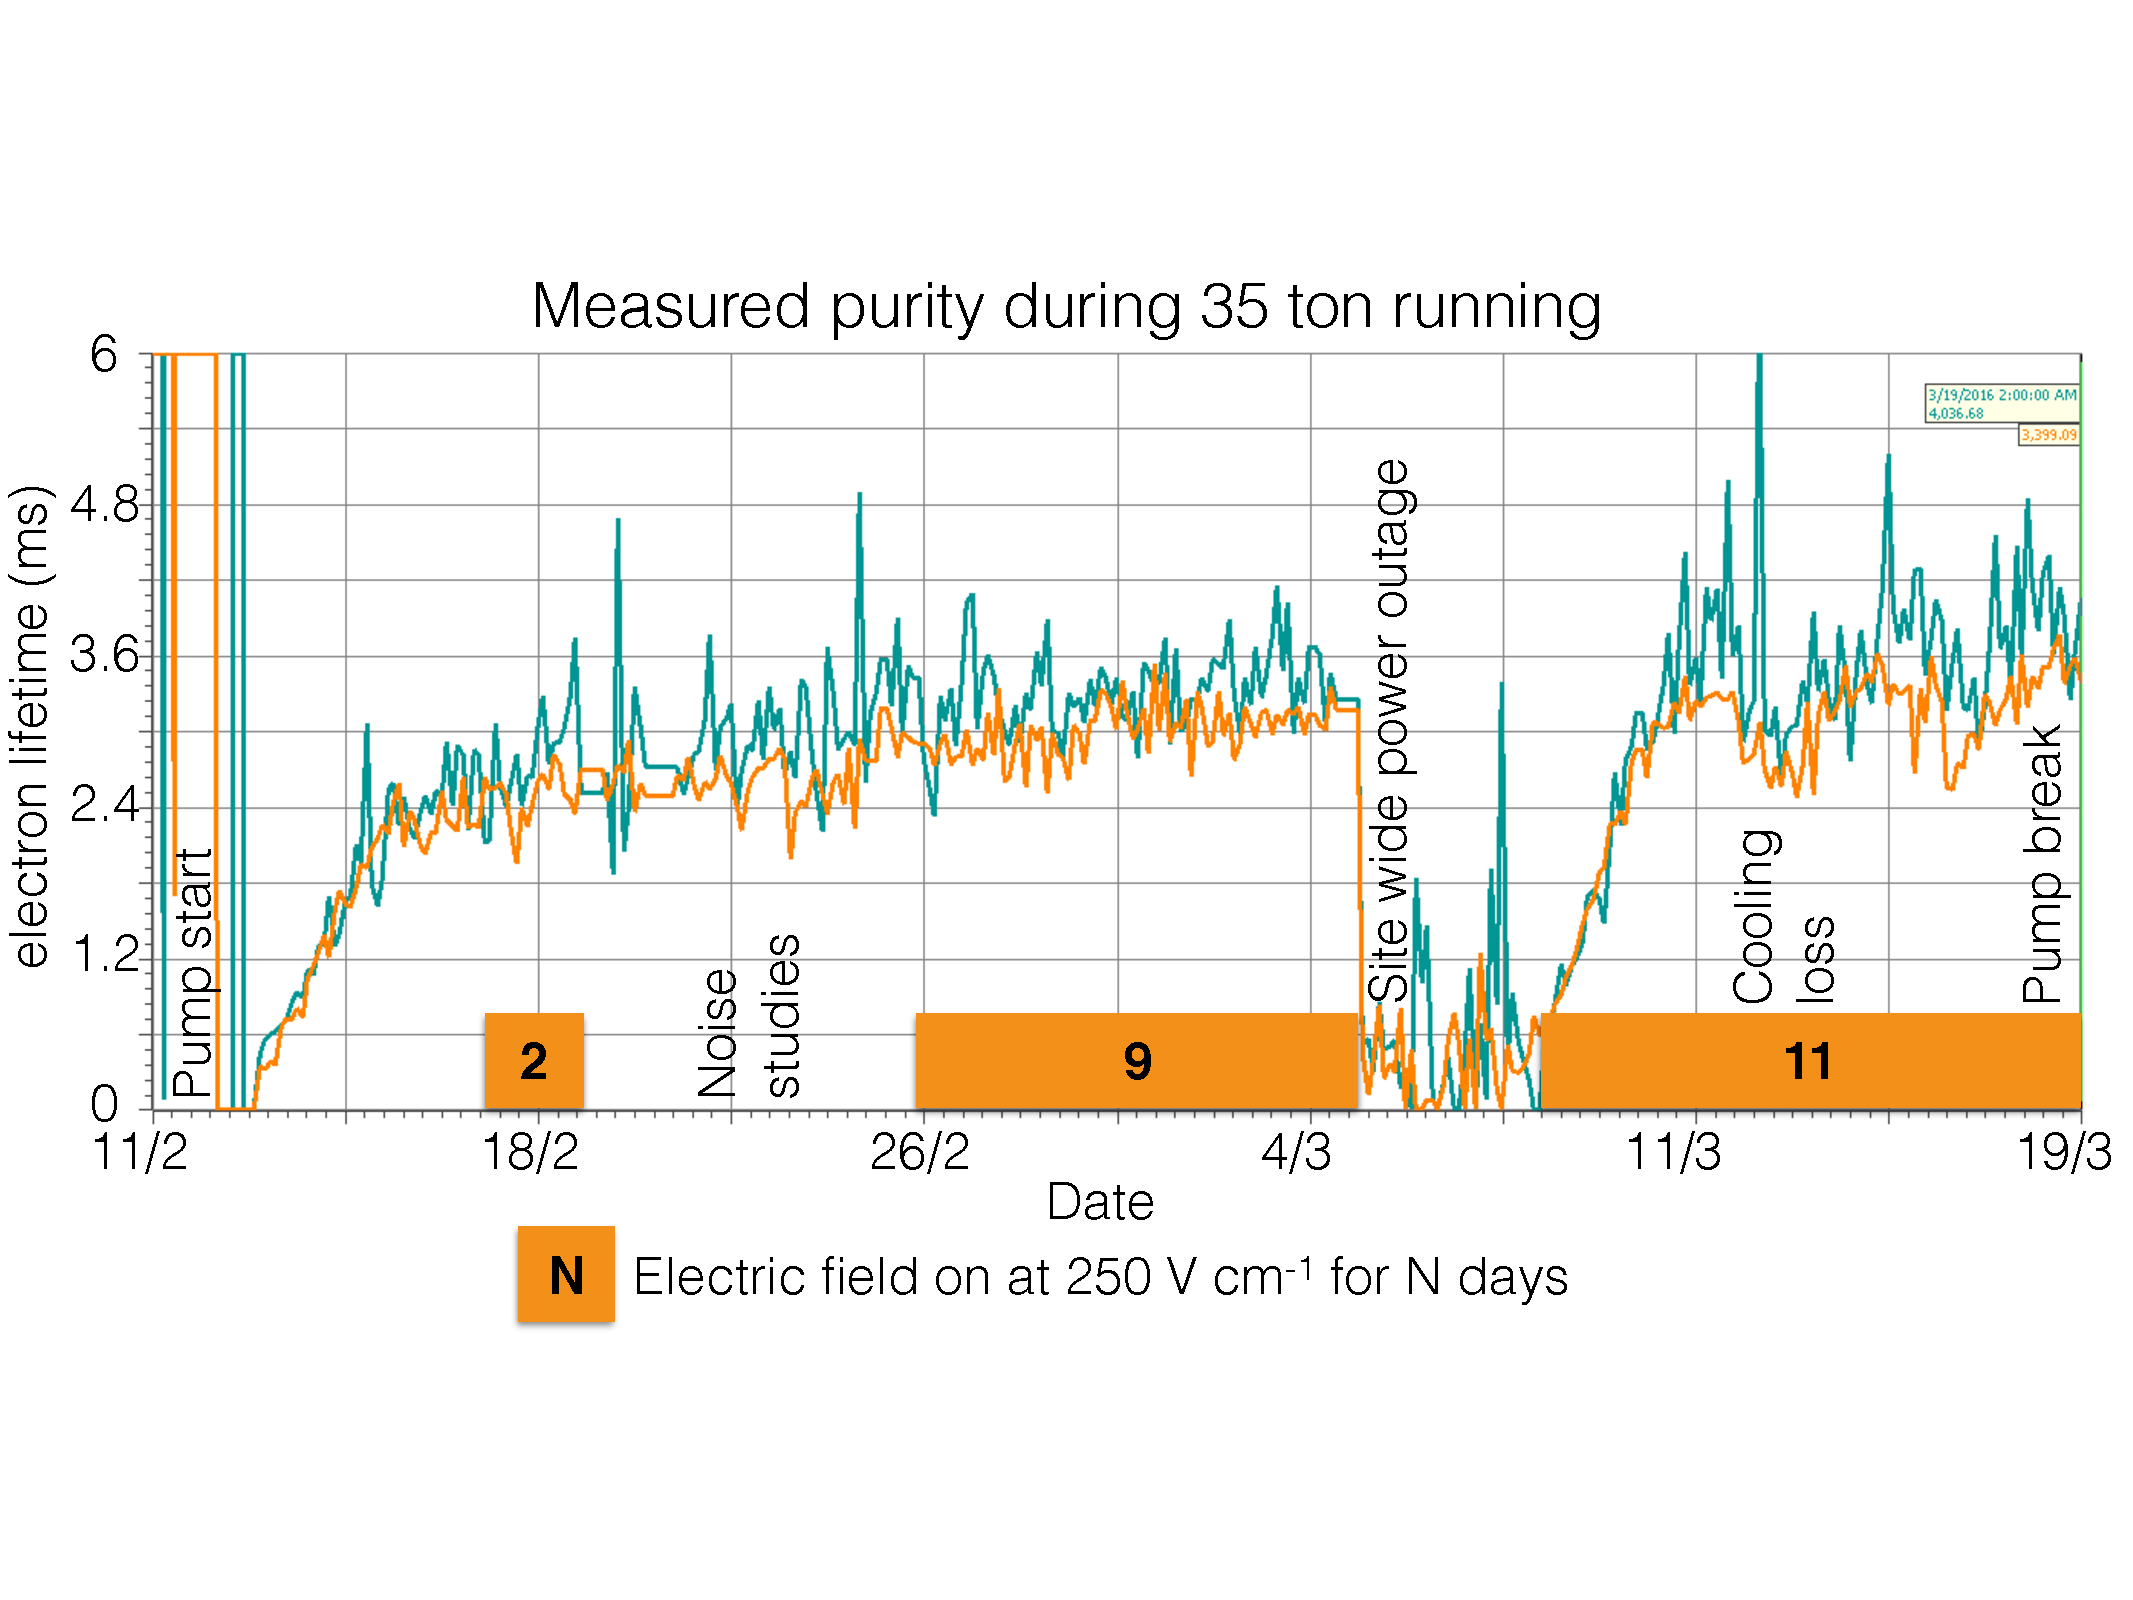
\includegraphics[width=1.0\textwidth]{DataCollected}
  \caption[The 35 ton data sample]{Timeline showing the data collected during the 35 ton Phase II run once the purification pumps were turned on.}
  \label{fig:DataCollected}  
\end{figure}

%********************************** %First Section  **************************************
\section{Organisation of the data structure} \label{Organisation of the data structure} %Section - X.1
As previously noted the 35 ton consisted of three detector sub-systems: RCEs collecting TPC data, SSPs collecting photon detector data, and CRCs tagging cosmic rays. The DAQ combined these three data streams into synchronous events in time saved as LArSoft data objects. These data objects would later have to converted to the offline data products which the reconstruction tools developed on simulation used, this is discussed in Section~\ref{Reformatting the data to the offline structure}. This section describes the structure of the data objects in the raw form.\\

During operations the DAQ was configured to maximise data throughput and physics potential. This meant recording different lengths of times for each of the three sub-systems as the data volumes and length of physics information were significantly different. For example due to the emission of prompt light the physics information from the SSPs is of a much shorter length of time than from the RCEs where data has to be recorded whilst the electrons drift through the LAr. During the running period the recorded data was triggered by through-going muons which produced co-incidences on the CRCs on opposites side of the cryostat. The system used to collect the CRC data was also responsible for generating the triggers and so this meant that the production of triggers could be suppressed to approximately 1 Hz by only producing triggers on the N$^{th}$ co-incidence. A trigger rate of 1 Hz was used as the maximum speed at which data could be written to disk was approximately 60 MB s$^{-1}$, which is roughly equal to the size of each triggered event when the entire detector is read-out in the configuration discussed below. The rate at which events were recorded could have been increased if zero-suppression of the TPC data had been used, however the noise level meant that this was not feasible. \\ 

With an electric field of 250 V cm$^{-1}$ and a drift of 2.25 m, the drift time for electrons at the long drift CPA was roughly 2.6 ms or 5200 ticks (where 1 tick is 500 ns). It was decided that in order for a track causing a counter co-incidence to be separated from other tracks it was necessary to have roughly one drift window both before and after the drift window around the co-incidence, meaning that data was recorded for 7.5 ms or 15,000 ticks around each co-incidence. Only the prompt light from through-going particles was collected and so only 200 $\mu$s of SSP data was recorded for each event. The CRCs produced the least volume of data and so were able to be read out constantly, though the co-incidence triggers were only produced when a trigger was issued. \\

The time synchronous events produced by the DAQ did not however correspond to the physics events, this is because the DAQ was originally designed to produce a continuous data stream. This meant that the DAQ was configured to pad events with headers when a sub-system provided no physics information. Removing these padded header objects was a remit of the online to offline converter discussed in Section~\ref{Reformatting the data to the offline structure}. The length of the DAQ events was configurable and was chosen to be 10 ms (20,000 ticks) in order to best attempt to fully contain physics events and reduce the need for the online to offline converter to stitch DAQ events together. The padding of DAQ events with headers between physics events introduced some peculiarities in the data recorded such as DAQ events containing two parts of non-continuous data as shown in Figure~\ref{fig:DataStructure} where the second DAQ event has no information for the time between the end of physics event 2 and the start of physics event 3.\\

\begin{figure}[h!]
  \centering
  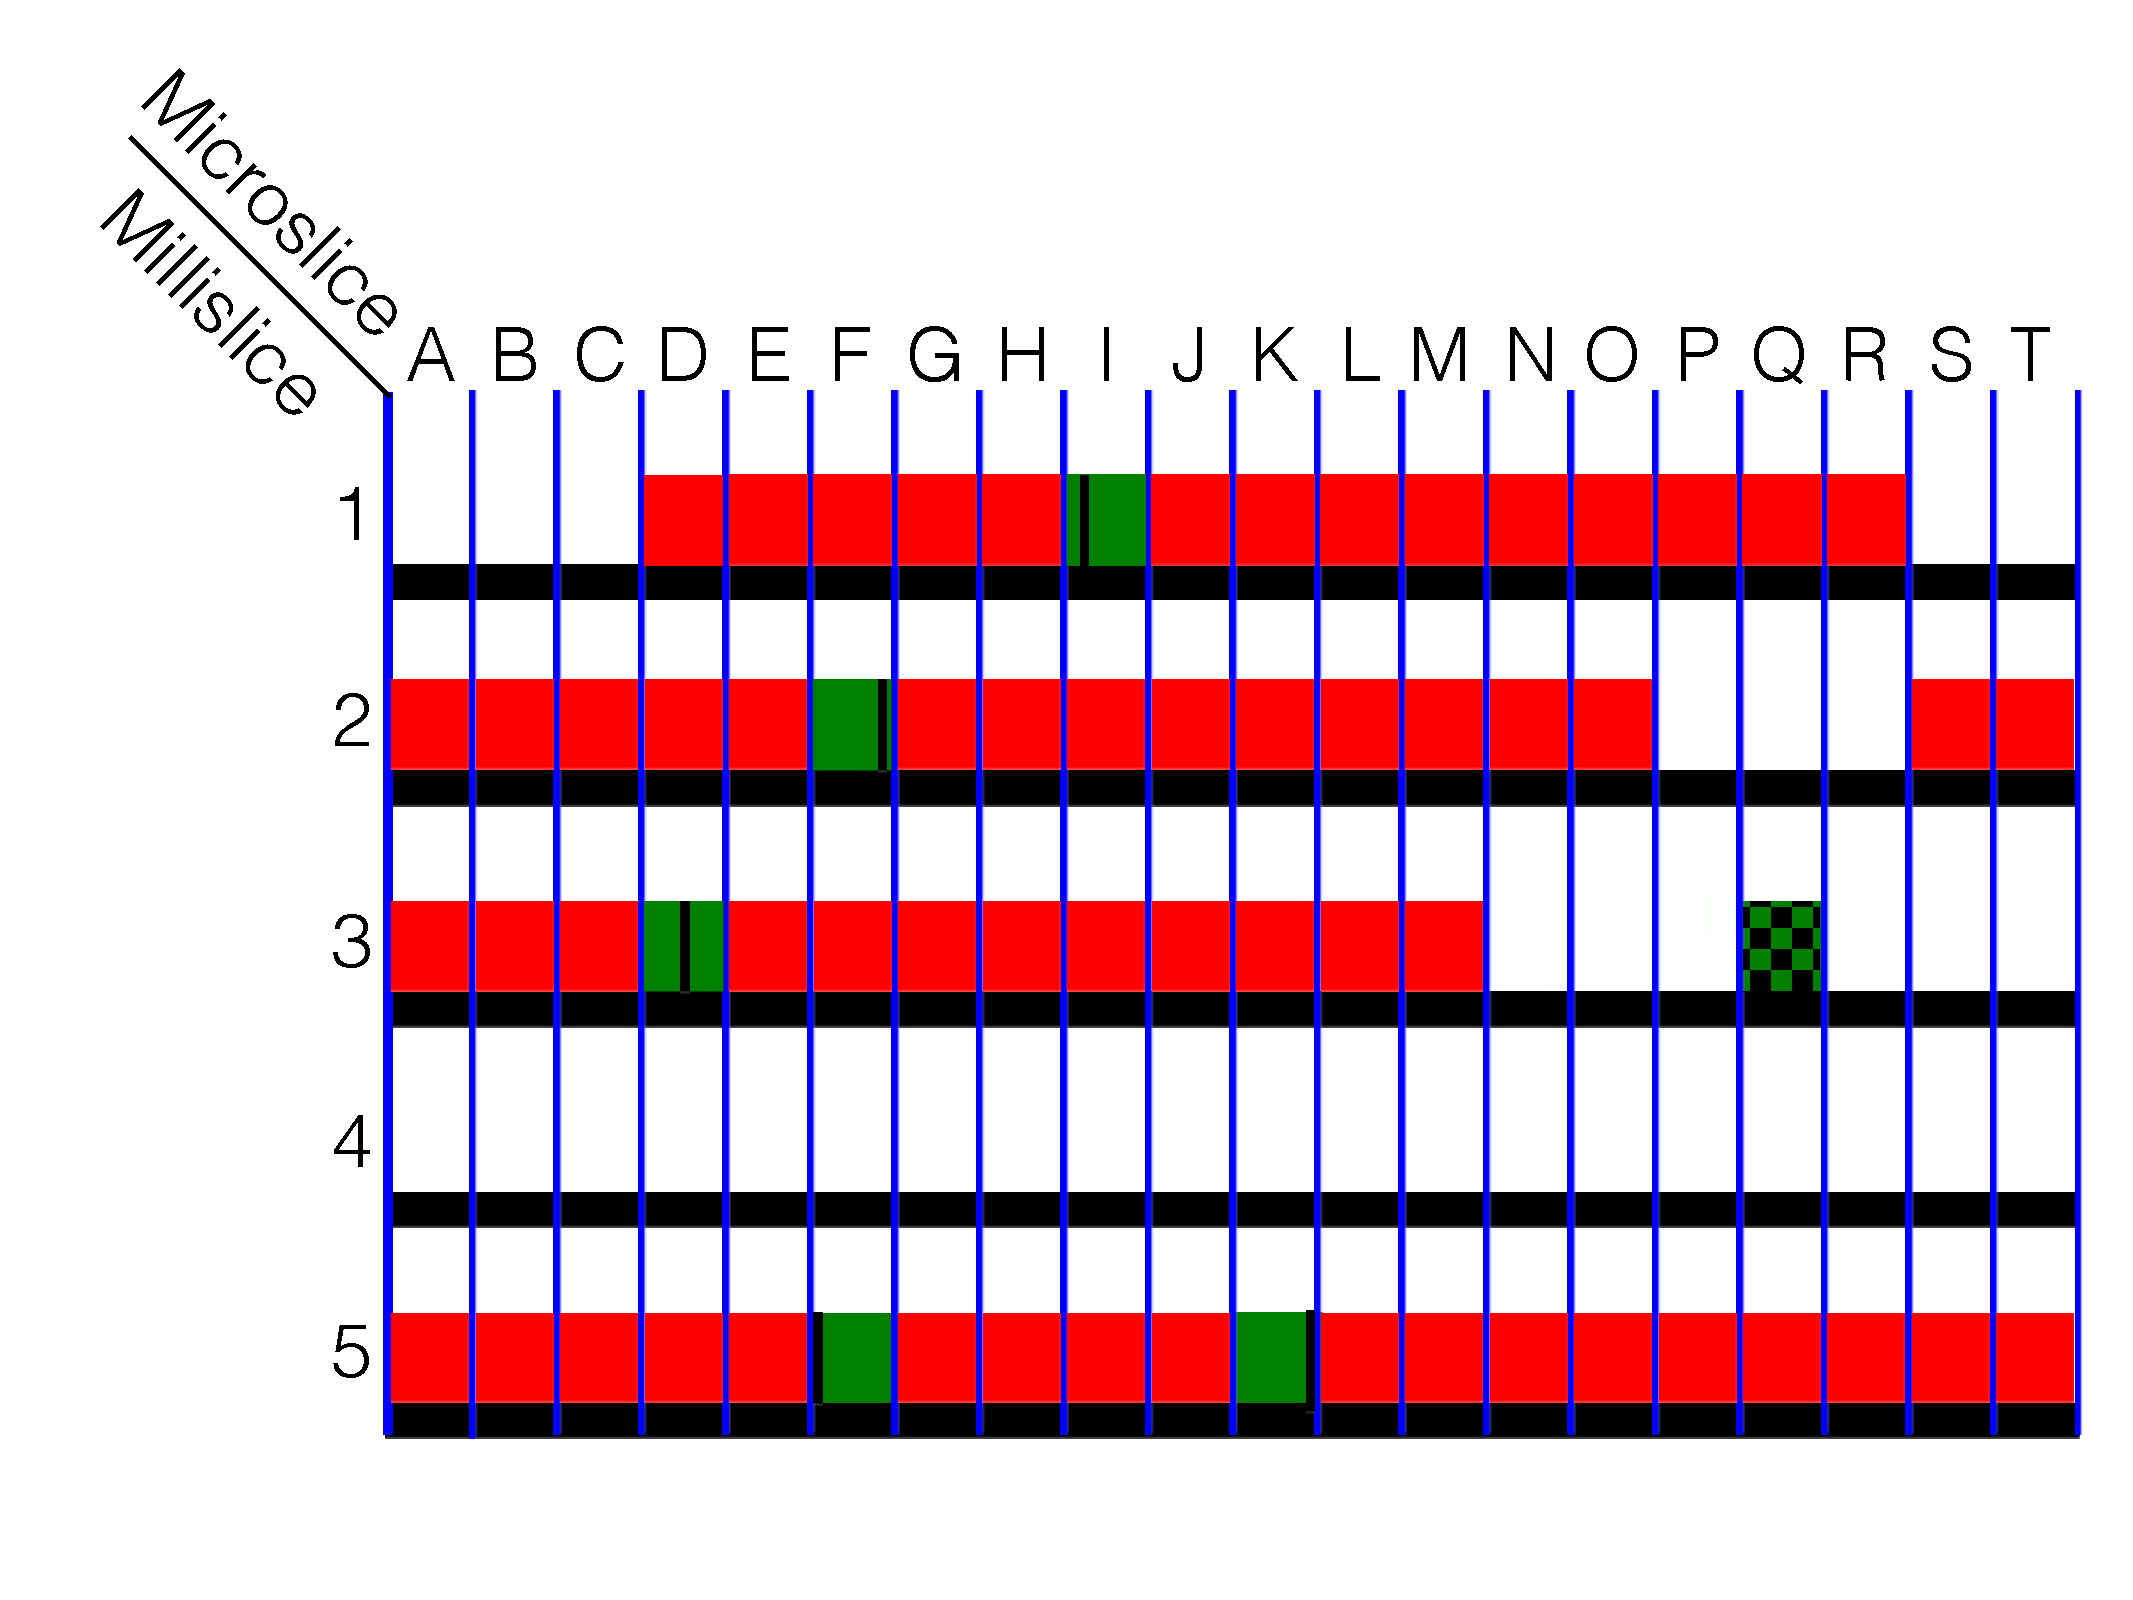
\includegraphics[width=0.75\textwidth]{DataStructure}
  \caption[The 35 ton data structure]{A diagram of possible microslice structures for the TPC data recorded by the 35 ton. Each row represents a single DAQ event, also called a microslice. The vertical blue lines delineate each microslice (0.5 ms, 1,000 ticks). Solid red boxes represent micro slices with TPC data in them, with a group of red boxes being labelled ``physics events''. Green boxes represent triggers which were used with the black lines showing the time in the millislice at which the trigger occurred, and green and black patterned boxes represent triggers which were ignored.}
  \label{fig:DataStructure}
\end{figure}

As the run mode required accessing buffered data it had to be discretised inside the components before being sent to the event builders in the DAQ. In the discussion of how this worked focus will be given on the RCE data where some new terms need to be introduced. Data is collected for every tick on each RCE, where each RCE controls 128 channels. This is called a nanoslice. A microslice is then made by combining N nanoslices such that it contains 0.5 ms (1,000 ticks) of data across all channels. Microslices are then combined to make millislices, where a millislice is synonymous with the DAQ events discussed earlier meaning that 20 microslices are combined to make a millislice. A lack of recorded data means that microslices consist of headers in the place of nanoslices with physics information. \\

During normal data taking the last N microslices are buffered in the RCEs so that if a trigger is issued the previous millislices can be accessed before they are deleted. As the data is buffered in the form of microslices previous microslices may only be accessed in whole. This means that a whole number of microslices must be loaded before the trigger so when a trigger is issued part way through a microslice the previous X microslices are sent to the event builders. As a result during running there are always a minimum number of ticks both before (5,000 ticks) and after the trigger (9,000 ticks) but the exact numbers can change by up to 1,000 ticks for a given event depending on where in a microslice the trigger came. This is shown in Figure~\ref{fig:DataStructure} where the black lines representing triggers are seen to occur at different points within the microslices, for example physics event 1 will have more data after the trigger than physics event 2 as the trigger occurs earlier in the triggered microslice.

%********************************** %Second Section  *************************************
\section{Reformatting the data to the offline structure} \label{Reformatting the data to the offline structure} %Section - X.2
Conversion of the data objects stored in the raw data to the data objects used in simulation required a suite of unpacking services to be written, the specifics of which are not discussed here. These all required a common interface through which to access the data and check that the timing of each component was consistent and then to produce a final LArSoft file for downstream use. This interface had the added role of producing complete physics events, meaning that it had to be able to combine multiple millislices and extract only the data containing the continuous physics events. \\

The format that the data reformatter followed was that following the unpacking of each of the sub-systems the TPC ticks would be looped through to see if a user defined set of conditions could be satisfied. These conditions were usually whether an East-West or North-South counter co-incidence occurred at that time, or if the current millislice contained TPC data whilst the previous one did not. The latter was the default configuration as this gave the option of preserving all of the data gathered, for reasons discussed at the end of Section~\ref{Organisation of the data structure}. Other conditions were available though rarely used such as if the SSPs observed a large flash of flight or if there was a large change in the average TPC ADC value. Once a set of conditions is satisfied a user defined number of pre-condition ticks are gathered, clearly this is set to zero in the case of the previous millislice containing no TPC data as there is no previous data to load which would not have a gap in time, see Figure~\ref{fig:DataStructure}. In the case of using a counter co-incidence to make an event a value of 300 pre-condition ticks is normally used. Once the pre-conditions ticks are gathered a further N post-condition ticks are gathered, where N is defined by the user. Usually 15,000 ticks are gathered when the previous millislice is empty and 5,200 ticks are gathered when there is a co-incidence. Data from the other components is added to the event if its timestamp is within the timestamps of the first and last ticks in the event when no more TPC data is required or at the end of a millislice if stitching is required. All timestamps are corrected such that the event began at T=0 as the reconstruction assumes this and the timestamp of the start of the event is stored in the event record so that it can be accessed downstream if required. \\

At all points in this process it is important to integrate flexibility so that the user can choose the length of events, which sub-systems are in the events and what the conditions are for making events. It was also important for users to be able to run the service on already formatted events as the unpacking services were the major overhead in running the interface. It is also conceivable that users would want to reformat Monte Carlo events so as to centre them around their chosen conditions and so the use of the unpacking was determined by the interface depending on the format of the input file.

%********************************** % Third Section  *************************************
\section{Observations on data quality and noise mitigation} \label{All the noise} %Section - X.3
Reformatting the online data to the offline format was an important step in maintaining data quality as subsequently there was no access to the raw data due to how the DUNE software is established. Some of the important checks which were performed are outlined in Figure~\ref{fig:DataDrops}. If any of these issues were present in a given physics event then it is discarded as the integrity of the data cannot be guaranteed. It was decided that these events would be discarded as non-synchronous events would lead to hits in the detector being at incorrect times and padding empty events with pedestals could mean that tracks seem to disappear and later reappear as they travel through the detector. \\

Another example of inconsistent events is when the sub-systems are not synchronised with each other, this is normally caused by one of the sub-systems missing a clock increment from the master timing unit due to the data trigger being issued close to an increment from the master unit. This misalignment causes an incorrect time sample being read out and so the data from each sub-system within a millislice is not consistent meaning that it will fail the timestamp check and so won't be added to the event record. To avoid incomplete events these physics events are also discarded when observed. \\

\begin{figure}[h!]
  \centering
  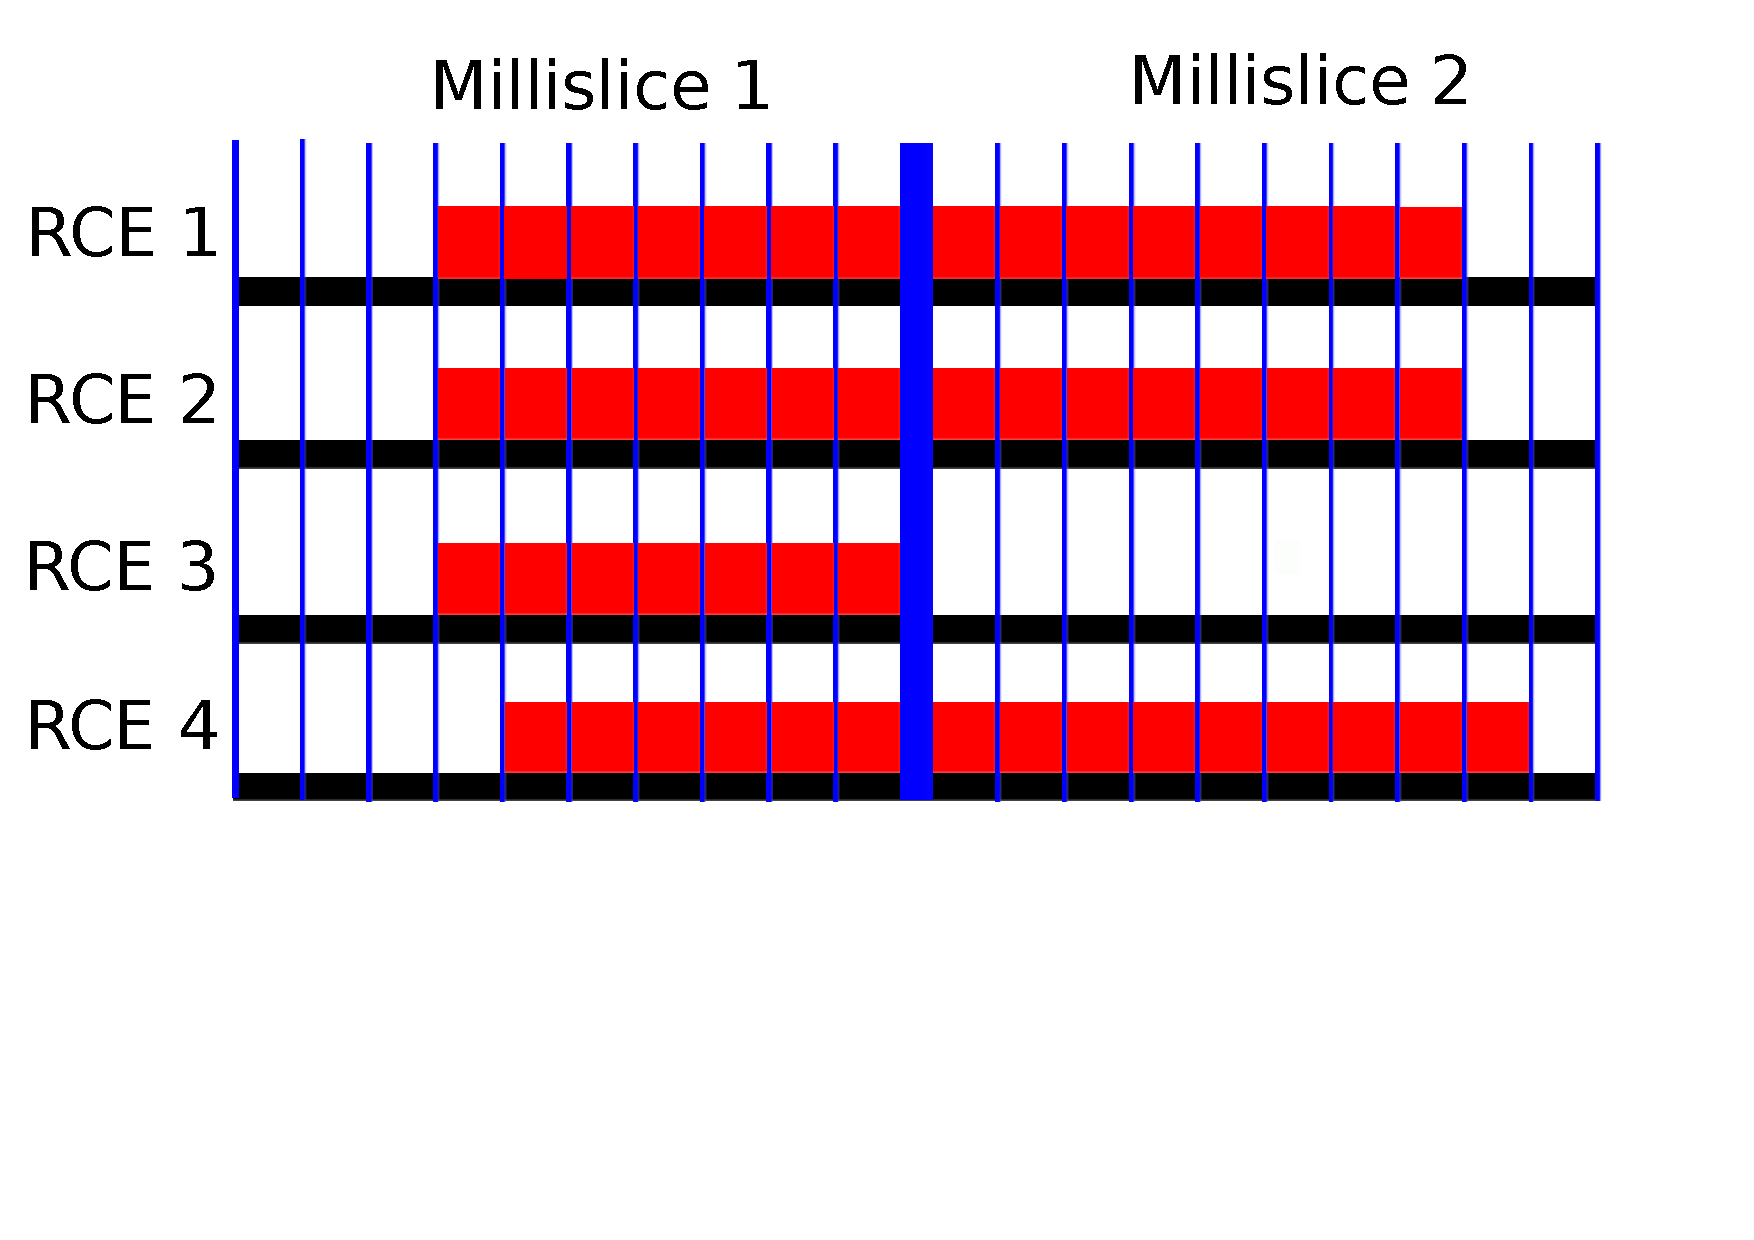
\includegraphics[width=0.85\textwidth]{DataDrops}
  \caption[Dropped TPC data in the 35 ton]{A diagram of how TPC microslices can be saved in millislices in the 35 ton. Two millislices are shown, each containing 10 microslices. One physics event straddling the millislice boundaries is shown and 4 RCEs representing each row are read out. The vertical blue lines delineate each microslice (0.5 ms, 1,000 ticks), with the thick blue line showing the millislice boundary. Solid red boxes represent micro slices with TPC data in them. It can be seen that RCEs 1 and 2 contain data for the same interval, whilst the data from RCE 3 in millislice 2 has been ``Dropped,'' and the data from RCE 4 is shifted by 1 microslice from RCEs 1 and 2 and is thus ``Inconsistent.'' As a result of these issues this physics event would be discarded as data integrity cannot be guaranteed.}
  \label{fig:DataDrops}
\end{figure}

The electronic noise in the 35 ton was higher than anticipated, with the RMS of the RCE ADC being approximately 30 counts compared to an expected thermal noise of around 2.5 ADC counts. Many sources contributed to this elevated noise, some of which are explained below. \\

Though not directly affecting the noise issues stuck ADC codes were a feature of the data which had to removed downstream. Stuck ADC codes were caused by the 6 least significant bits getting frozen to either 000000 or 111111, this was observed during the first stages of commissioning and an algorithm to remove them was developed and tested on Monte Carlo. In simulations it was observed that the signal could be recovered with minimal losses, as shown in Figure~\ref{fig:StuckCodes} where the blue lines (after removal) are seen to closely match the black lines (before adding stuck codes). \\

A significant portion of the noise was correlated between groups of 32 channels, where the ADCs would coherently oscillate. To remove these coherent shifts ADC baselines were calculated for these groups of 32 channels at each tick and then subtracted from the measured ADC values. This was found to be an effective method of removing coherent noise in MicroBooNE \citep{uBooNENoise}. The effect of removing coherent noise is shown in Figure~\ref{fig:CoherentNoise}, where the signal peak becomes much easier to discern after noise removal and a coherent noise peak around tick 6030 is removed. An issue with removing coherent noise in this way is that events which are parallel to the APAs will produce signals at common times across adjacent wires and these signals may be removed along with the coherent noise causing a reduction in the hit reconstruction efficiency. The only way to prevent this is to ``protect'' potential signal regions from the coherent noise removal, as is done in MicroBooNE \citep{uBooNENoise}. \\

When a Fast Fourier Transform (FFT) \citep{CoTuFFT} is performed on the coherent noise subtracted waveforms it can be seen that signals occur with specific frequencies. Some of these frequencies are caused by real energy depositions, whilst others are due to the electronics noise. It is possible to remove the noise frequencies by applying Wiener filters \citep{WienerFilter}. Frequency spectrum's are taken for each of the three planes and a clear signal is both preserved and suppressed. The raw signal spectra are then divided by the signal suppressed spectra to produce $signal/noise$ frequency spaces. The signal regions to be conserved can then be found by fitting a combination of sigmoid functions to the frequency spaces around regions of high $signal/noise$. A demonstration of how this applied is shown in Figure~\ref{fig:FrequencyFilter}. It is also possible to remove specific frequencies which are not removed by the filters, this was necessary for a 54 KHz noise component introduced by the fluorescent lights in the detector hall. After the run ended it was found that some of the high frequency noise components were introduced by a short on a warm power cable, the techniques used to find this cable will be used when commissioning future detectors \citep{35tonNoiseMeeting}. \\

\begin{figure}[h!]
  \centering
  \begin{subfigure}{0.45\textwidth}
    \centering
    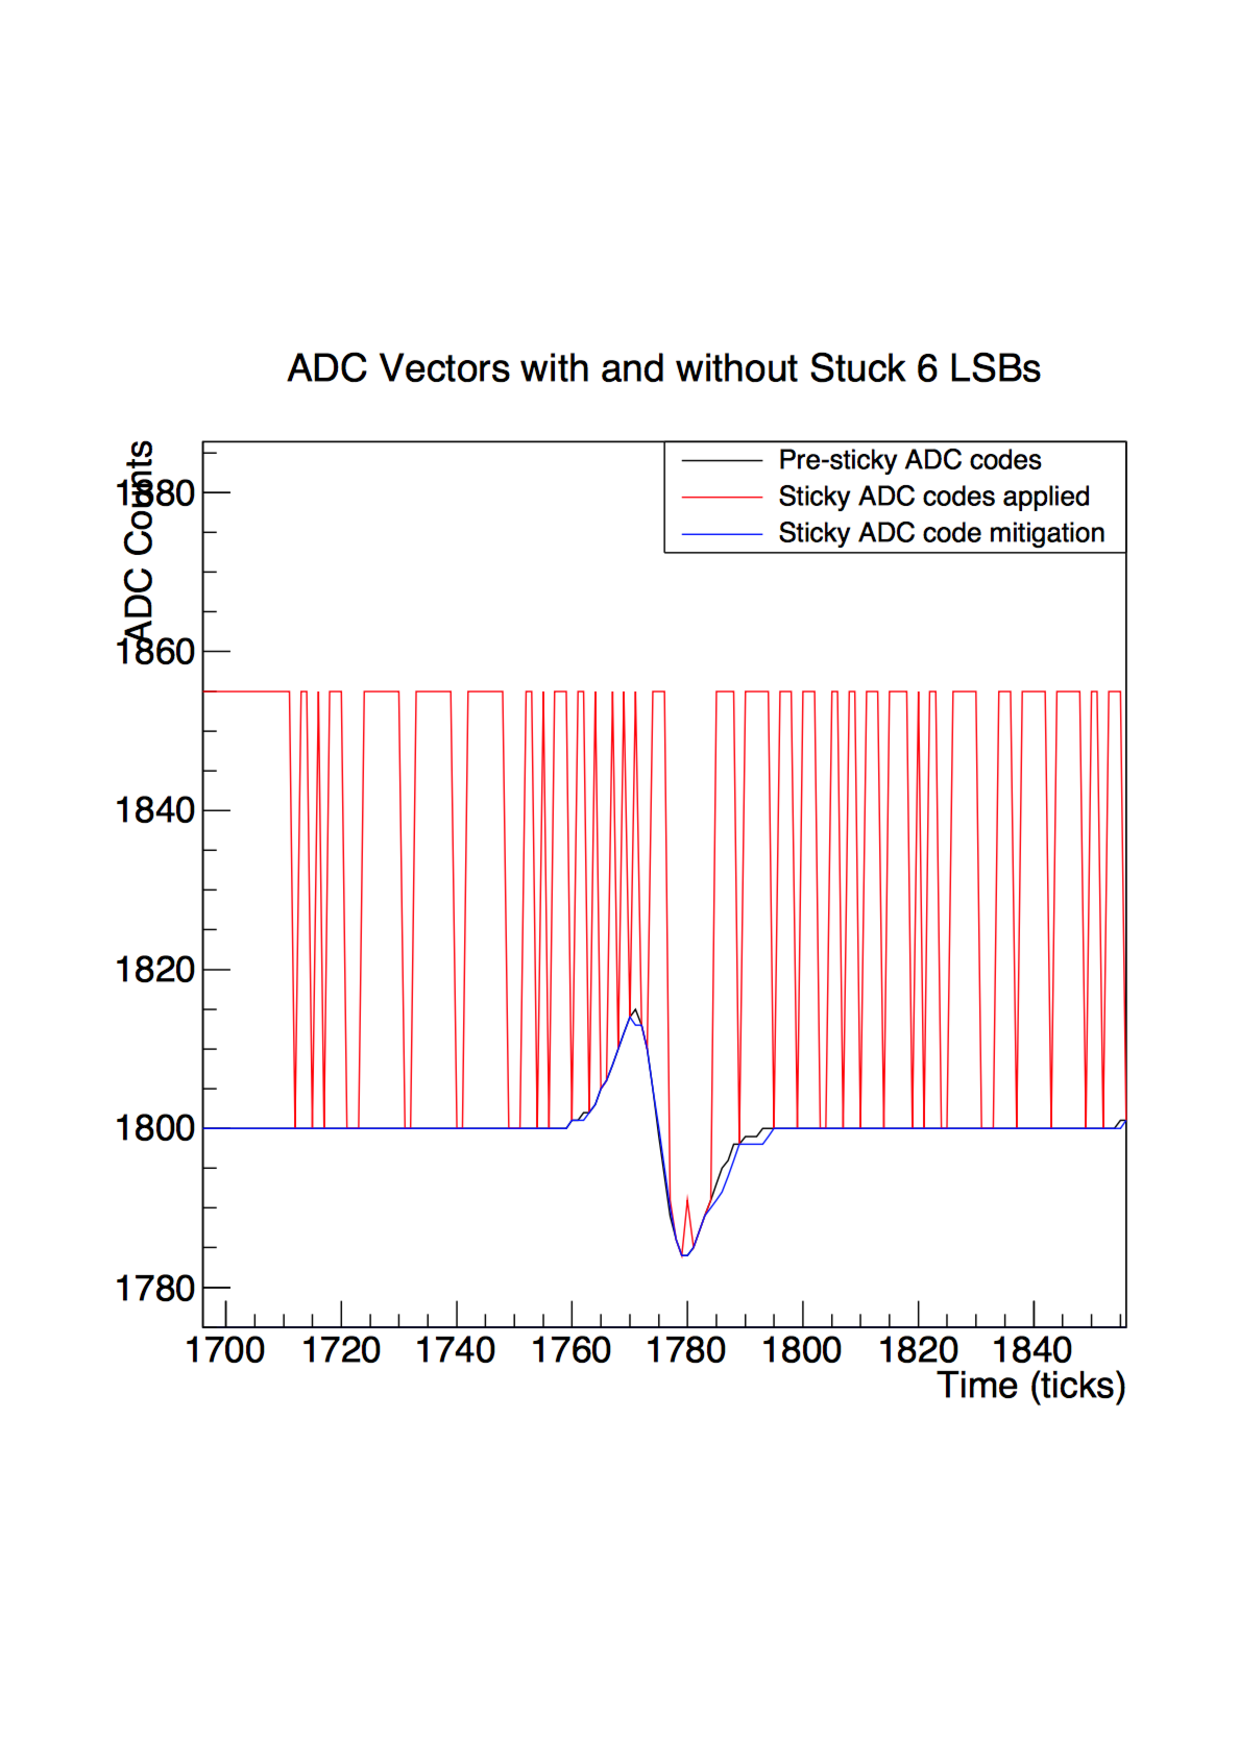
\includegraphics[width=\textwidth]{StuckCodes}
  \end{subfigure}
  \hspace{0.08\textwidth}
  \begin{subfigure}{0.45\textwidth}
    \centering
    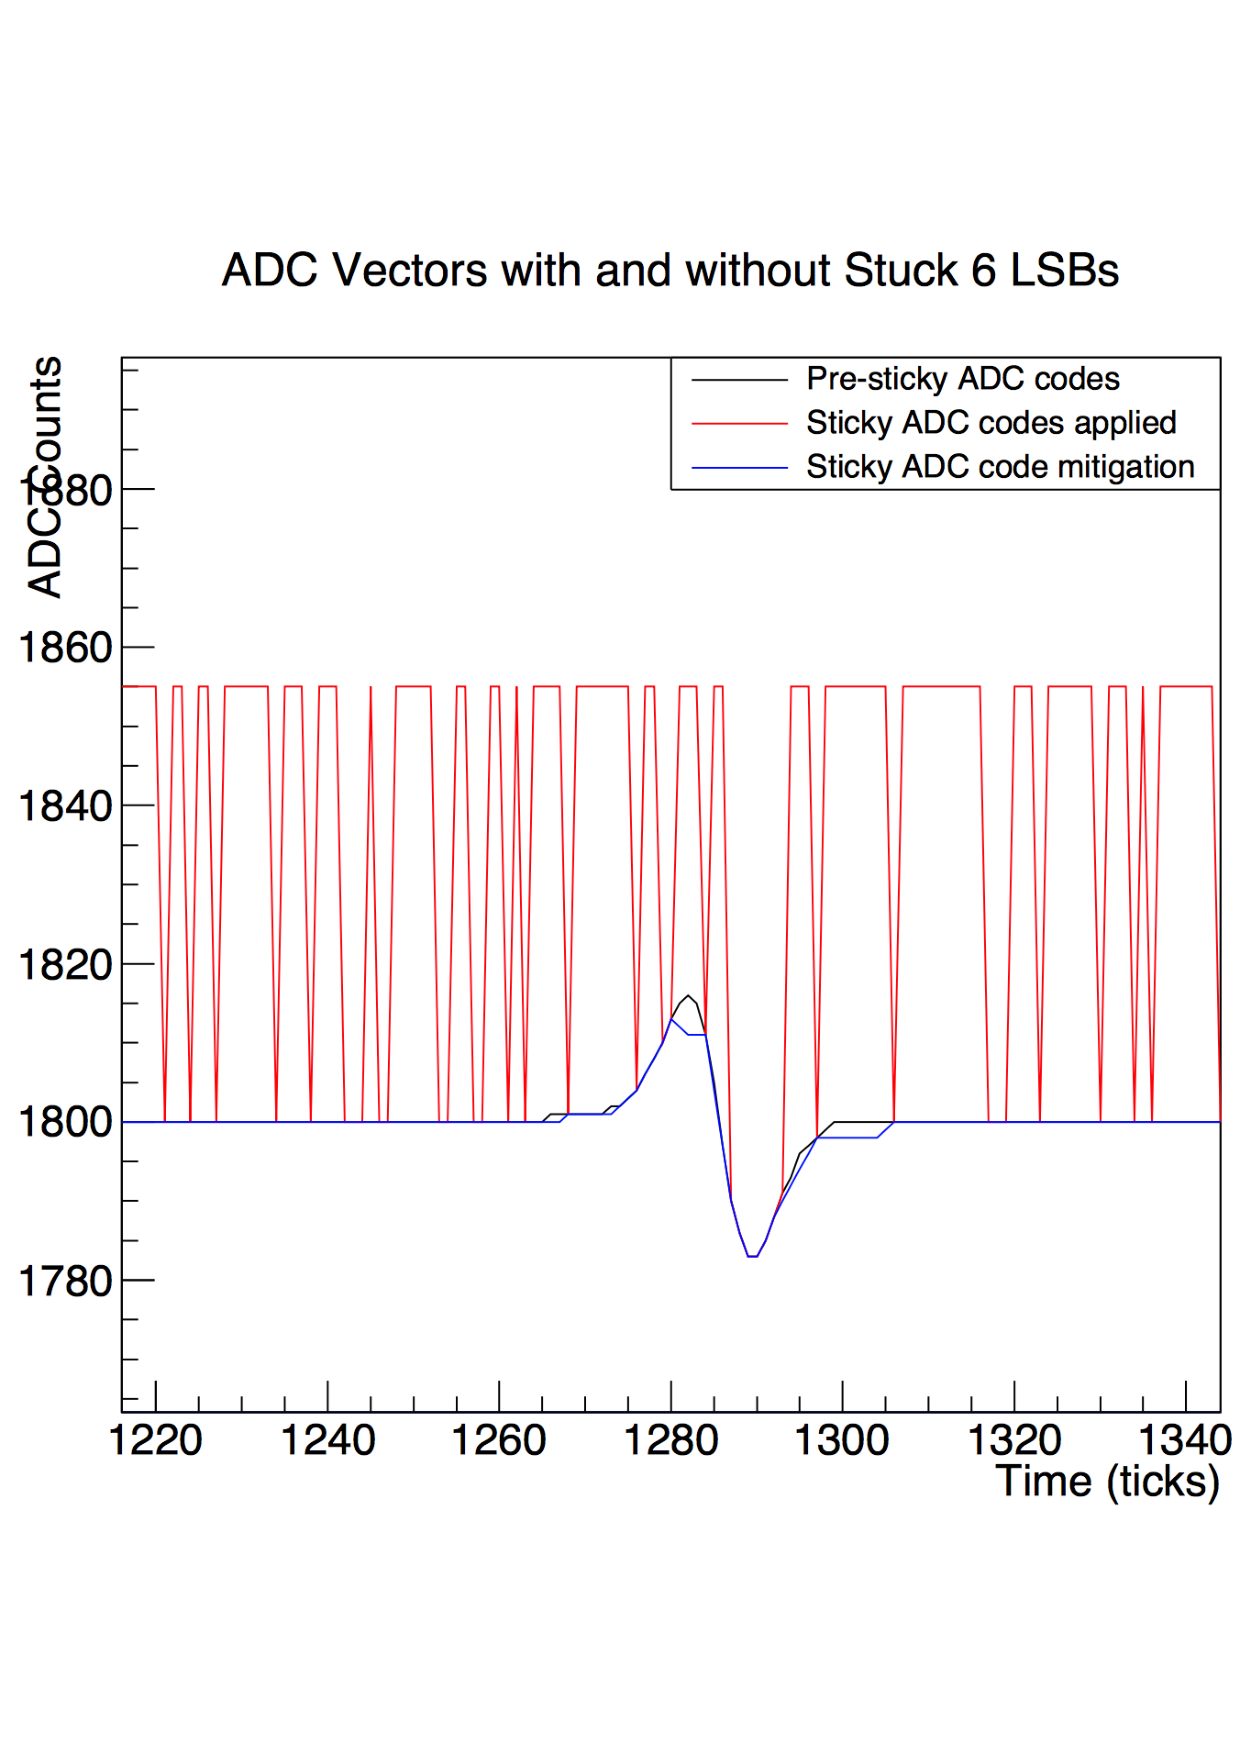
\includegraphics[width=\textwidth]{StuckCodes2}
  \end{subfigure}
  \caption[Recovering stuck ADC codes in the 35 ton]
          {Two Monte Carlo spectrum's showing the effect of the introduction and removal of stuck bits on a simulated signal \citep{InslerStuckCode}.}
          \label{fig:StuckCodes}
\end{figure}

\begin{figure}[h!]
  \centering
  \begin{subfigure}{0.45\textwidth}
    \centering
    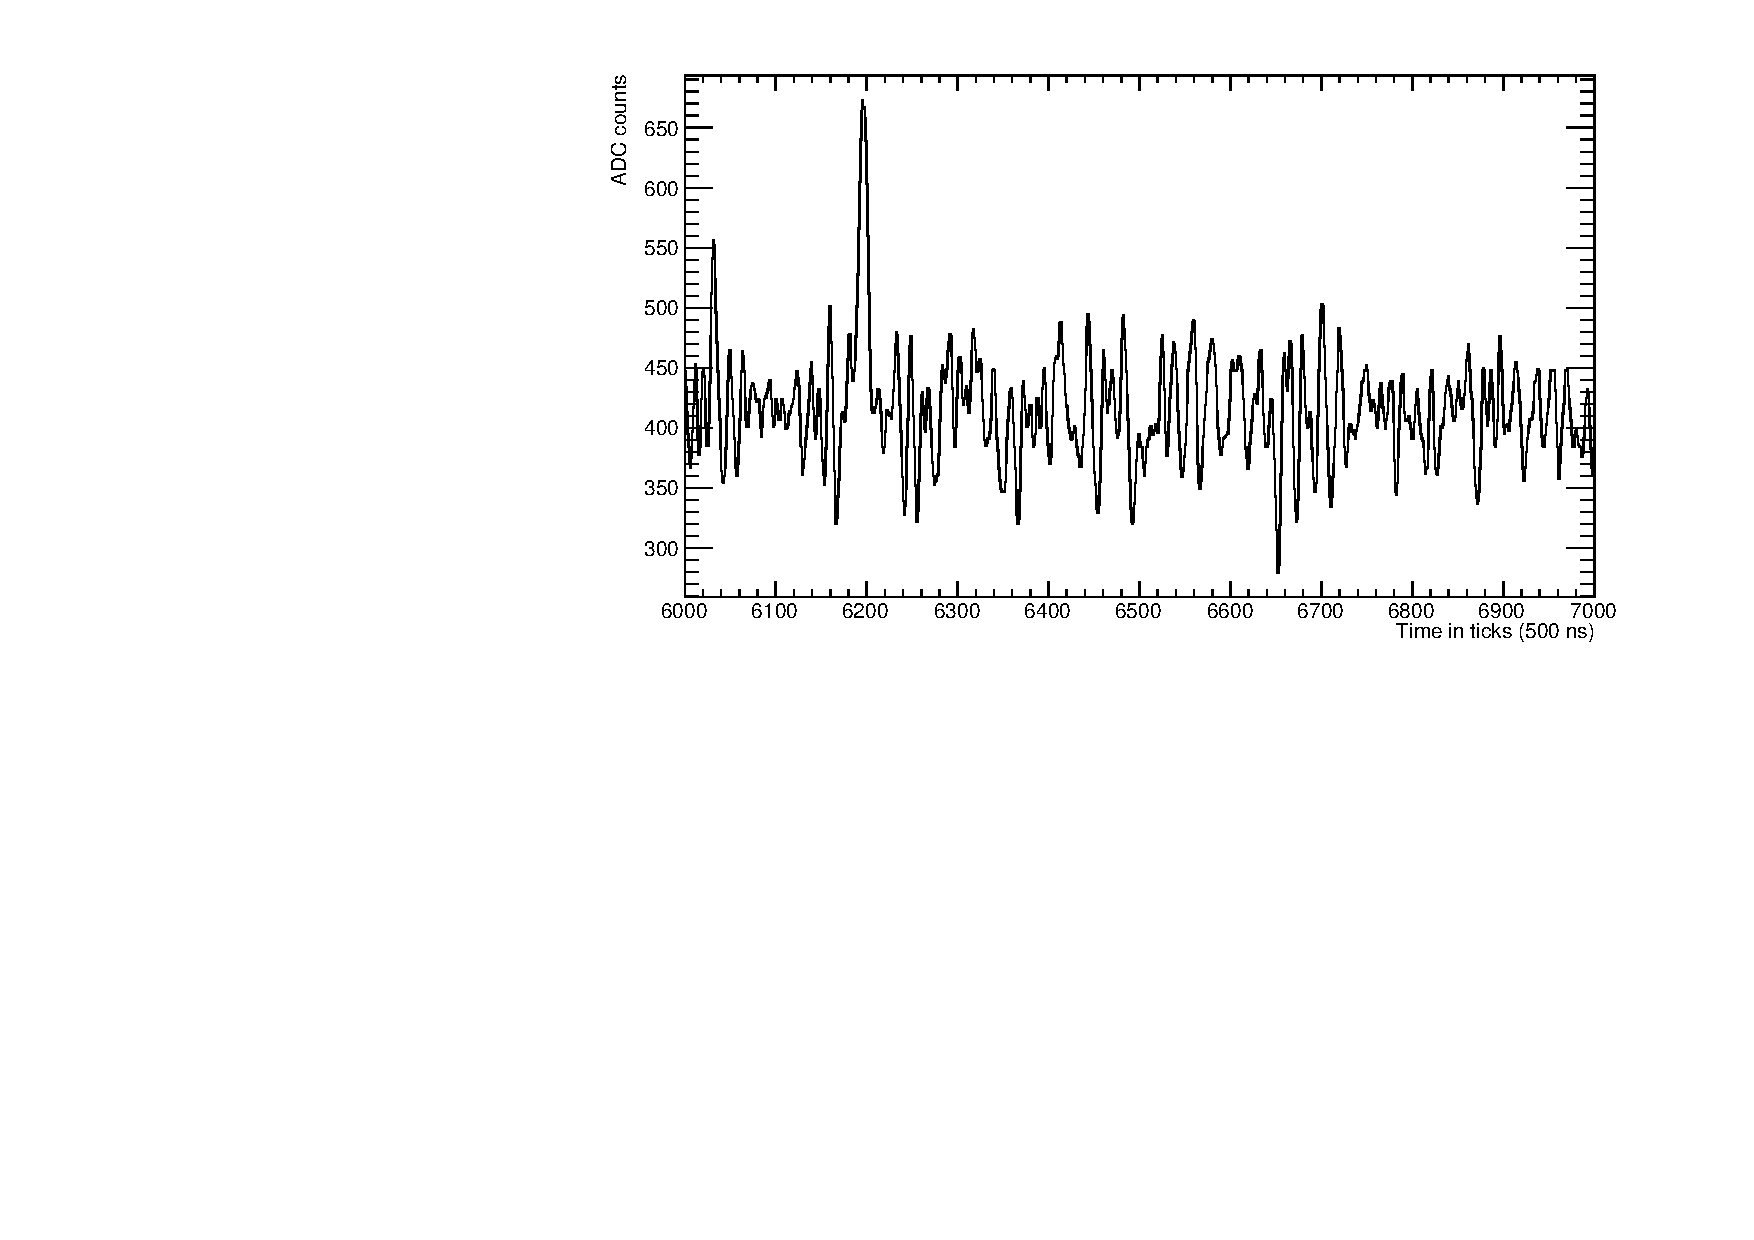
\includegraphics[width=\textwidth]{BeforeCoherent}
    \caption{Before coherent noise removal}
  \end{subfigure}
  \hspace{0.08\textwidth}
  \begin{subfigure}{0.45\textwidth}
    \centering
    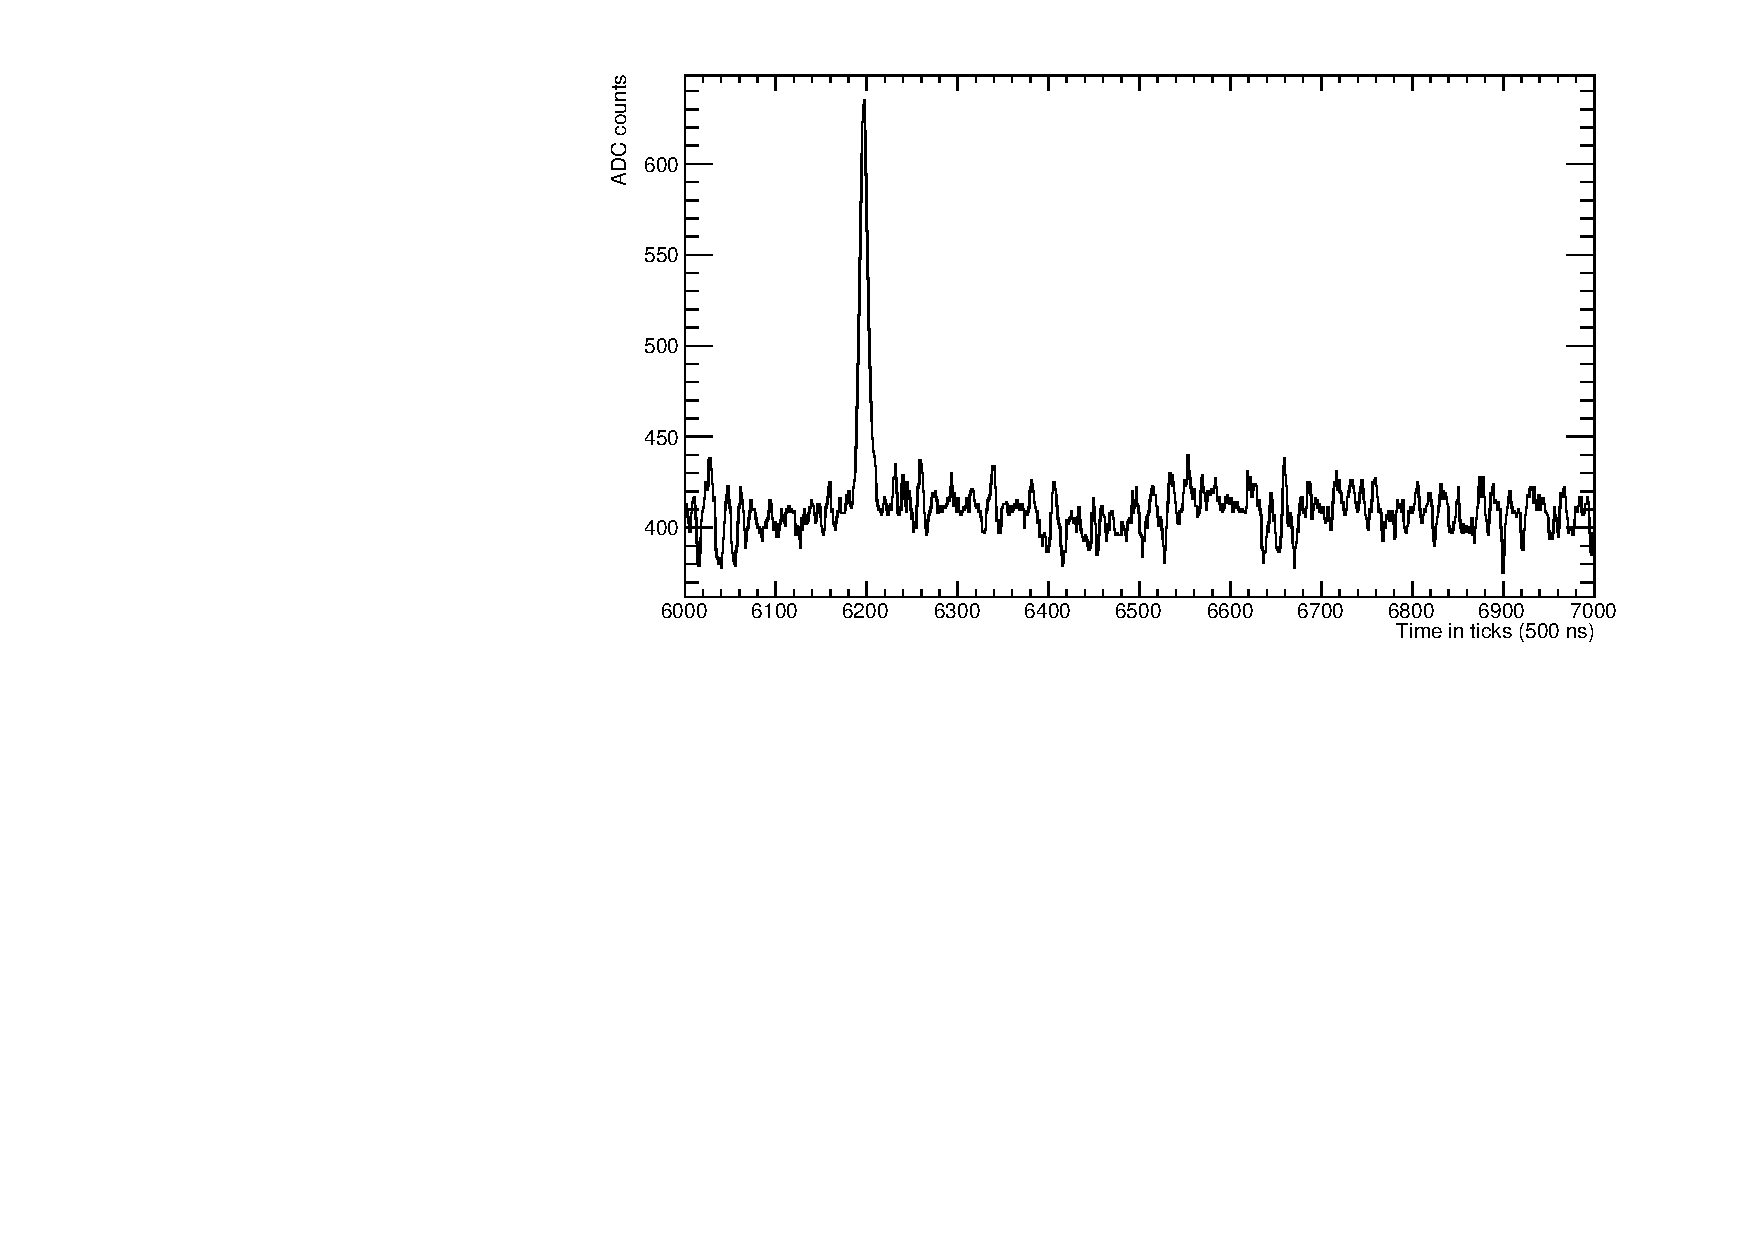
\includegraphics[width=\textwidth]{AfterCoherent}
    \caption{After coherent noise removal}
  \end{subfigure}
  \caption[Removing coherent noise in the 35 ton]{The effect of coherent noise removal on a 35 ton signal event.}
  \label{fig:CoherentNoise}
\end{figure}

\begin{figure}[h!]
  \centering
  \begin{subfigure}{0.45\textwidth}
    \centering
    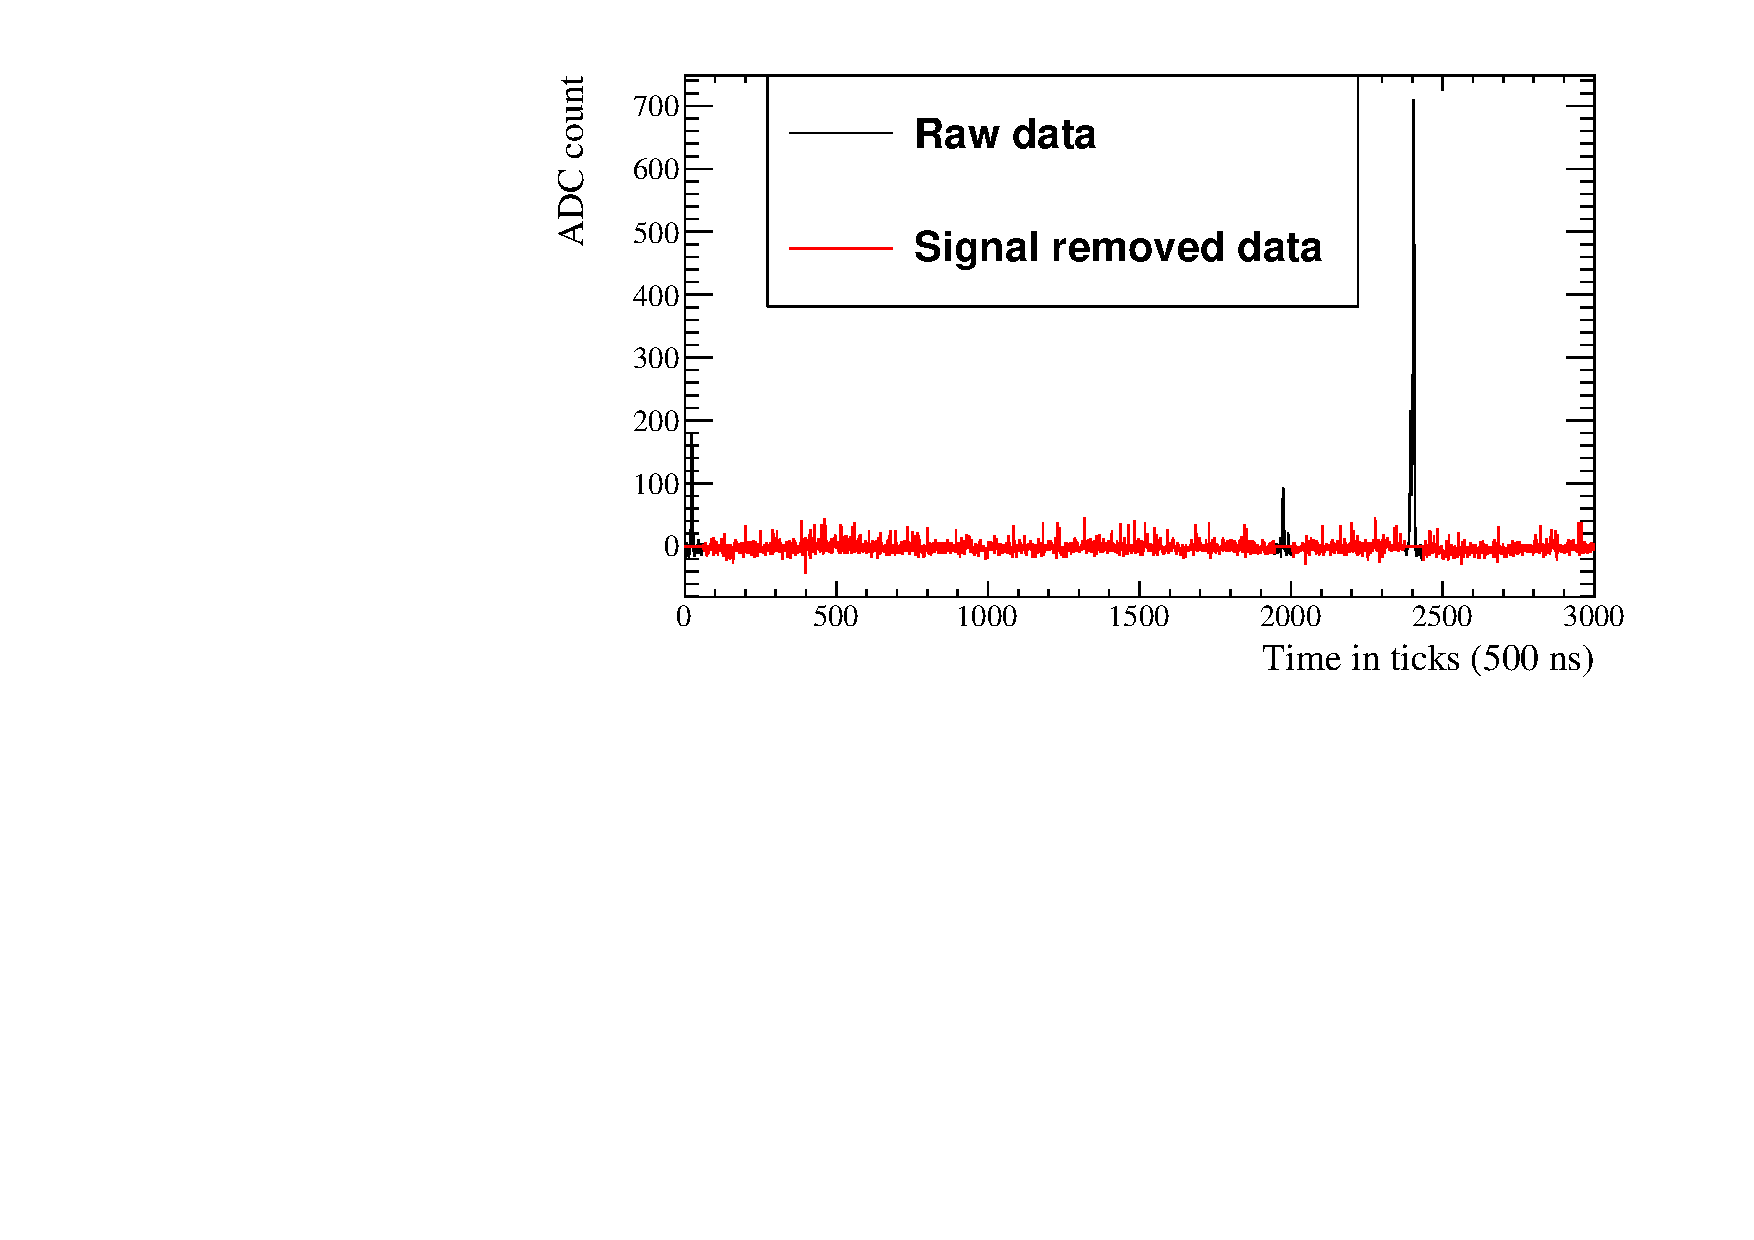
\includegraphics[width=\textwidth]{Waveforms}
    \caption{A raw and signal subtracted waveform for a collection plane wire.}
    \label{fig:FreqWaveform}
  \end{subfigure}
  \hspace{0.08\textwidth}
  \begin{subfigure}{0.45\textwidth}
    \centering
    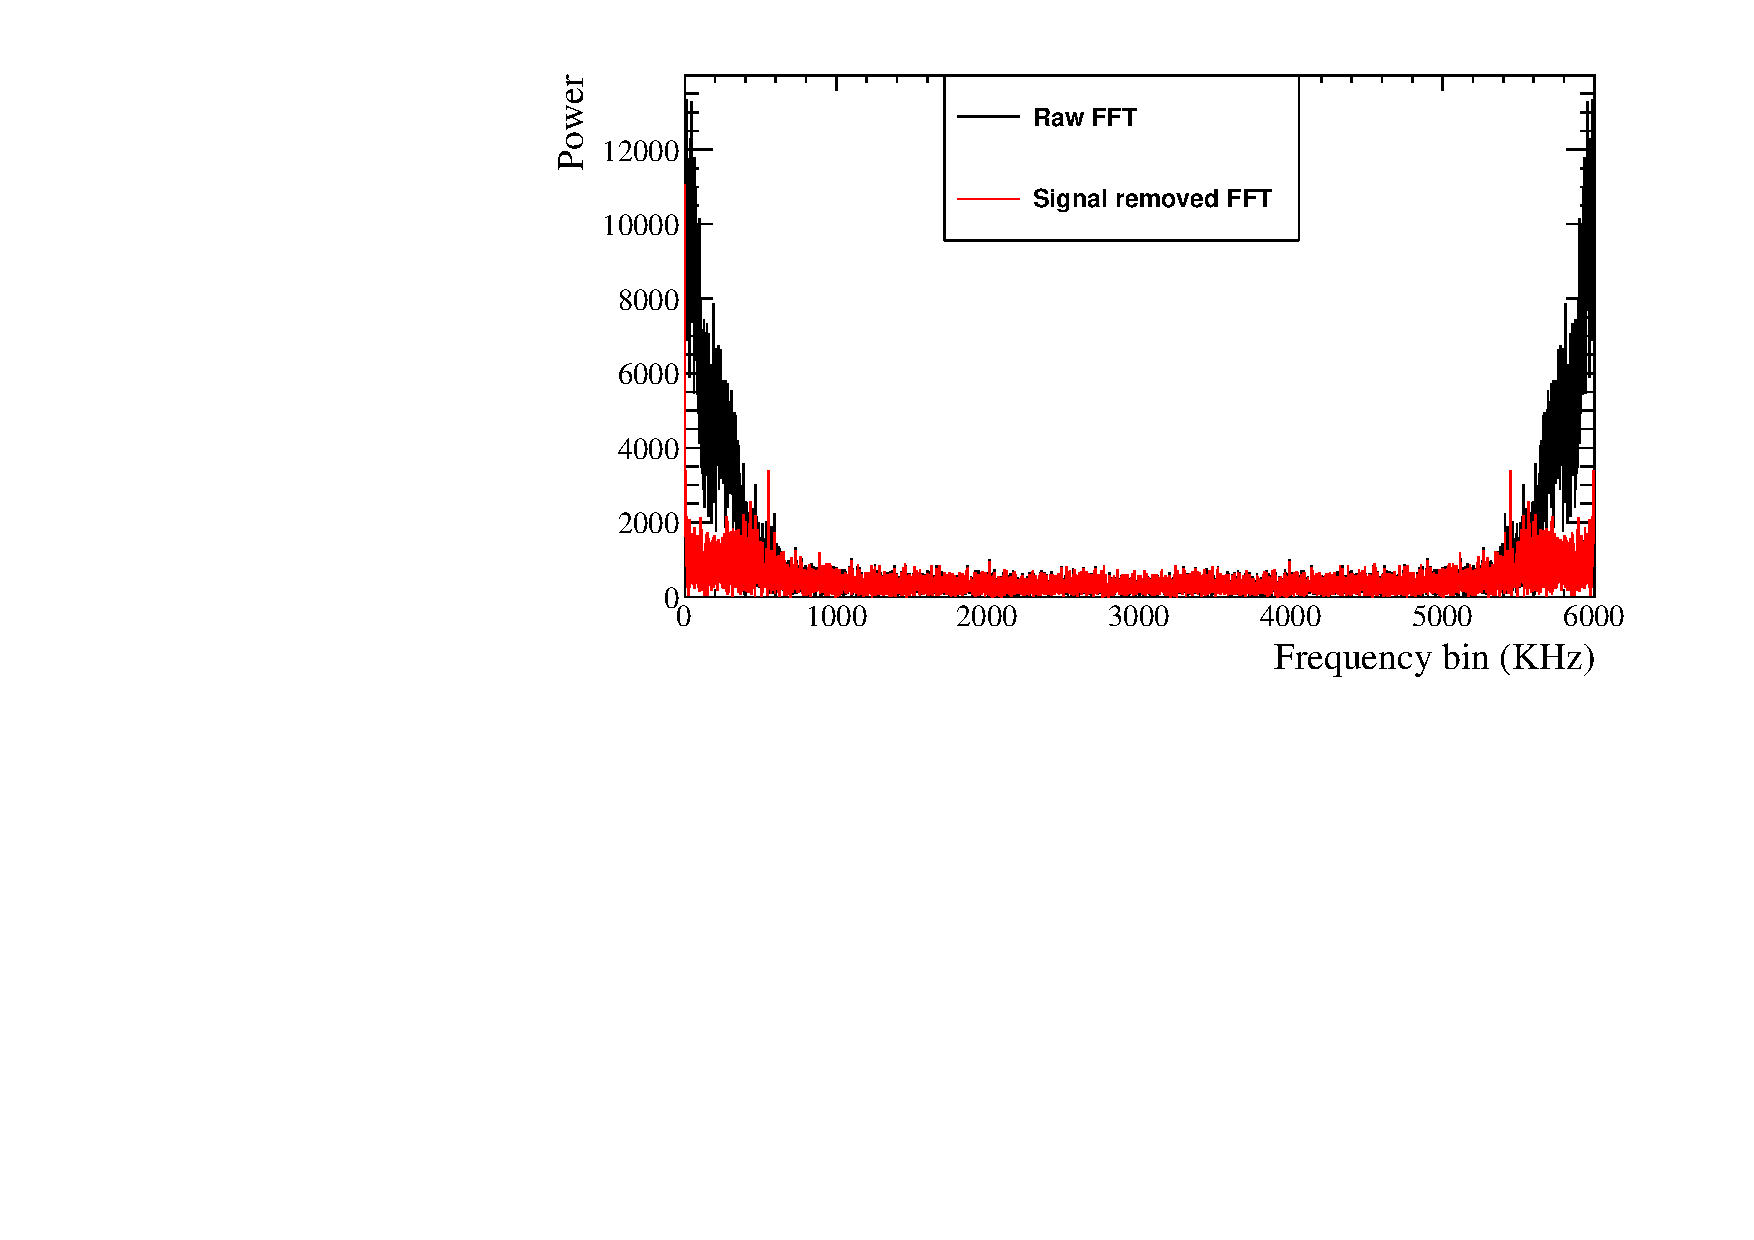
\includegraphics[width=\textwidth]{NoiseFFTs}
    \caption{The FFT of the raw and signal subtracted waveform for a collection plane wire.}
    \label{fig:FreqFFT}
  \end{subfigure}
  \begin{subfigure}{0.45\textwidth}
    \centering
    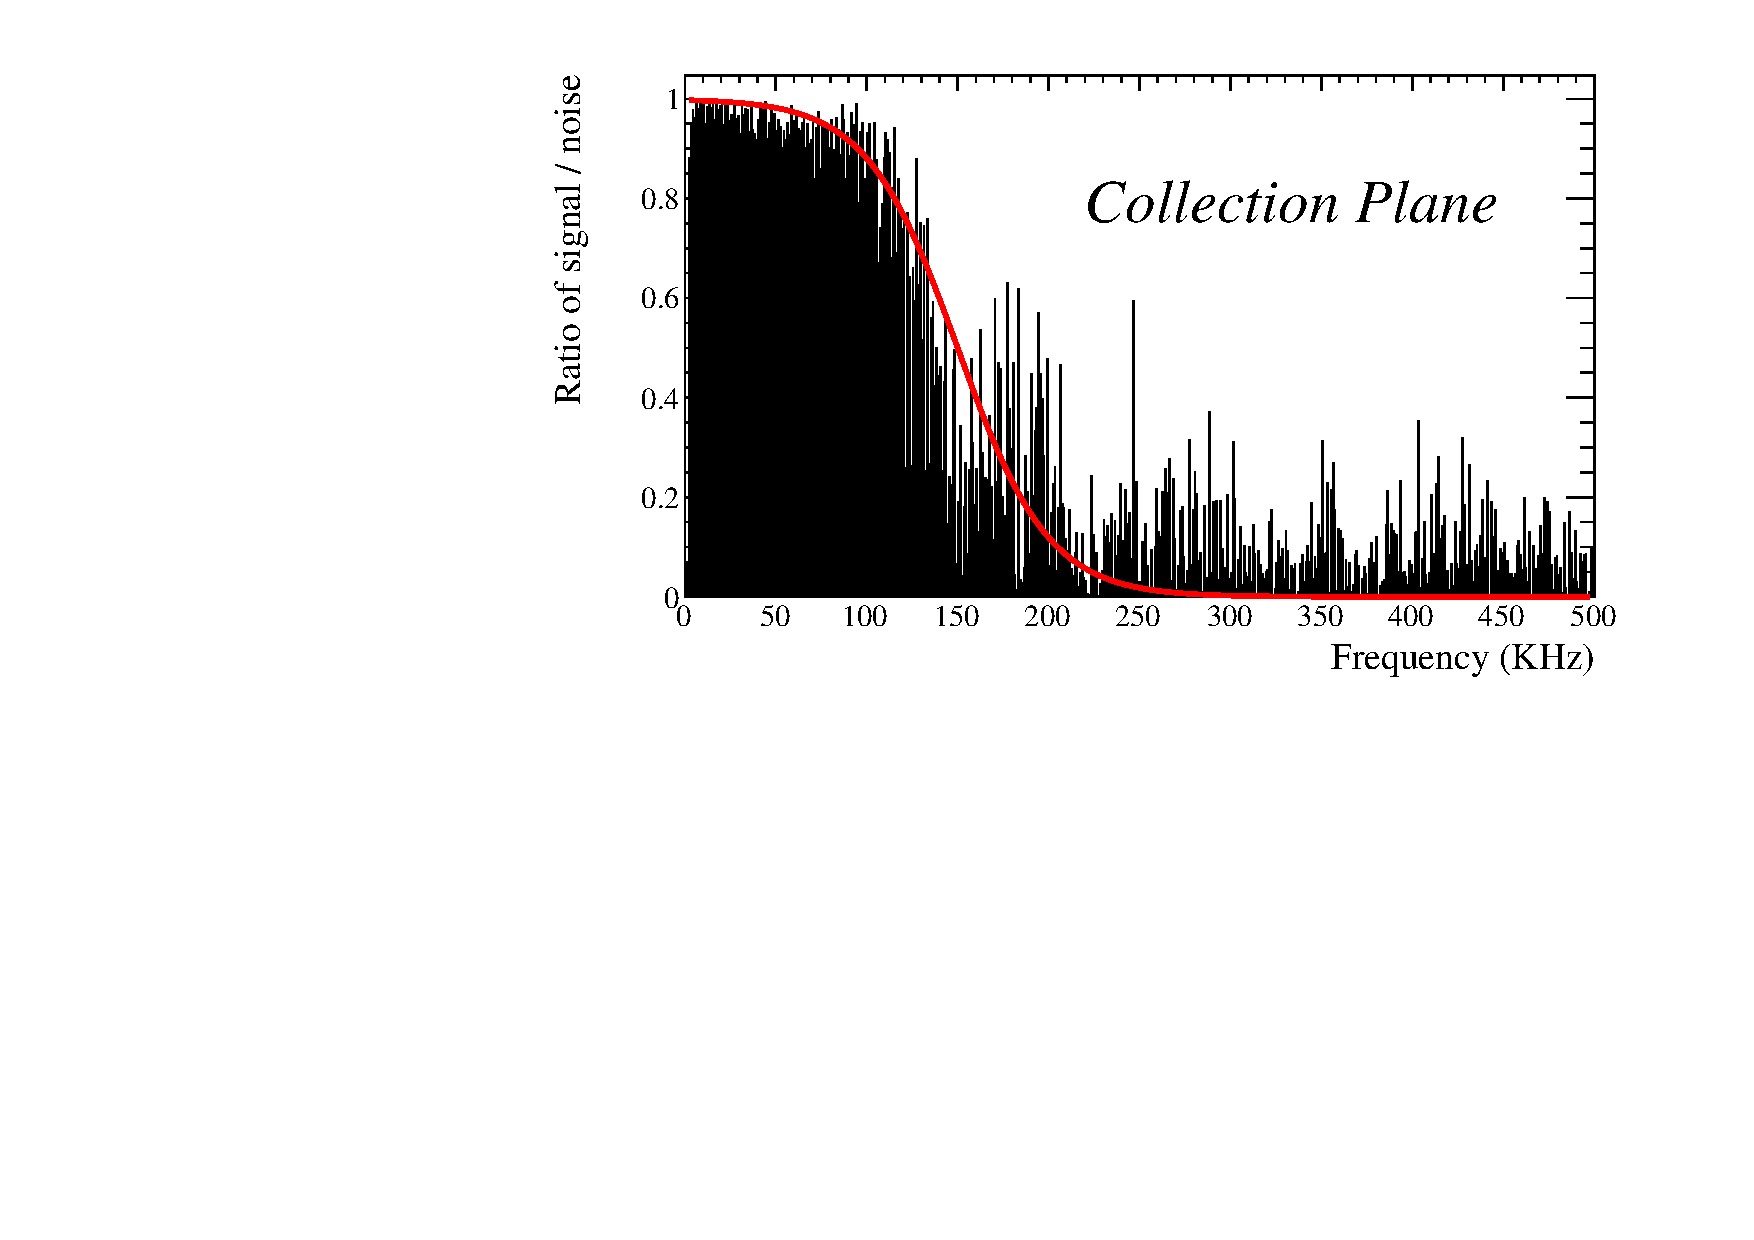
\includegraphics[width=\textwidth]{Collection}
    \caption{The $signal/noise$ ratio for a collection plane wire, the red line shows the fraction of frequency power which passes the filter.}
    \label{fig:FreqCollection}
  \end{subfigure}
  \hspace{0.08\textwidth}
  \begin{subfigure}{0.45\textwidth}
    \centering
    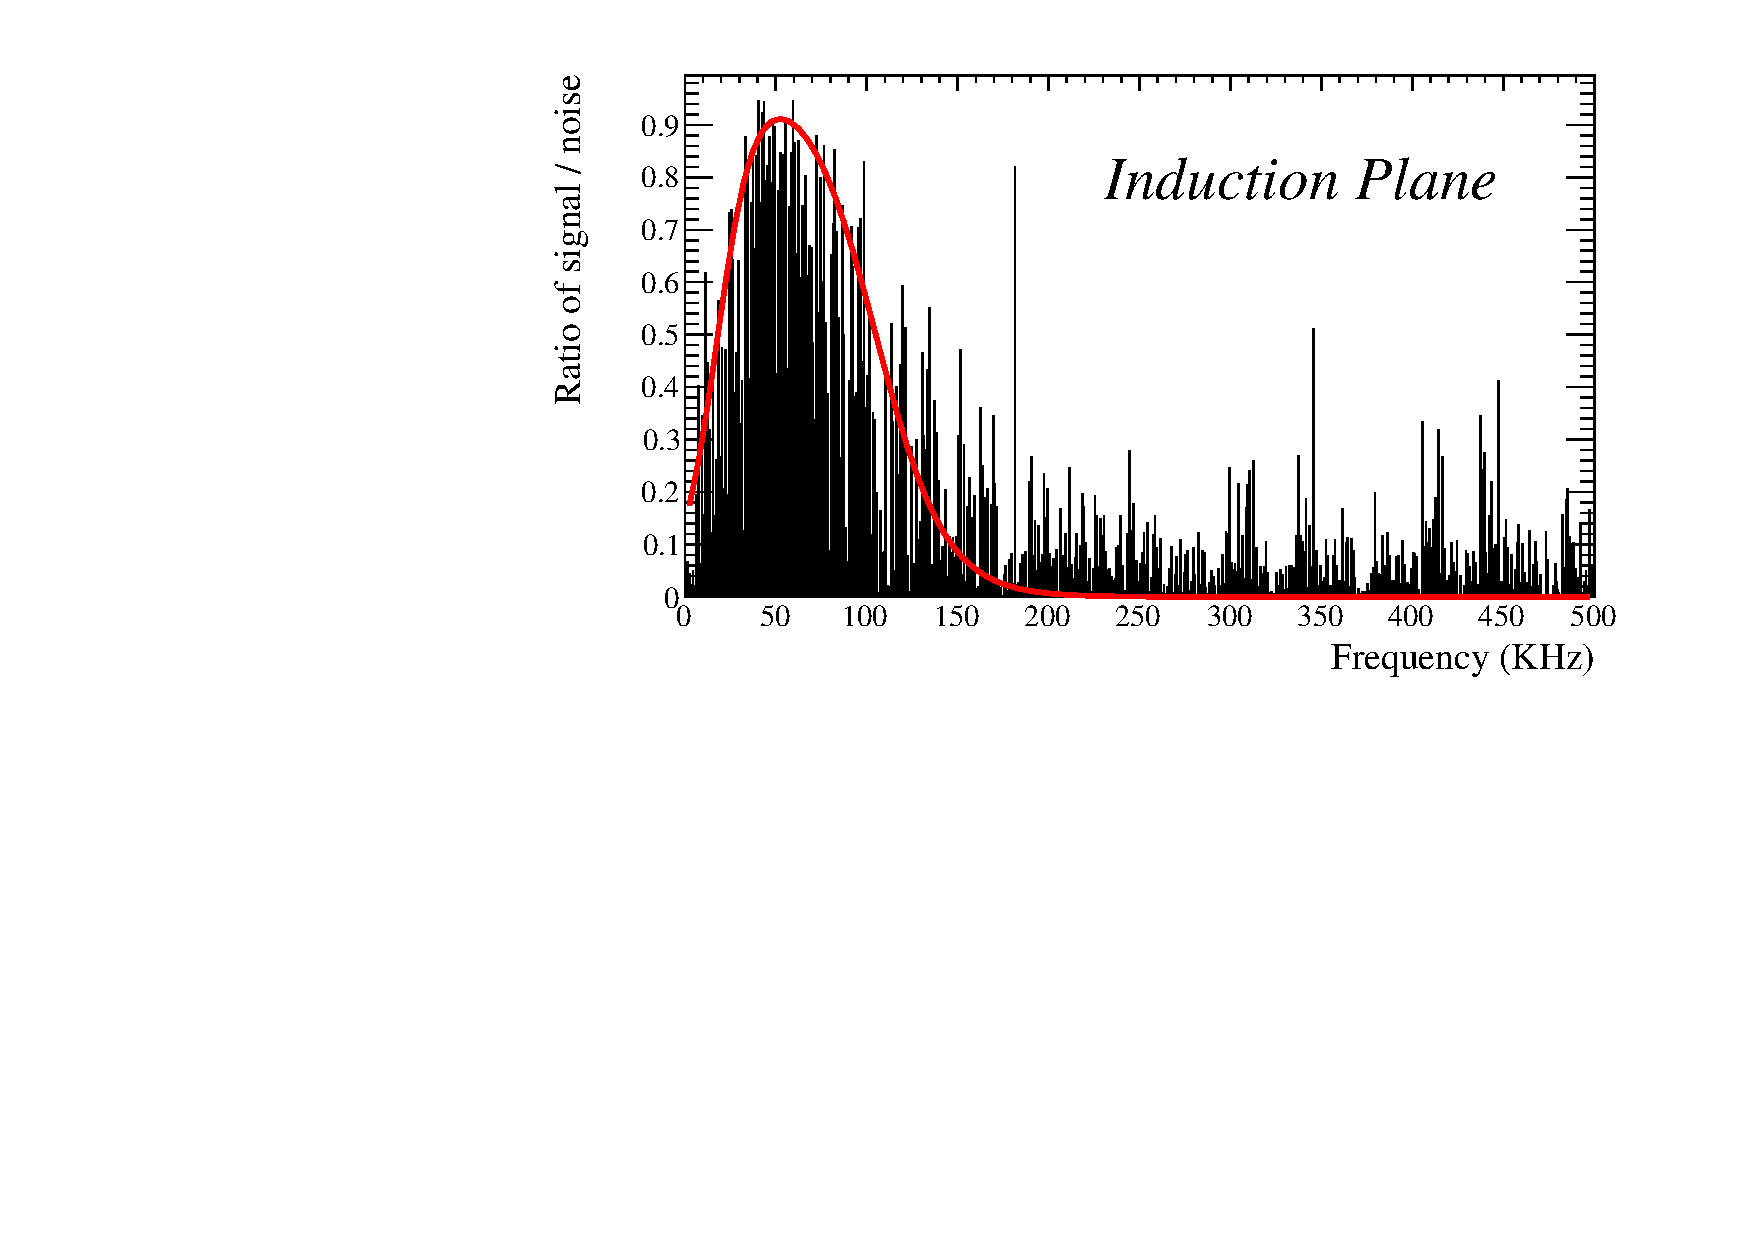
\includegraphics[width=\textwidth]{Induction}
    \caption{The $signal/noise$ ratio for an induction plane wire, the red line shows the fraction of frequency power which passes the filter.}
    \label{fig:FreqInduction}
  \end{subfigure}
  \caption[Applying Wiener filters to the 35 ton data]{The application of Wiener filters to the 35 ton data.}
  \label{fig:FrequencyFilter}
\end{figure}

An example of the effect of the noise mitigation steps is shown in Figure~\ref{fig:NoiseRemoval}, where the left side shows the raw data and the right side shows the data after the stuck code unsticker, coherent noise removal and Wiener filter algorithms have been applied after the removal of the most noisy wires. \\

\begin{figure}[h!]
  \centering
  \begin{subfigure}{0.45\textwidth}
    \centering
    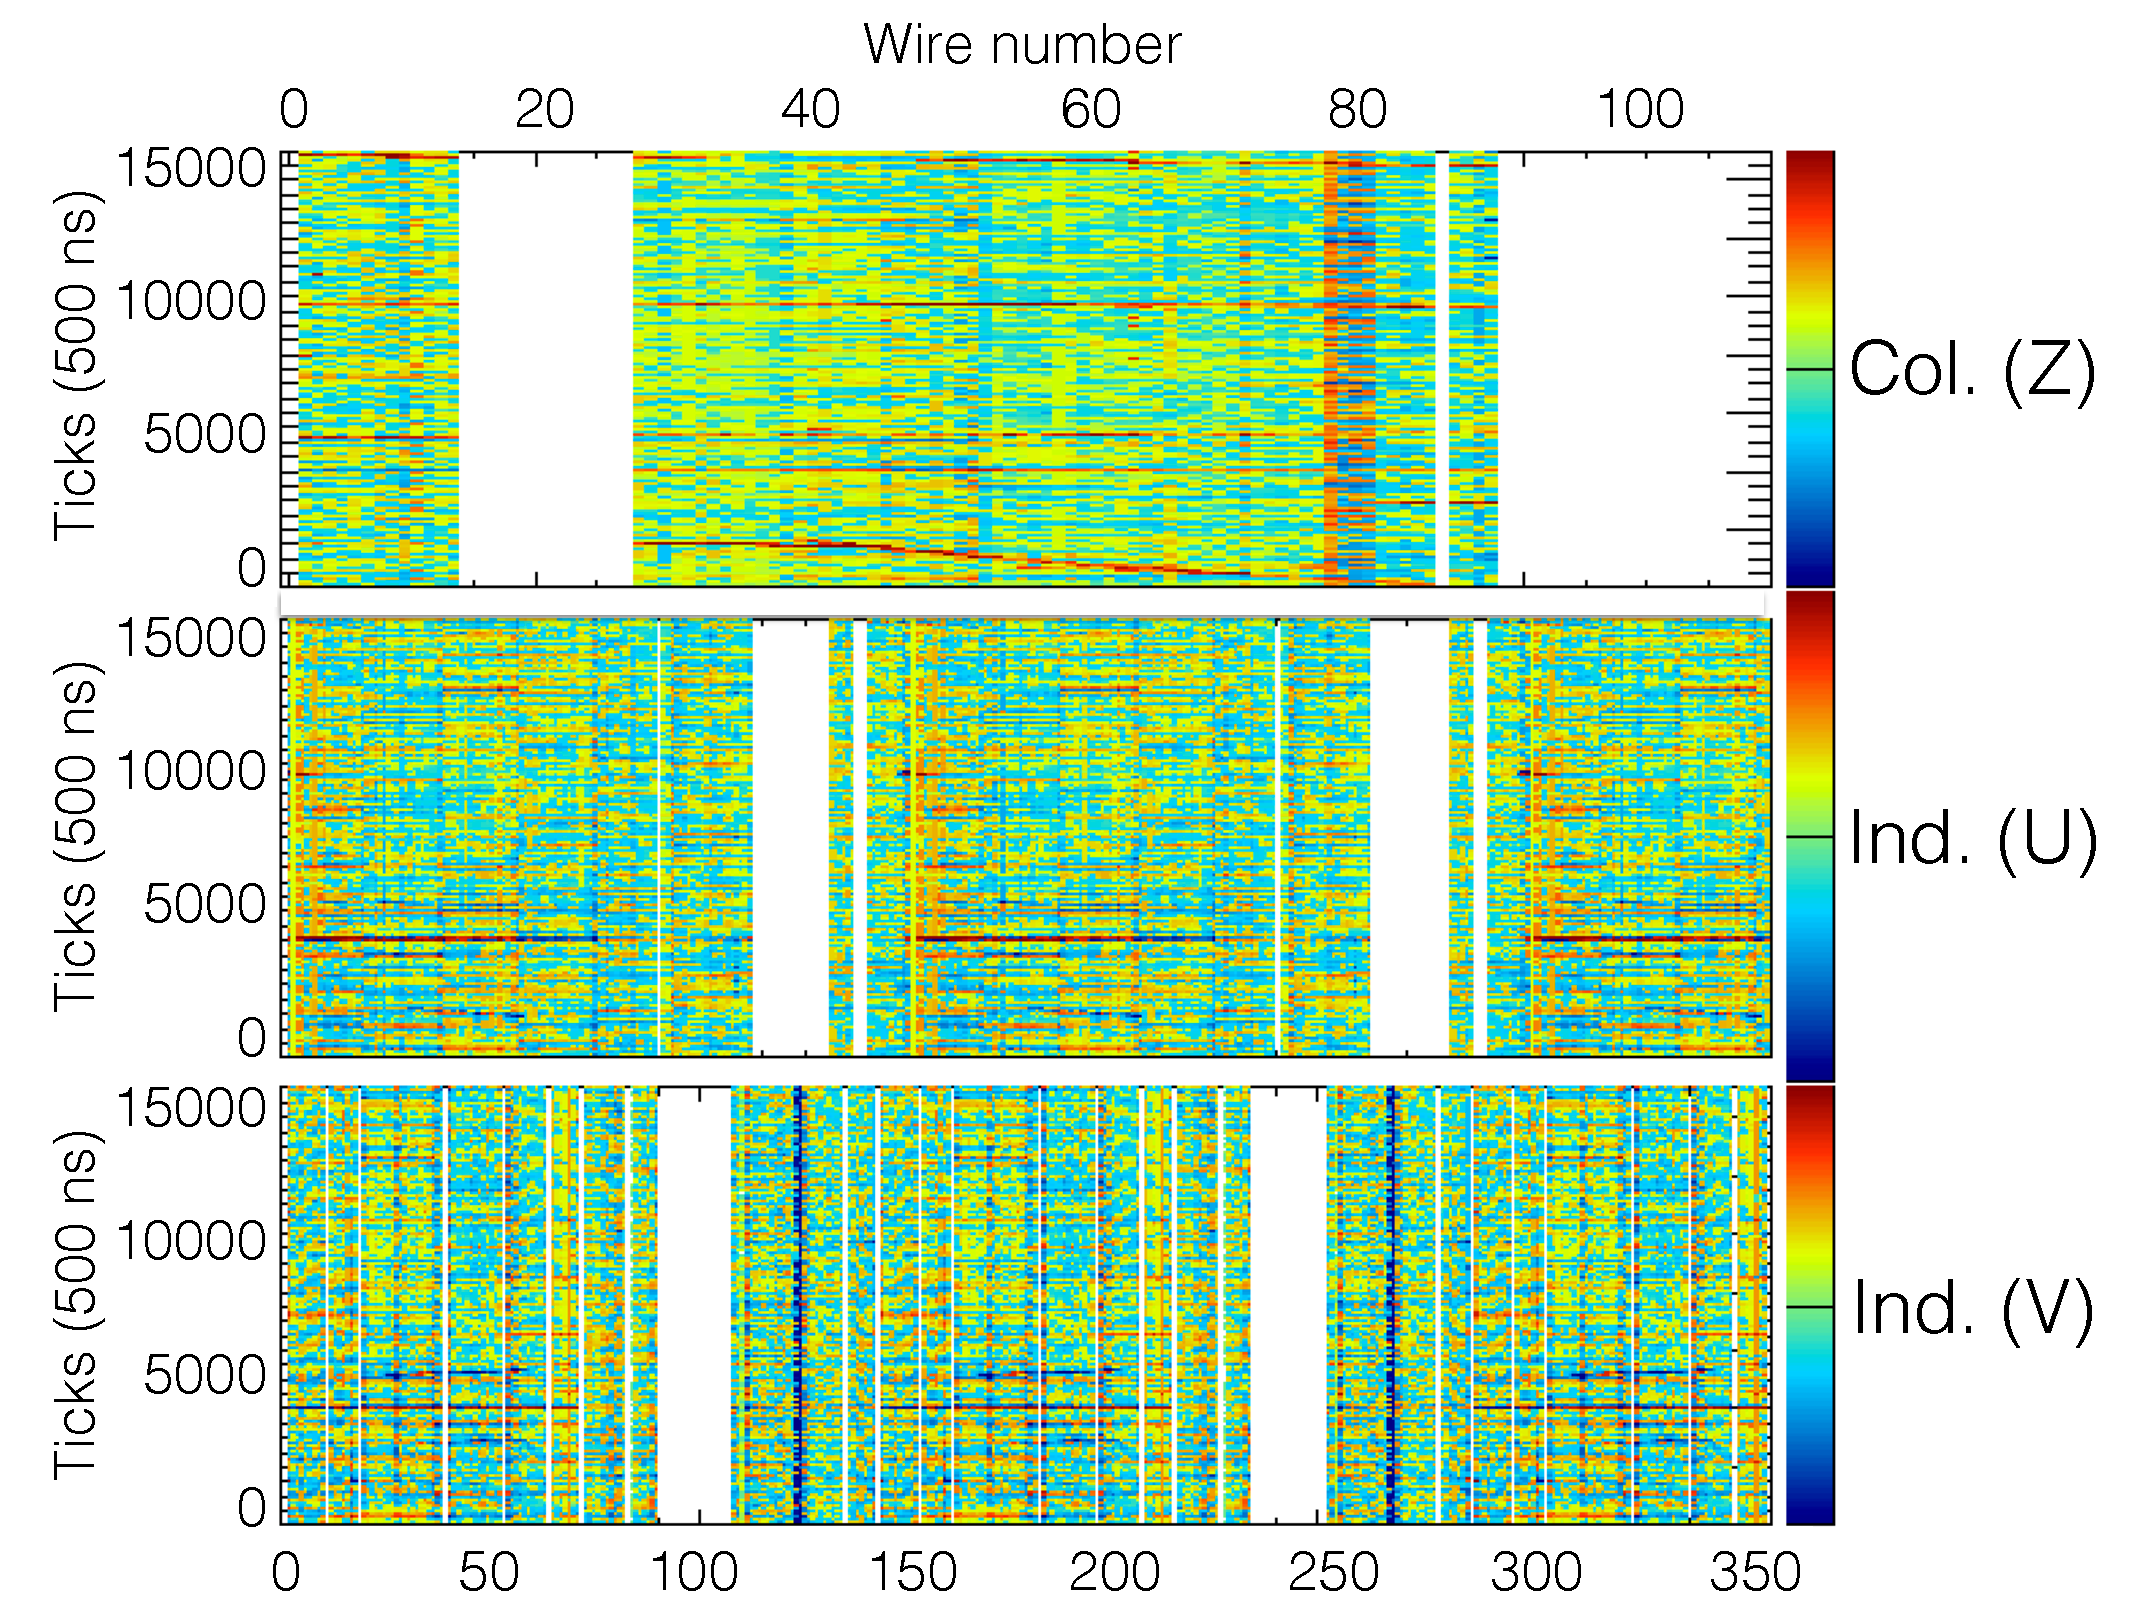
\includegraphics[width=\textwidth]{Evd_BeforeNoise}
    \caption{Raw signal before noise removal}
  \end{subfigure}
  \hspace{0.08\textwidth}
  \begin{subfigure}{0.45\textwidth}
    \centering
    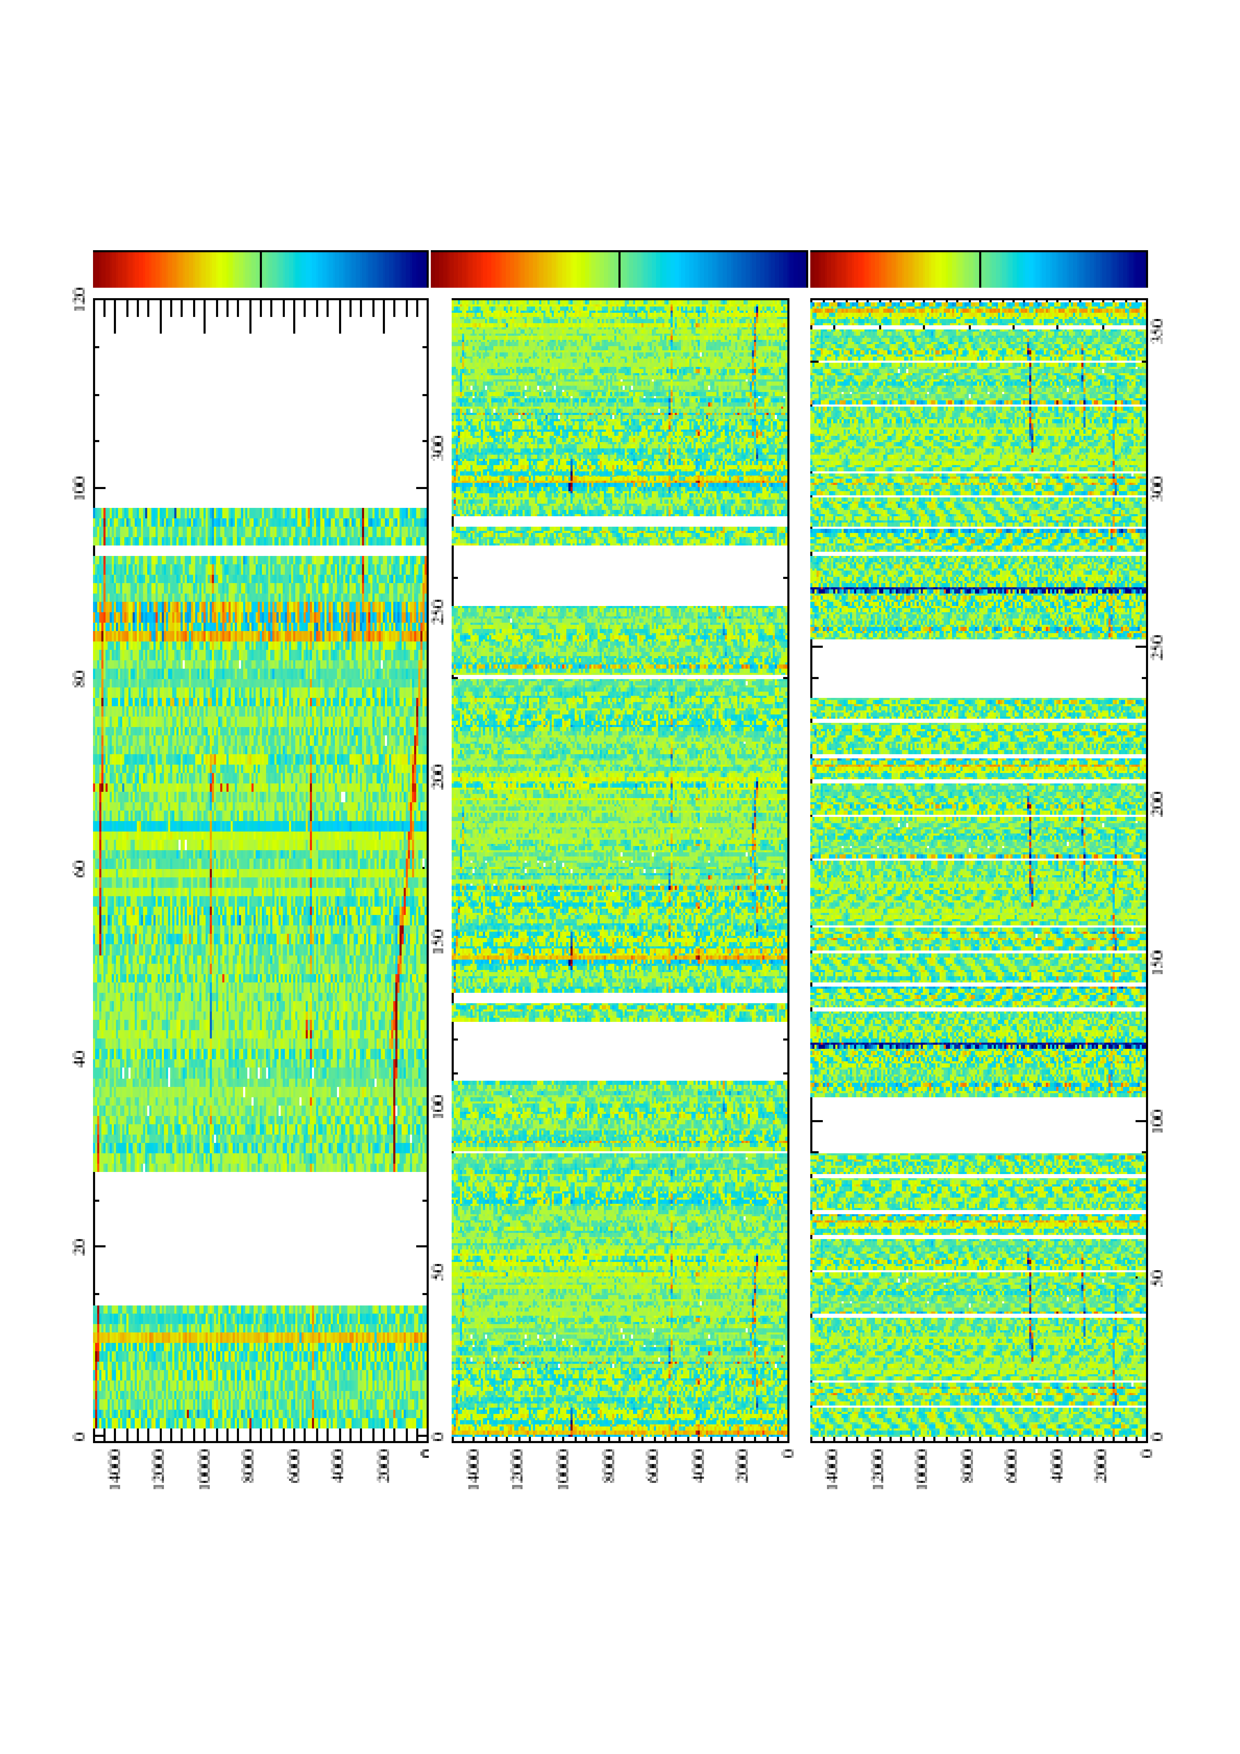
\includegraphics[width=\textwidth]{Evd_AfterNoise}
    \caption{Signal after noise removal}
  \end{subfigure}
  \caption[The effect of noise removal algorithms in the 35 ton]{Event displays showing the effect of the noise removal algorithms on data in the 35 ton.}
  \label{fig:NoiseRemoval}
\end{figure}

Transitions to a higher noise state associated with strong signals at high frequencies, between 400 and 650 KHz, were observed after cool down. The transitions would occur approximately every 2 hours and were occasionally observed to happen shortly after a saturation event across the whole detector \citep{35tonNoiseMeeting}. Once the state was induced the only way to stop it was to power cycle the low voltage supplies. It was found that power cycling APA3 could both stop and induce the higher noise state, importantly this was the only APA with electronics located at the base of the TPC. The data taken during the elevated noise state was unrecoverable as the electronics noise was too large, and so upon the observation of a transition the low voltage supplies were power cycled. It was observed that the transitions occurred much less frequently when APA3 was not powered and so it was not used for significant portions of the data taking period. Despite efforts to study the transitions during warm testing they were unable to be induced and have not been observed in other experiments such as MicroBooNE despite using the same low voltage supplies. It is thought that the cause of the transitions is a feedback loop in the low voltage cable which was much longer in the 35 ton than in MicroBooNE, this would explain why APA3 was more susceptible as the cable is routed past its electronics~\citep{35tonNoiseDoc}.

%********************************** % Fourth Section  *************************************
\section{Performance of reconstruction algorithms} \label{sec:DataAlgs}  %Section - X.4
Following the noise removal outlined above hit and track finding was still more difficult than in simulations due to the still elevated noise level. In order for a sensible number of hits to be reconstructed the hit finding threshold had to be substantially increased in data as compared to Monte Carlo, this meant that many of the low energy hits would not be reconstructed. \\

A potential solution to not reconstructing the low energy hits is to use the counter positions to select only hits which could have caused co-incidences. When determining whether a reconstructed hit could have caused the counter co-incidence a two-dimensional window around the counter edges in the YZ plane is constructed and timing information is used to extend this to three dimensions.  The $x$ position of the hit can be calculated using the hit time and electron drift velocity using Equation~\ref{eq:HitTime}. \\

Determining whether collection plane hits are within the counter window is trivial as they have a constant Z position and either cover the full detector height (tall APAs) or roughly half of the detector height (short APAs). The wrapping of the induction planes however means that each wire segment has to be considered individually and that multiple segments of a given wire could lie within the counter shadow. Choosing between these potential wire segments is done by iterating through the following steps. If at any point only one segment satisfies the condition then this segment is chosen:
\begin{itemize}
\item Does the wire segment intersect any collection plane wires which record hits?
  \begin{itemize}
  \item This is because when there is a signal on an induction plane there should also be signals on the collection wires.
  \end{itemize}
\item Are there adjacent wires which have hits at a similar time?
  \begin{itemize}
  \item This is because one would expect a track to deposit energy on multiple adjacent wire segments. 
  \end{itemize}
\item Which hit lies closest to the line defined by unique collection plane hits in the XZ plane?
  \begin{itemize}
  \item This is follows identical logic to the first criteria, but selects the hit which best matches the collection plane hits and attempts to remove the effect of noisy collection plane wires by only using wires which have one hit within the counter shadow. This would also hopefully improve the quality of the fit as there will not be numerous outlying hits.
  \item This can be changed to consider the line defined by previously selected hits in the given TPC and plane where the hit choices are.
  \end{itemize}
\end{itemize}
%DO I WANT SOME SORT OF FIGURE SHOWING THIS? LOTS OF HITS -> ONLY TRACK HITS? COL HITS USED IN ITEM 3, OVERLAYED WITH ALL INDUCTION PLANE HITS CONSIDERED, WITH THE ONES KEPT IN A DIFFERENT COLOUR? \\

Following a re-optimisation of the clustering algorithms it was observed that the standard reconstruction could achieve track reconstruction to a similar efficiency as the counter shadowing and so the standard reconstruction has been used in the discussions to follow \citep{TingjunClustering}. There has since been an effort to improve the counter shadowing hit disambiguation to remove the outlying collection plane hits using the MLESAC method \citep{MLESAC} whereby points which are far away from a best fit are ignored, these studies are still on-going~\citep{MattMLESAC}. \\

%****** Now to talk about the reconstruction efficiencies... ******%
A symptom of the elevated noise state is that signals are often dropped on one of the induction planes, this means that the tracking algorithms often have to combine clusters in only two of the three planes. Reconstruction using two planes was shown to be effective by the ArgoNeuT collaboration \citep{ArgoNeuT} so the loss of signal in one of the three planes is not prohibitive to track reconstruction. Another consequence of the elevated noise level is that even when the counters are used to seed hit finding the hit finding threshold is too high to reconstruct the very lowest hits. This causes the plot of $dQ/dx$ for muons, shown in Figure~\ref{fig:TingjunLifetime}, to look flat due to a cutoff at 100 ADC cm$^{-1}$ below which no hits are found. The inability to reconstruct the lowest energy hits means that calorimetry is all but impossible on the 35 ton dataset even though the tracking algorithms perform relatively well. \\

\begin{figure}[h!]
  \centering
  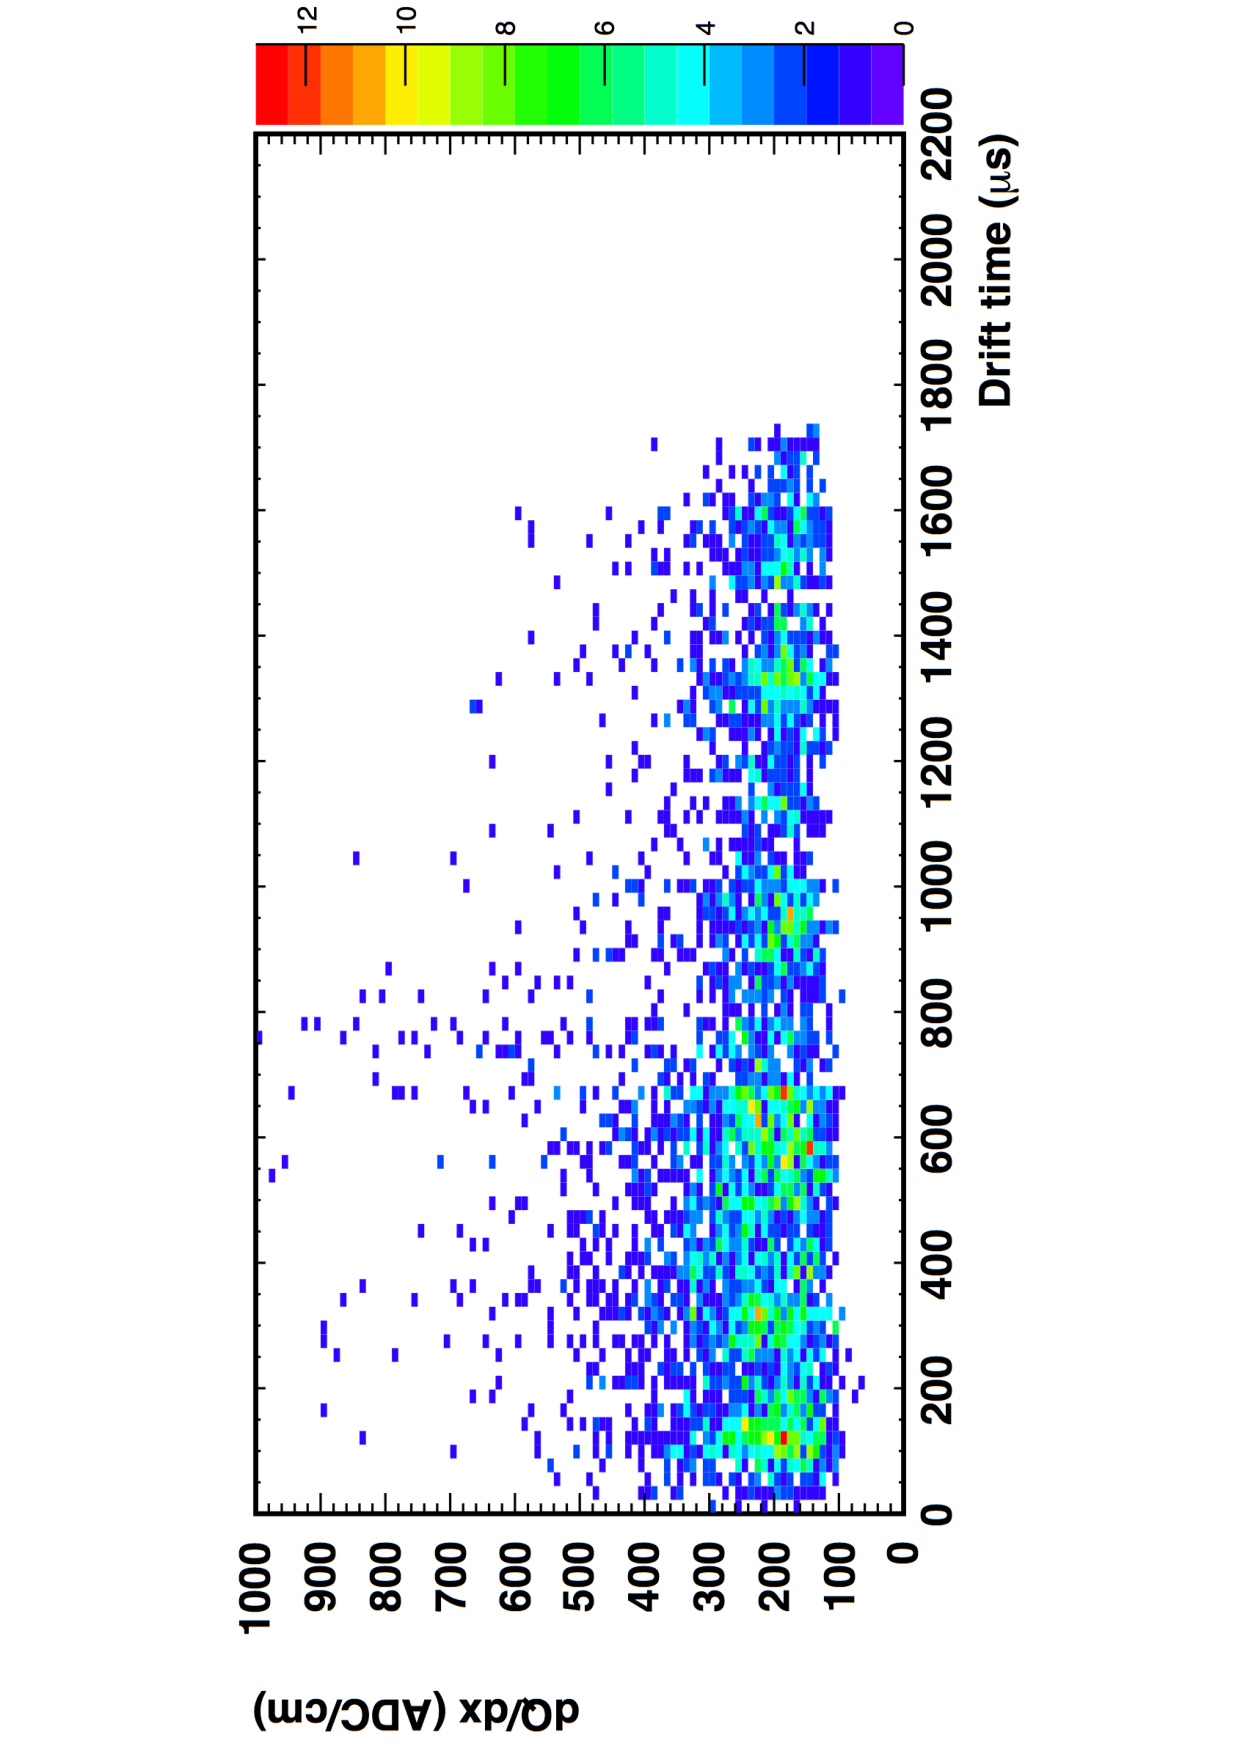
\includegraphics[width=0.85\textwidth]{TingjunLifetime}
  \caption[$dQ/dx$ in the 35 ton as a function of drift time]
          {The $dQ/dx$ values for a sample of muon collection plane hits \citep{TingjunLifetime}, note the cutoff at 100 ADC cm$^{-1}$ due to the hit finding threshold.}
  \label{fig:TingjunLifetime}
\end{figure}  

The inability to perform reliable calorimetry en masse means that the only particles which can be assuredly identified are the muons which triggered the counter co-incidences, making the analysis proposed in !!FIXME!!Section~ref{PIDAnalysis}!!FIXME!! extremely difficult if not impossible. The muons in the triggered sample will all traverse the detector but their orientations can be carefully selected by the user, for example one could easily select a sample of muons which cross the APAs at increasing angles, or are parallel to the wire planes at increasing drift distances. A reconstructed track is assigned to a given counter co-incidence if the dot product of the track and the co-incidence is more than 0.98 and the hit times are consistent with the $x$ positions of the counters, as shown in Figure~\ref{fig:CounterCoincidence}. This should result in a pure sample of tracks as parallel muons are unlikely to be highly correlated in time and any tracks reconstructed from the noise will have random directions and so will not pass the dot product cut. This is shown in data where if multiple tracks pass the dot product cut they are co-linear and are not randomly orientated, as shown in Figure~\ref{fig:CounterTrackAngle}. \\

\begin{figure}[h!]
  \centering
  \begin{subfigure}{0.45\textwidth}
    \centering
    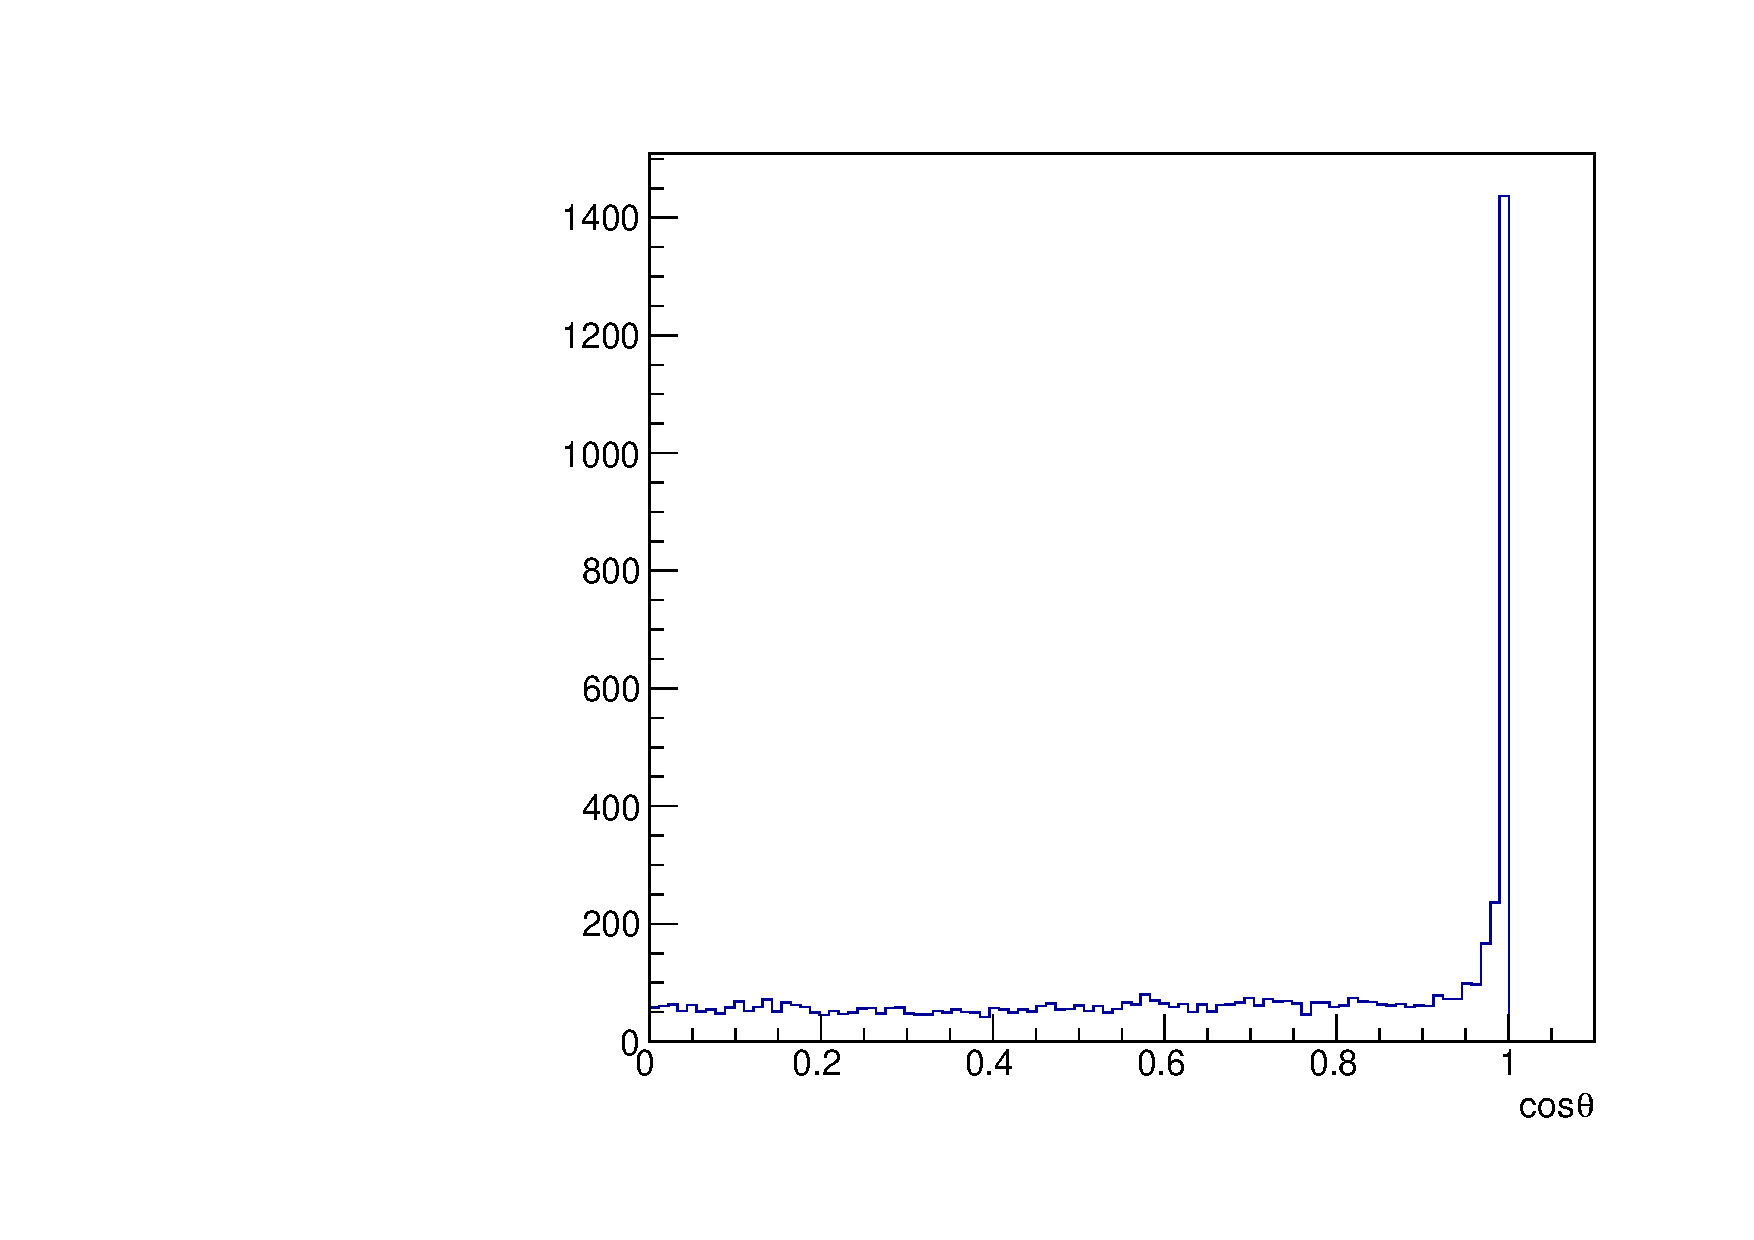
\includegraphics[width=\textwidth]{CosTheta_Data}
    \caption{All dot product values.}
  \end{subfigure}
  \hspace{0.08\textwidth}
  \begin{subfigure}{0.45\textwidth}
    \centering
    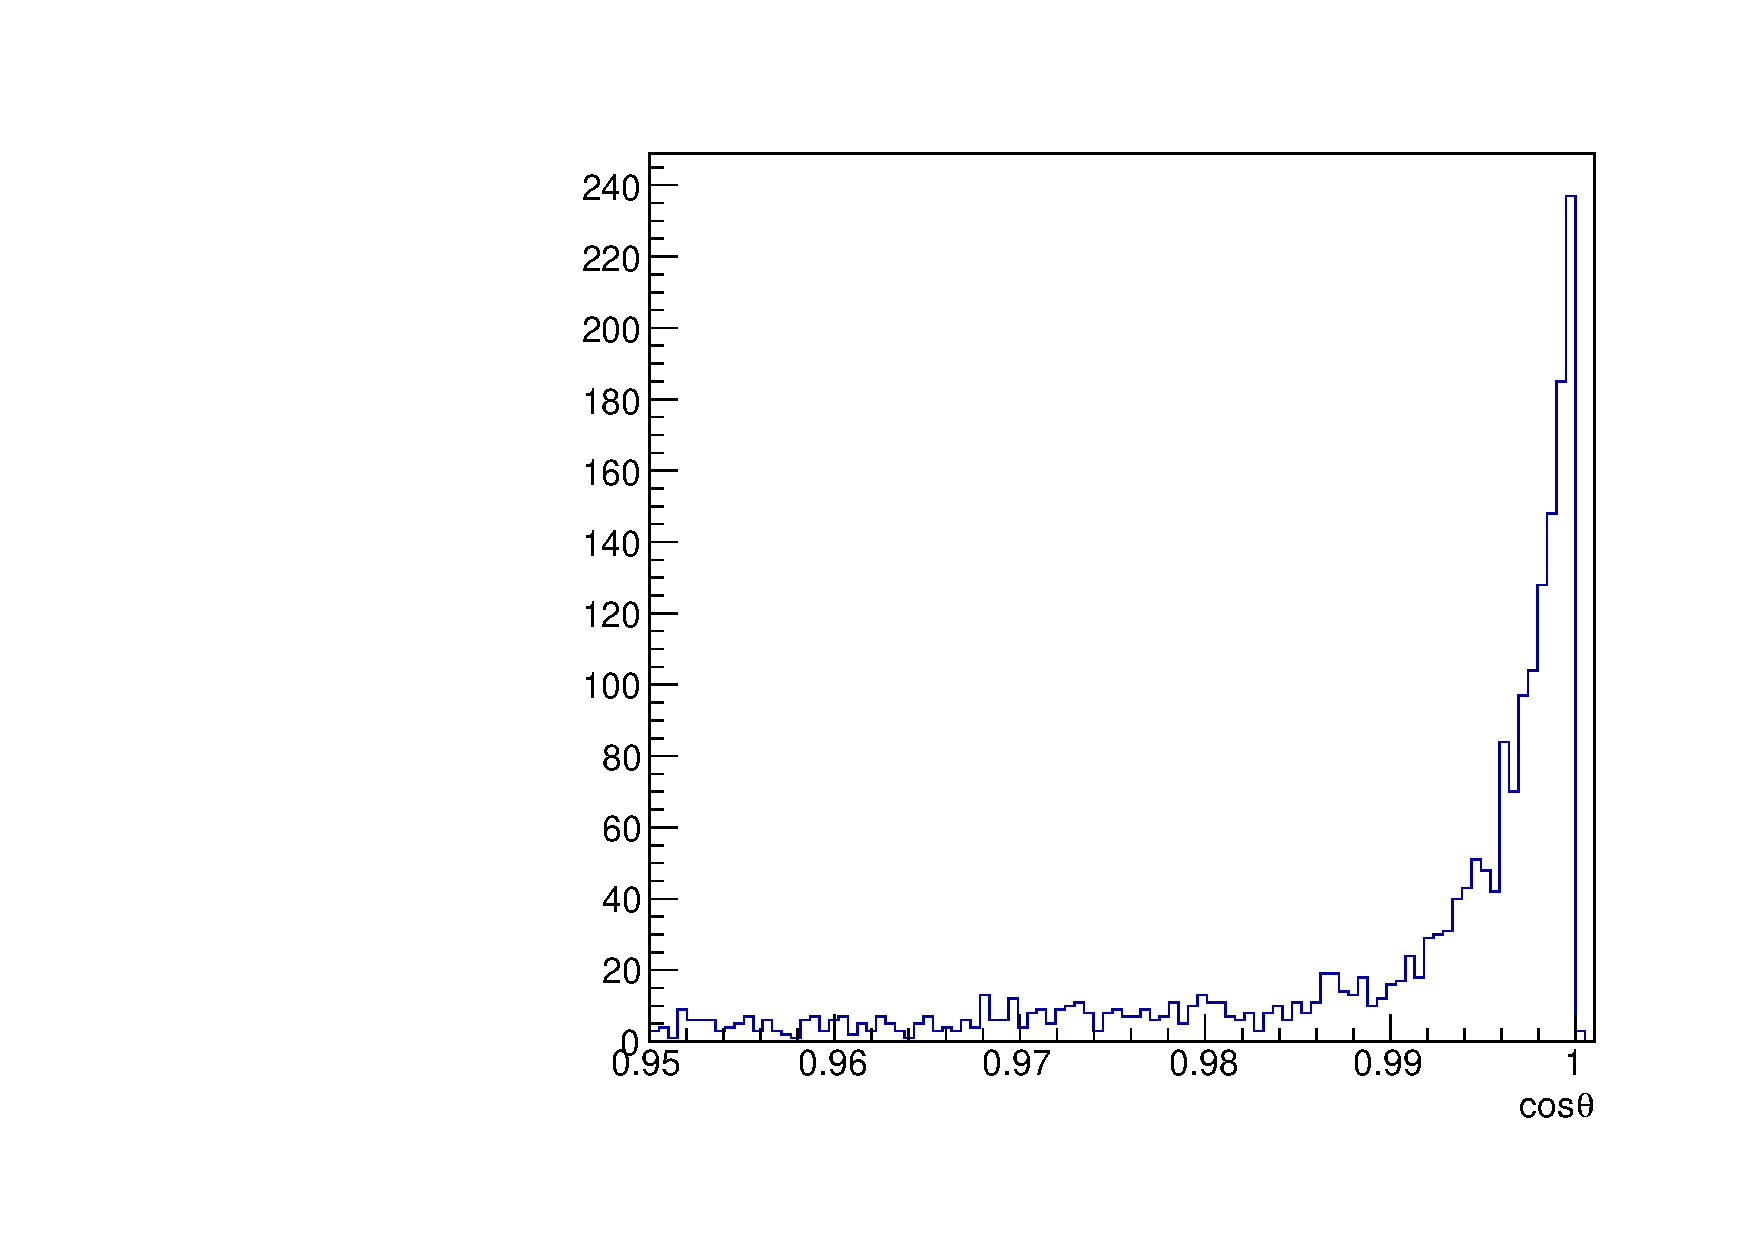
\includegraphics[width=\textwidth]{CosThetaZoom_Data}
    \caption{Dot product values close to 1.}
  \end{subfigure}
  \caption[The dot product of track and counter coincidences]
          {The dot product of track and counter coincidences.}
          \label{fig:CounterCoincidence}
\end{figure}

\begin{figure}[h!]
  \centering
  \begin{subfigure}{0.45\textwidth}
    \centering
    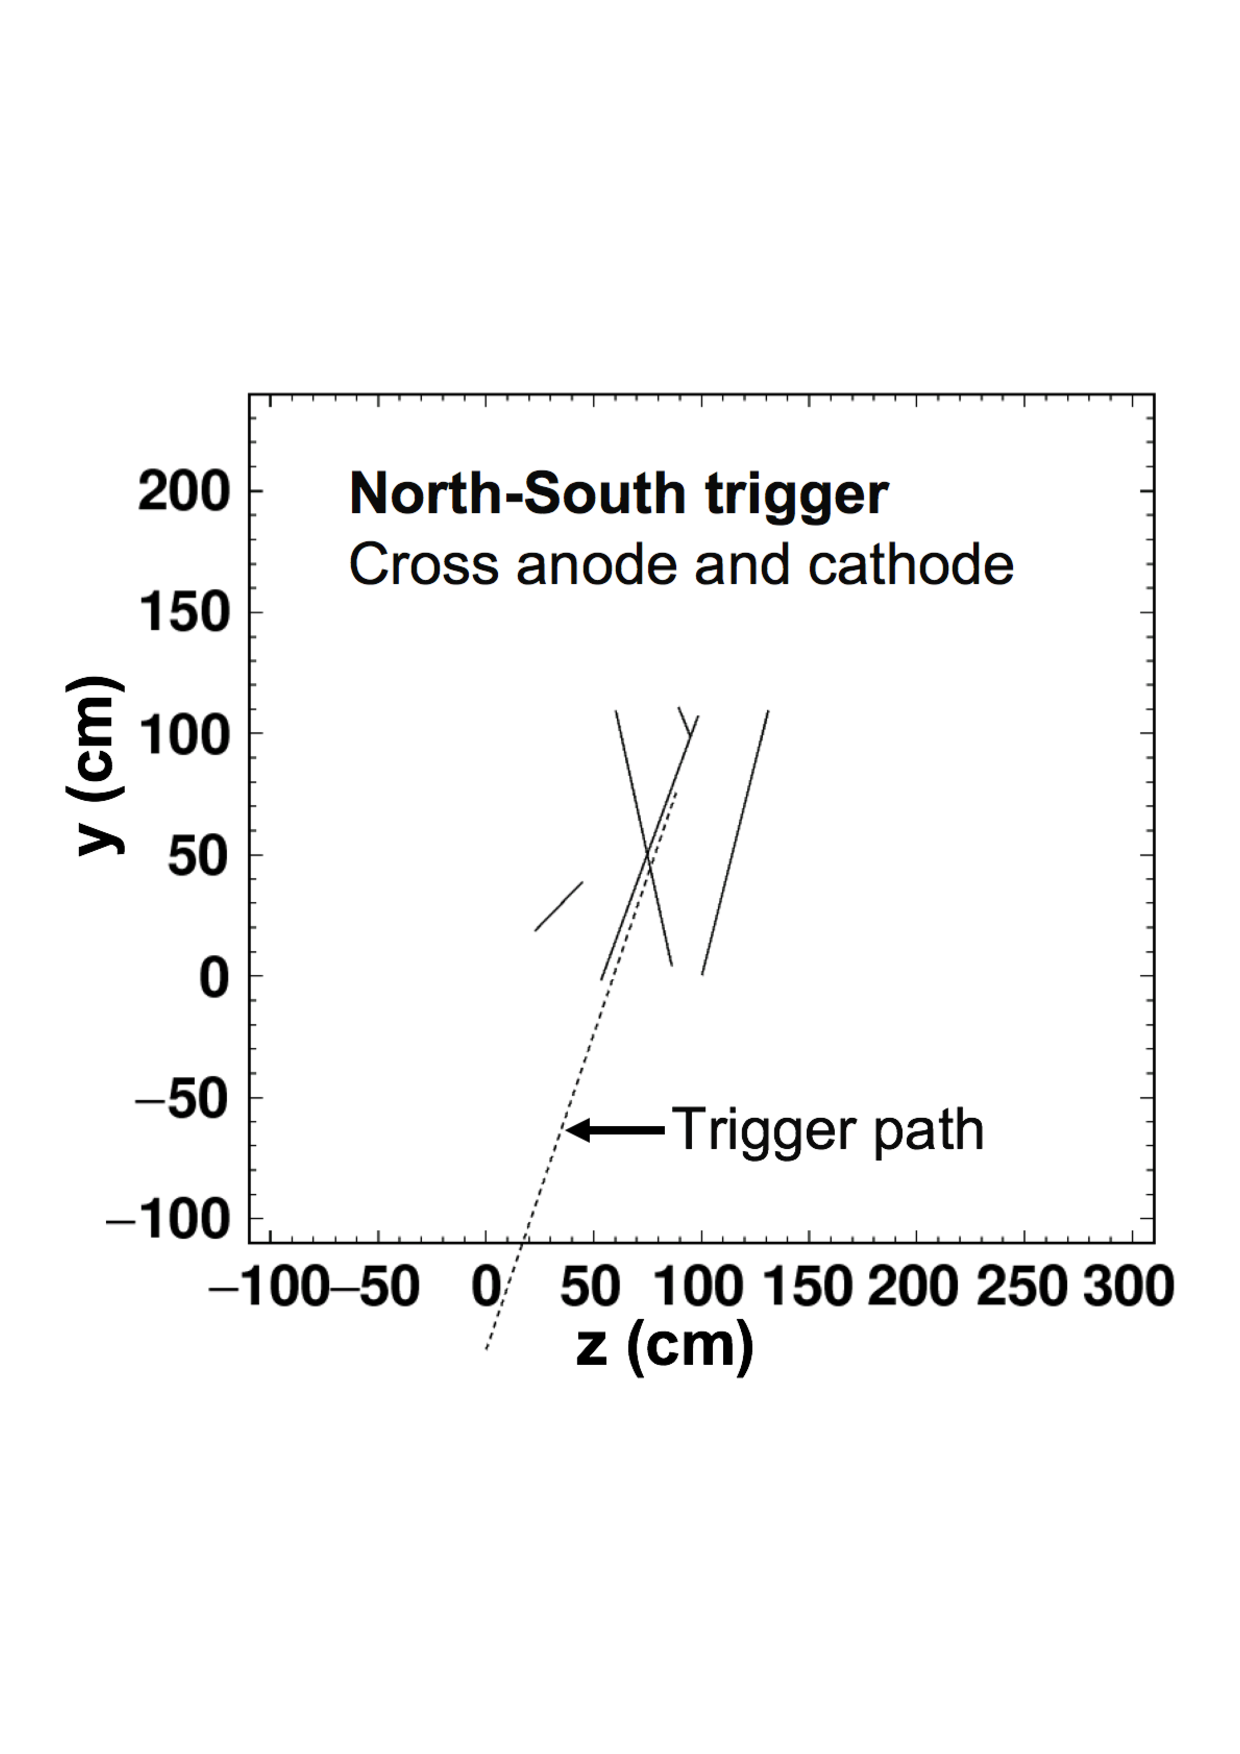
\includegraphics[width=\textwidth]{North-South}
    \caption{A North-South counter coincidence.}
  \end{subfigure}
  \hspace{0.08\textwidth}
  \begin{subfigure}{0.45\textwidth}
    \centering
    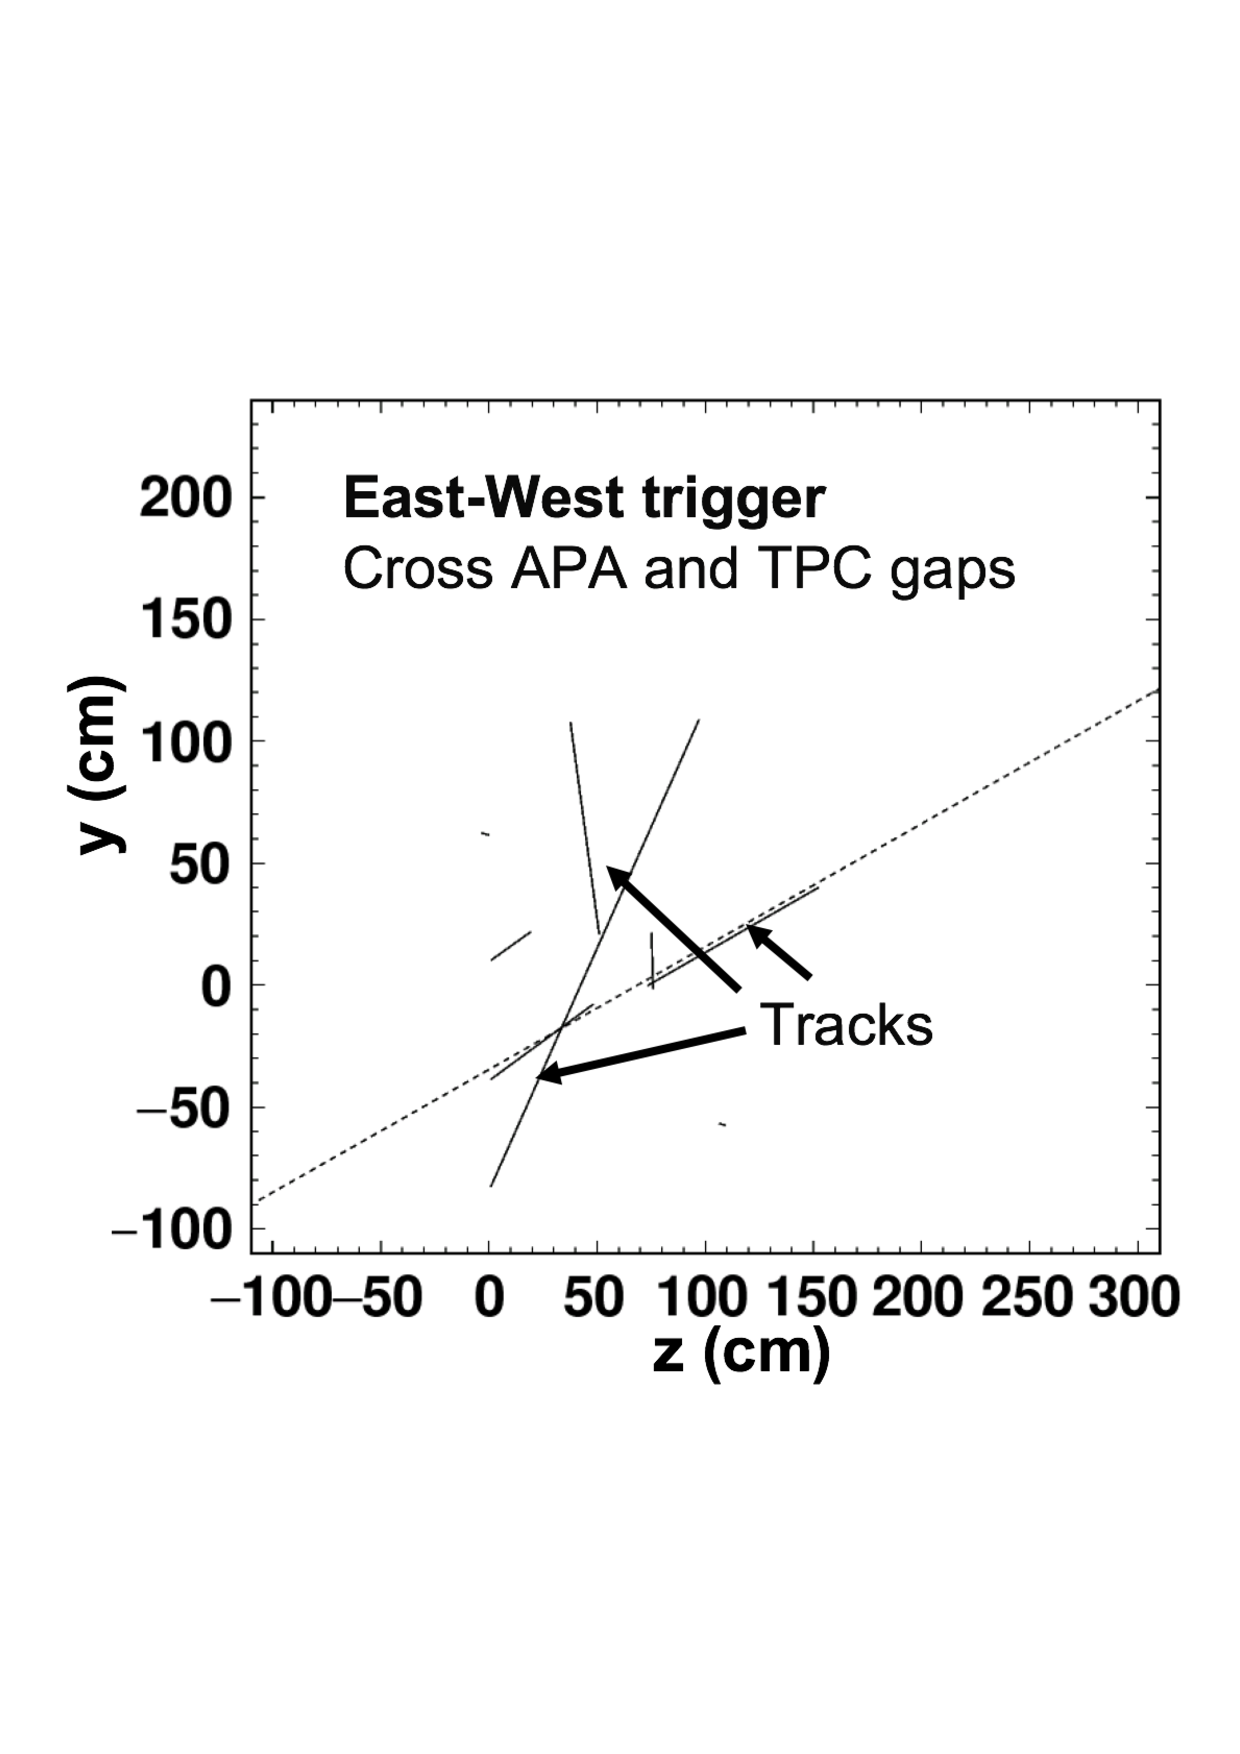
\includegraphics[width=\textwidth]{East-West}
    \caption{An East-West counter coincidence.}
  \end{subfigure}
  \caption[The alignment of tracks and counter coincidences]
          {The alignment of reconstructed tracks and the counter coincidences they cause.}
          \label{fig:CounterTrackAngle}
\end{figure}

By matching tracks in this way it possible to evaluate the reconstruction efficiencies for these muons at increasing drift distances and track angles. If multiple tracks are aligned with the coincidence and are within the expected time region then their track lengths are summed when calculating reconstruction efficiencies as it is expected that the track was split by a region of the detector either being turned off or too noisy to reliably reconstruct a track. A minimum reconstructed length of 50 cm is used to determine if the track was partially reconstructed as above this length the track is likely to have been stitched between TPCs, the verification of which was a design goal of the 35 ton. A reconstructed track that is 50 cm long is also likely to have a large number of hits on collection plane wires that are not noisy, these hits are needed when calculating purity or measuring the effect of diffusion as discussed in Section~\ref{DiffusionAnalysis}. \\

From Figure~\ref{fig:DataRecoEffics} it is evident that the reconstruction efficiency for tracks with shallow angles relative to the APAs is extremely poor, with the efficiency for tracks aligned with counter differences of 0 or 1 never rising above 10\%. This is due to the coherent noise removal where hits which are correlated in time will be removed as they will be perceived as being noise as opposed to real signals. When considering tracks aligned with counter differences of between 3 and 5 the reconstruction is seen to be perform reasonably well for tracks whose centres are less than 140 cm away from the APAs, before decreasing for tracks which have a longer drift distance. A decrease in reconstruction efficiency for tracks at large drift distances is due to the hits being below threshold and so not being reconstructed. It should be noted that in order to observe a drift distance effect on reconstruction efficiency the distance plotted is the average $x$ position of the counters, so a track going from 10 cm to 230 cm will have an average $x$ position of 120 cm (assuming a straight trajectory) as shown by the point for Counter difference 7 in Figure~\ref{fig:DistanceCanvas} with $\sim$23\% efficiency. \\

\begin{figure}[h!]
  \centering
  \begin{subfigure}{0.45\textwidth}
    \centering
    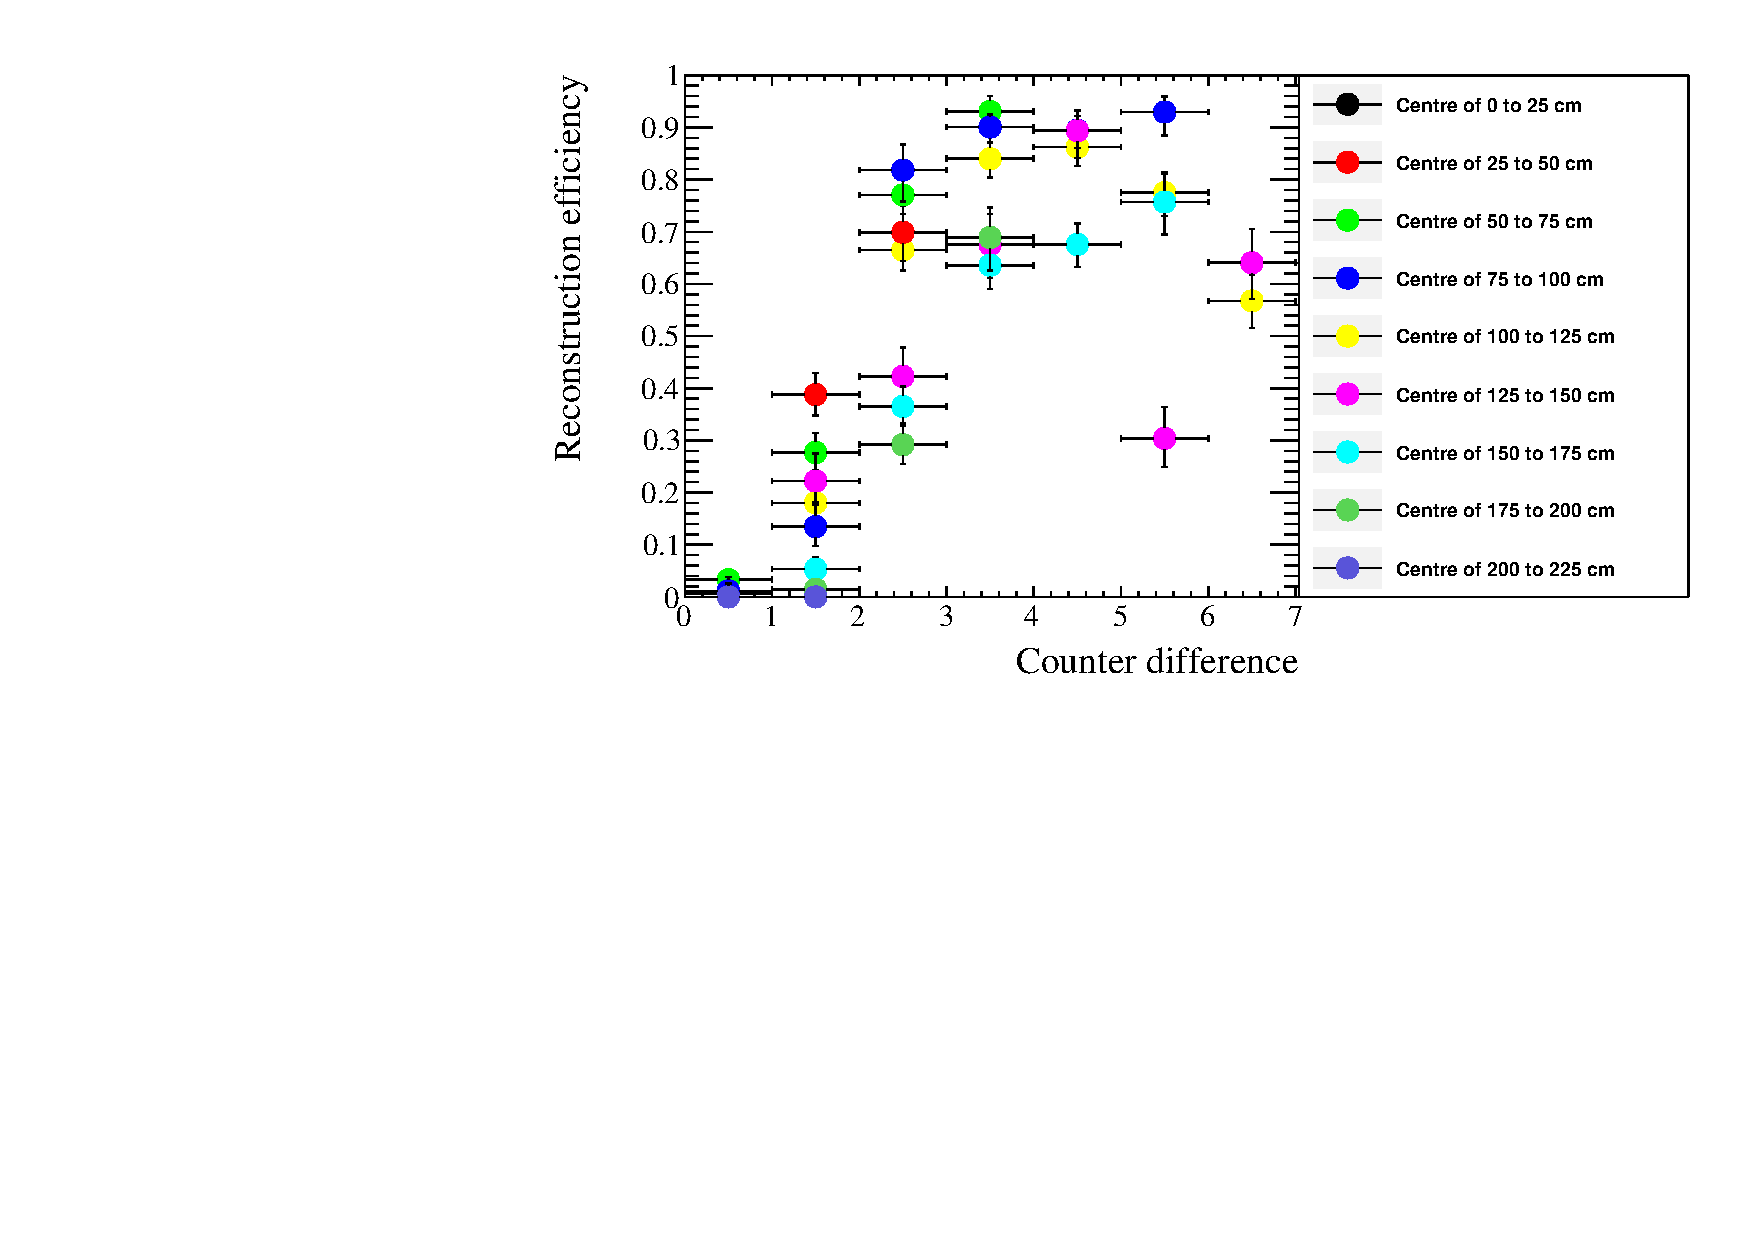
\includegraphics[width=\textwidth]{AngleCanvas_50}
    \caption{The difference in efficiencies of different track angles relative to the APAs plotted for increasing distance from the APAs.}
    \label{fig:AngleCanvas}
  \end{subfigure}
  \hspace{0.08\textwidth}
  \begin{subfigure}{0.45\textwidth}
    \centering
    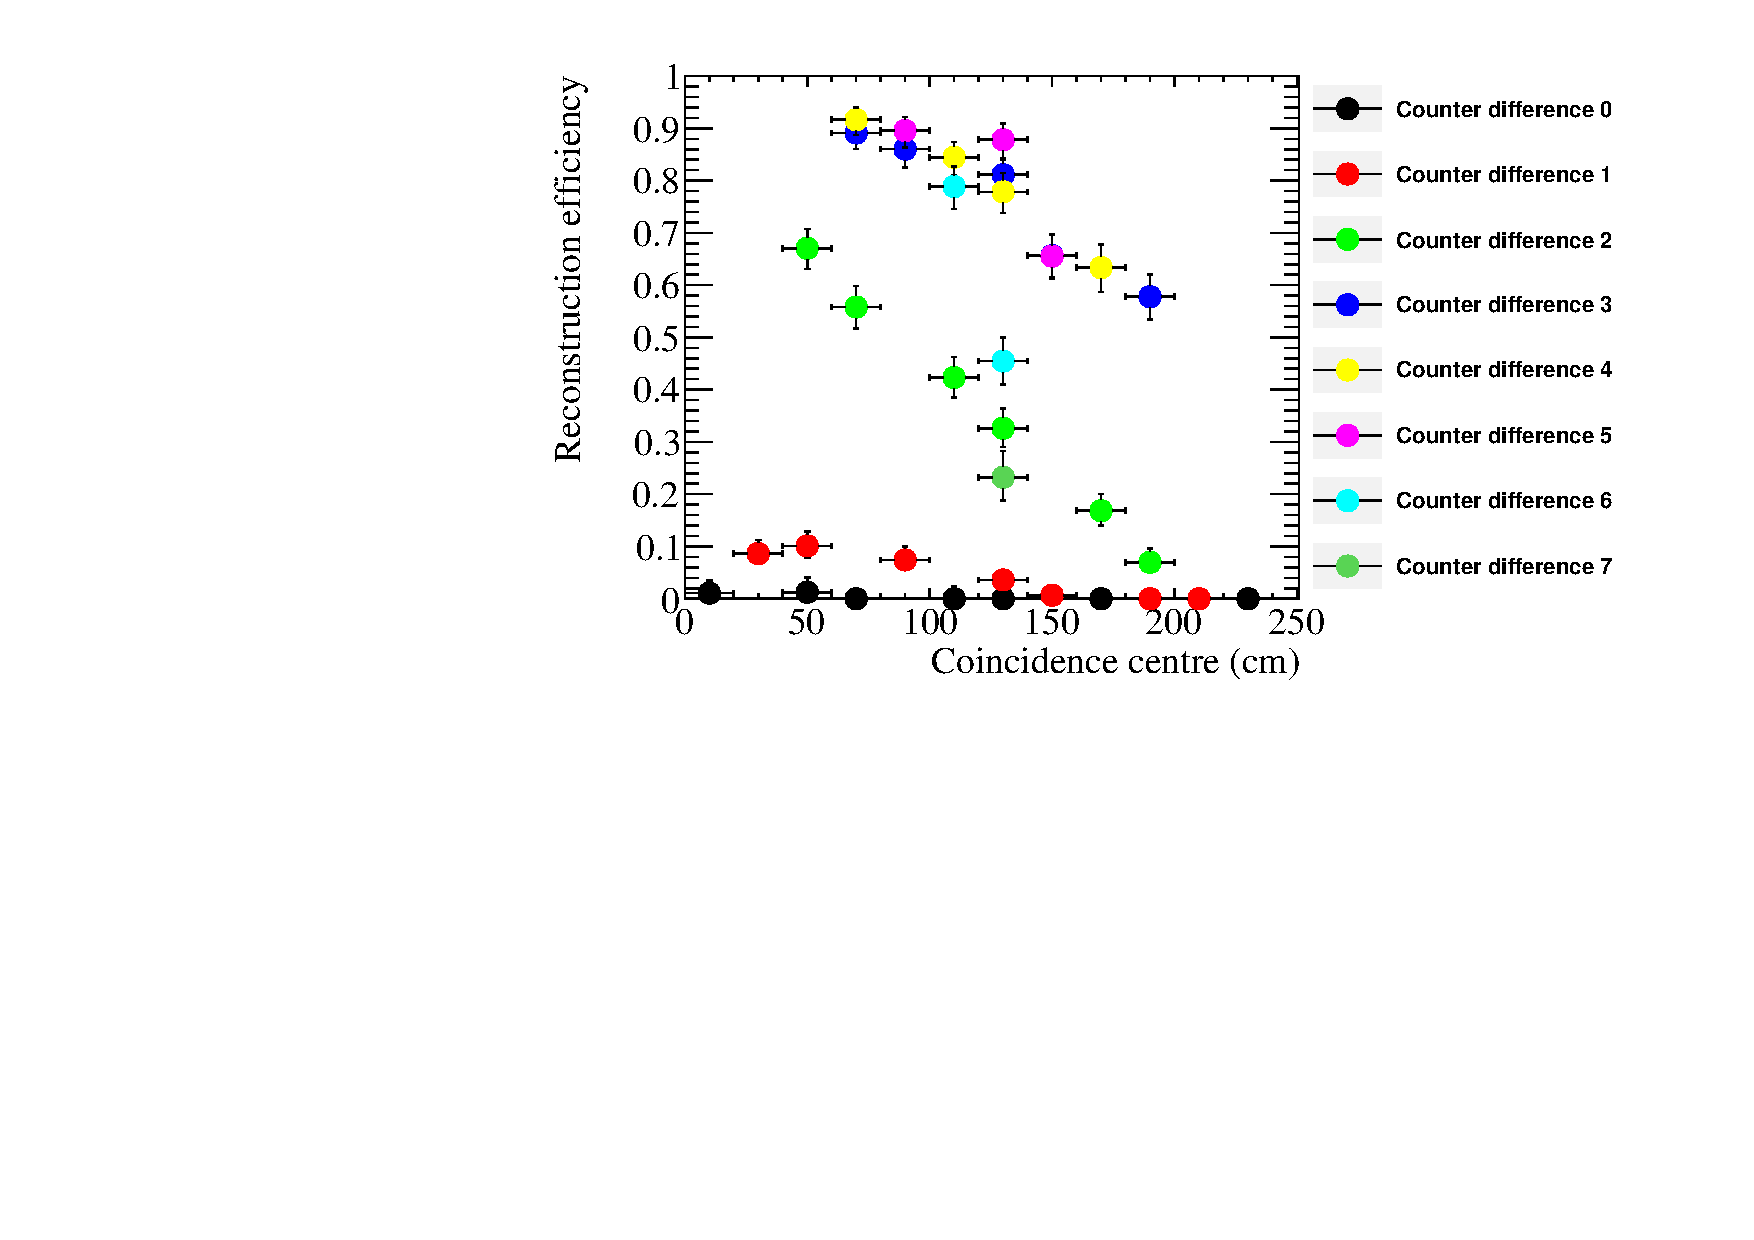
\includegraphics[width=\textwidth]{DistanceCanvas_50}
    \caption{The difference in efficiencies at increasing distances from the APAs plotted for increasing track angles relative to the APAs.}
    \label{fig:DistanceCanvas}
  \end{subfigure}
  \begin{subfigure}{0.45\textwidth}
    \centering
    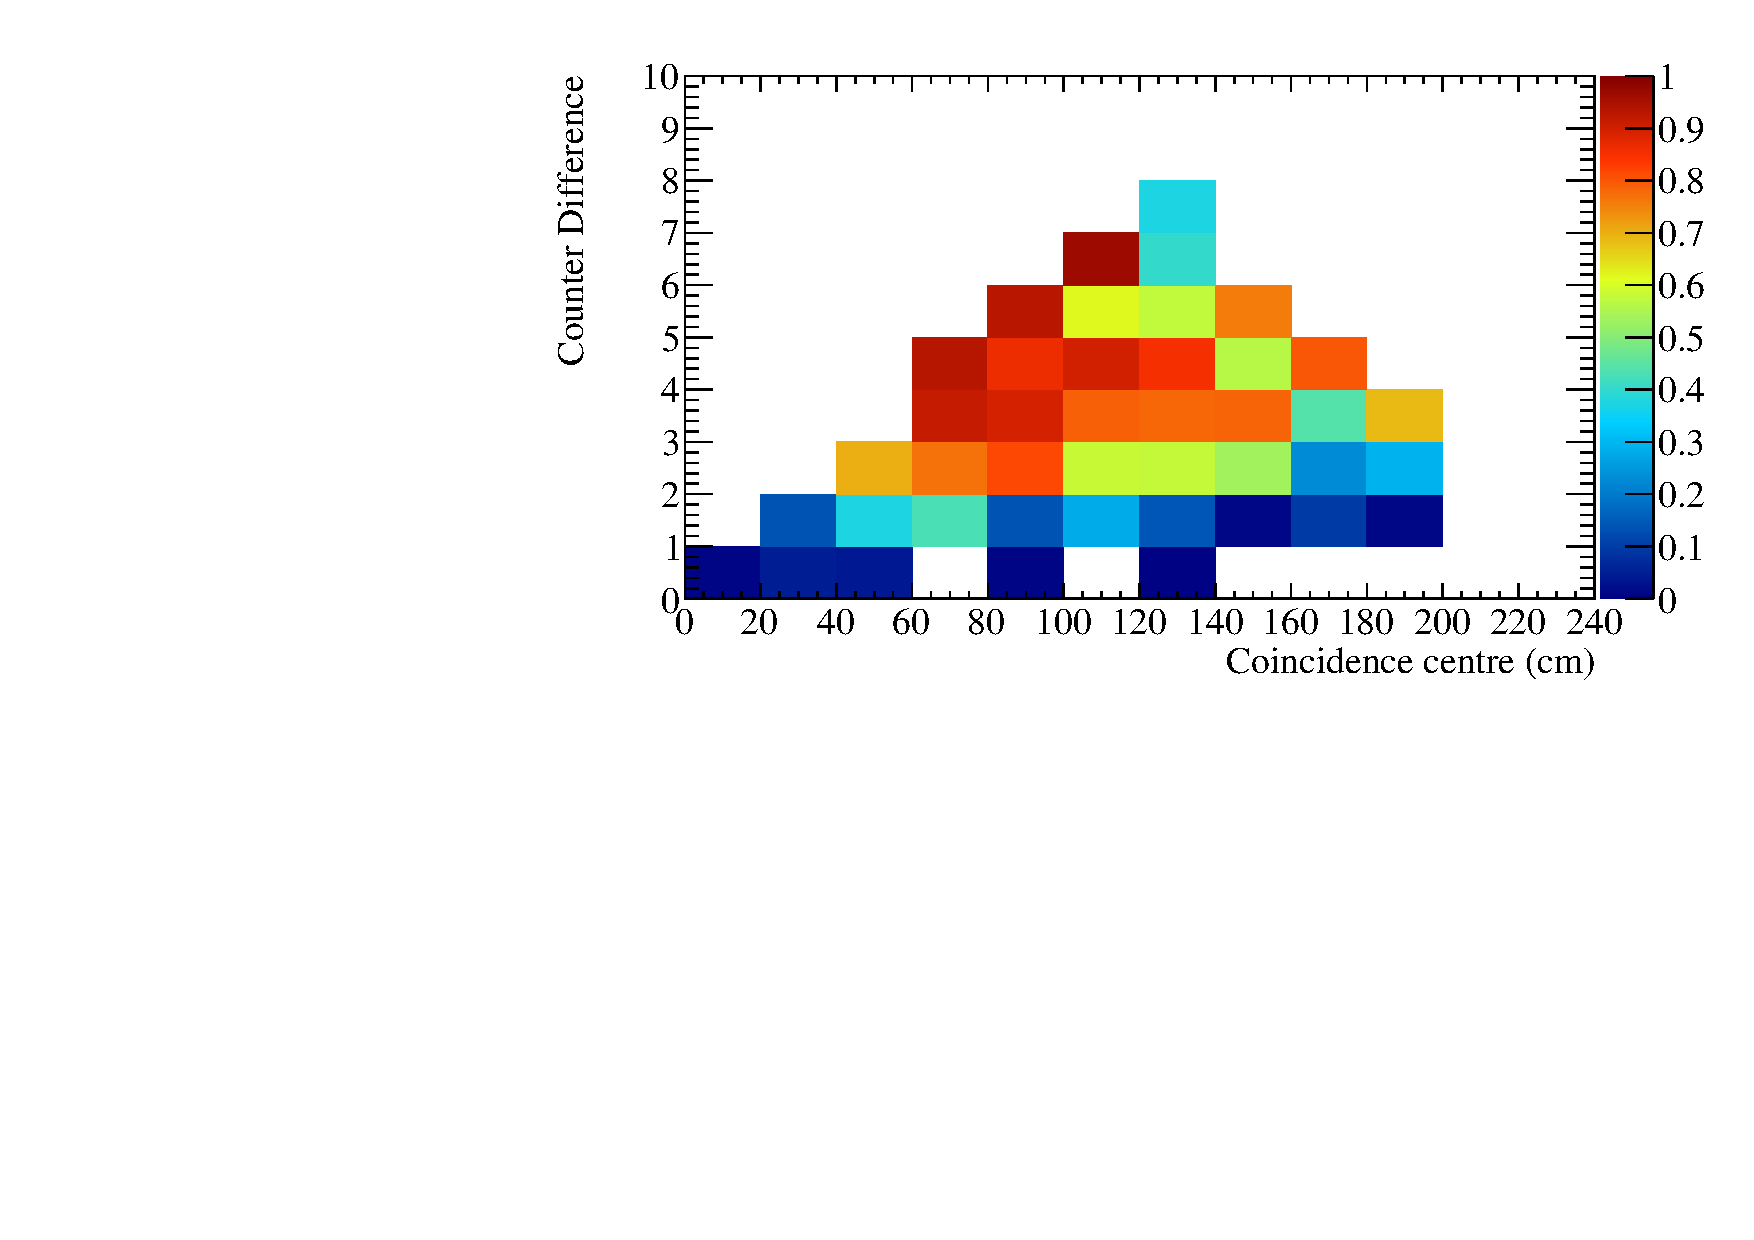
\includegraphics[width=\textwidth]{TwoDimensional_50cm}
    \caption{The difference in efficiencies at increasing distance from the APAs against increasing track angles relative to the APAs.}
    \label{fig:TwoDimCanvas}
  \end{subfigure}
  \hspace{0.08\textwidth}
  \begin{subfigure}{0.45\textwidth}
    \centering
    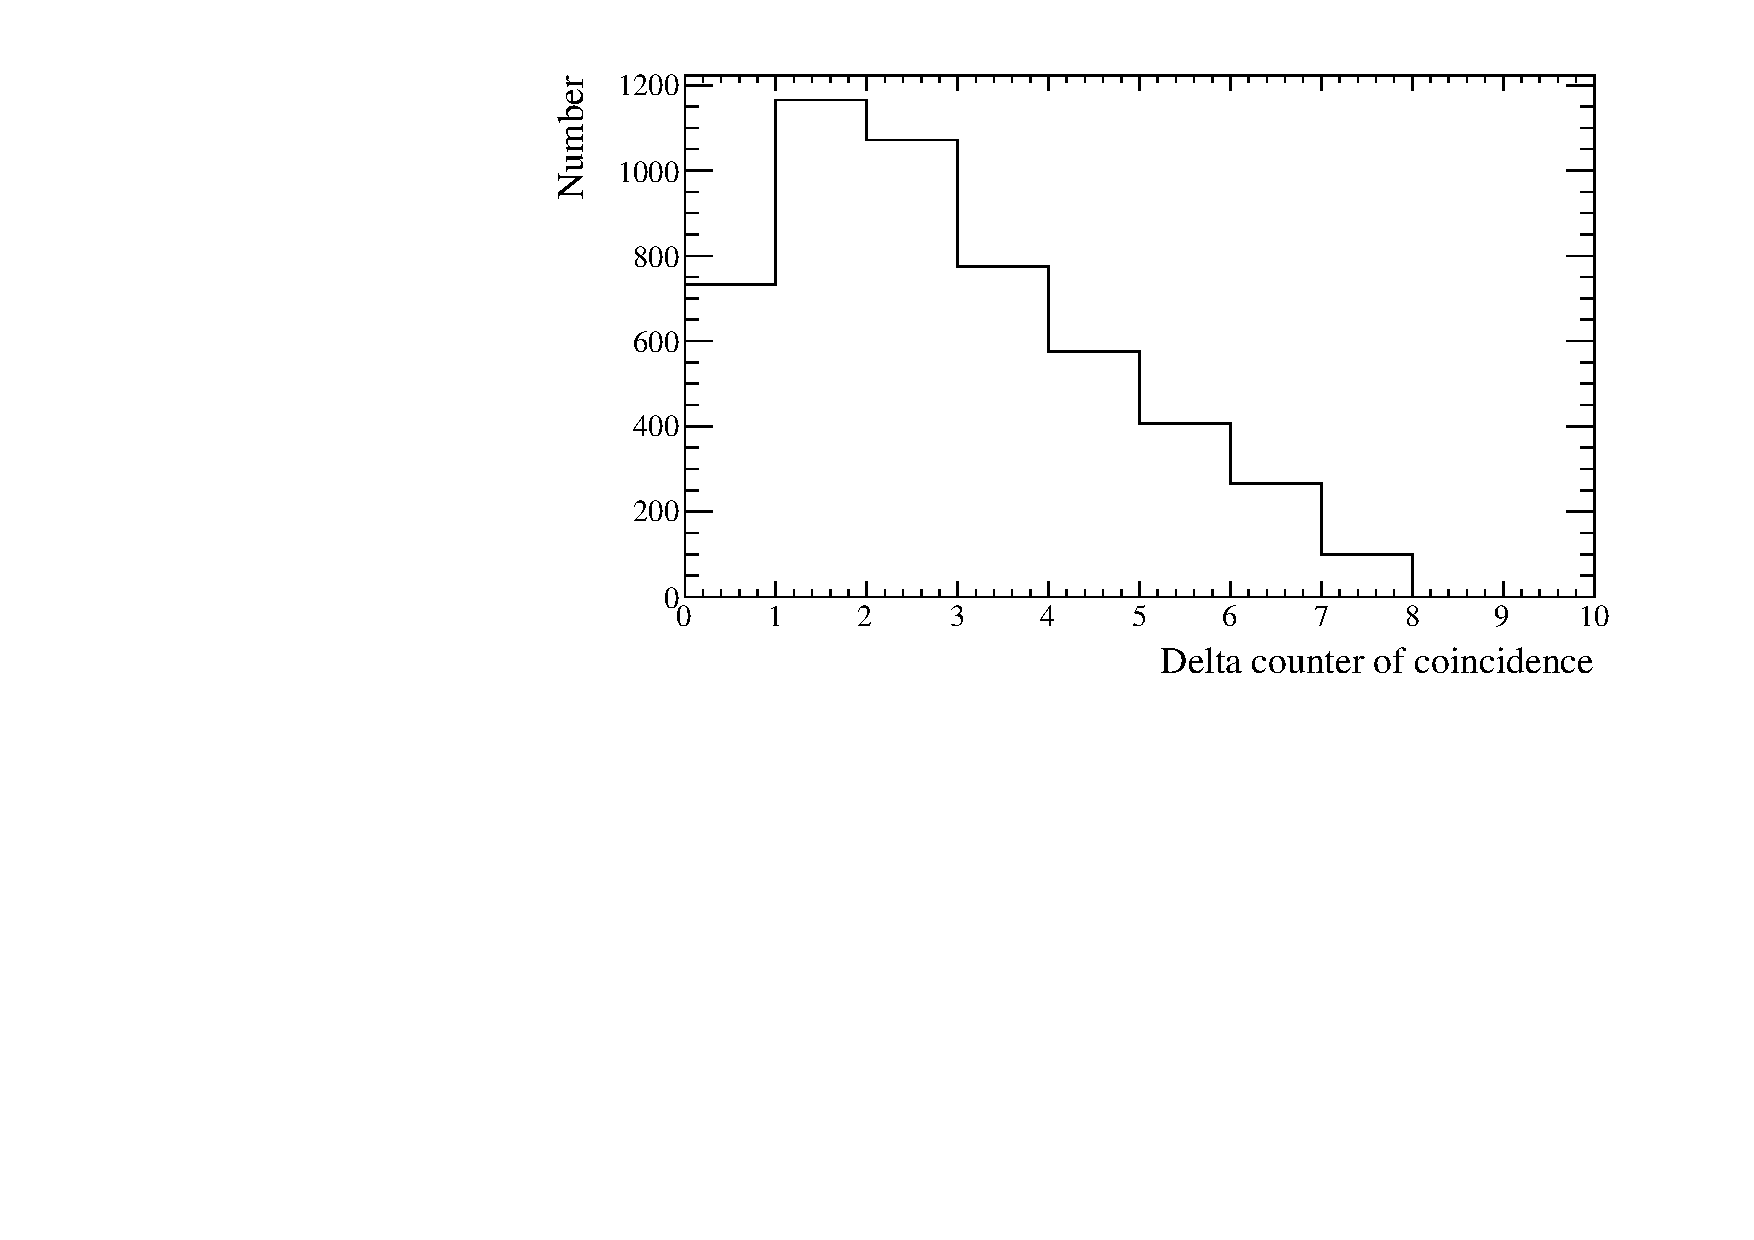
\includegraphics[width=\textwidth]{CounterDiffCan}
    \caption{The number of coincidences for each track angle.}
    \label{fig:CounterDiffFreq}
  \end{subfigure}
  \caption[Reconstruction efficiencies of through going tracks in the 35 ton data]{The reconstruction efficiencies for tracks which trigger an East-West coincidence in the 35 ton data and the number of events with each co-incidence over a 2 day running period.}
  \label{fig:DataRecoEffics}
\end{figure}
    
%********************************** % Fifth Section  *************************************
\section{Measuring interaction times using electron diffusion}  \label{DiffusionAnalysis}%Section - X.5
As electrons drift from the interaction point to the wire planes they become spread out in both time and space, this effect is known as diffusion and is an important property of electron transport in LAr which must be well understood. The mechanism by which diffusion occurs in LAr was first discussed by Atrazhev-Timoshkin~\citep{Atrazhev-Timoshkin}, and has since been developed to consist of a complete set of measurements for electric fields between 100 and 2000 V cm$^{-1}$~\citep{Li:2015rqa}. The diffusion of electrons is rarely isotropic and so the component that is transverse to the drift field and the component that is parallel to the drift field are normally measured separately. Diffusion parallel to the drift field is called longitudinal diffusion and is generally smaller than the component of diffusion that is transverse to the drift field. Figure~\ref{fig:DomDiffSchem} shows how diffusion can smear the electrons collected on a set of wires when the electrons are initially highly correlated in time and space. \\

\begin{figure}[h!]
  \centering
  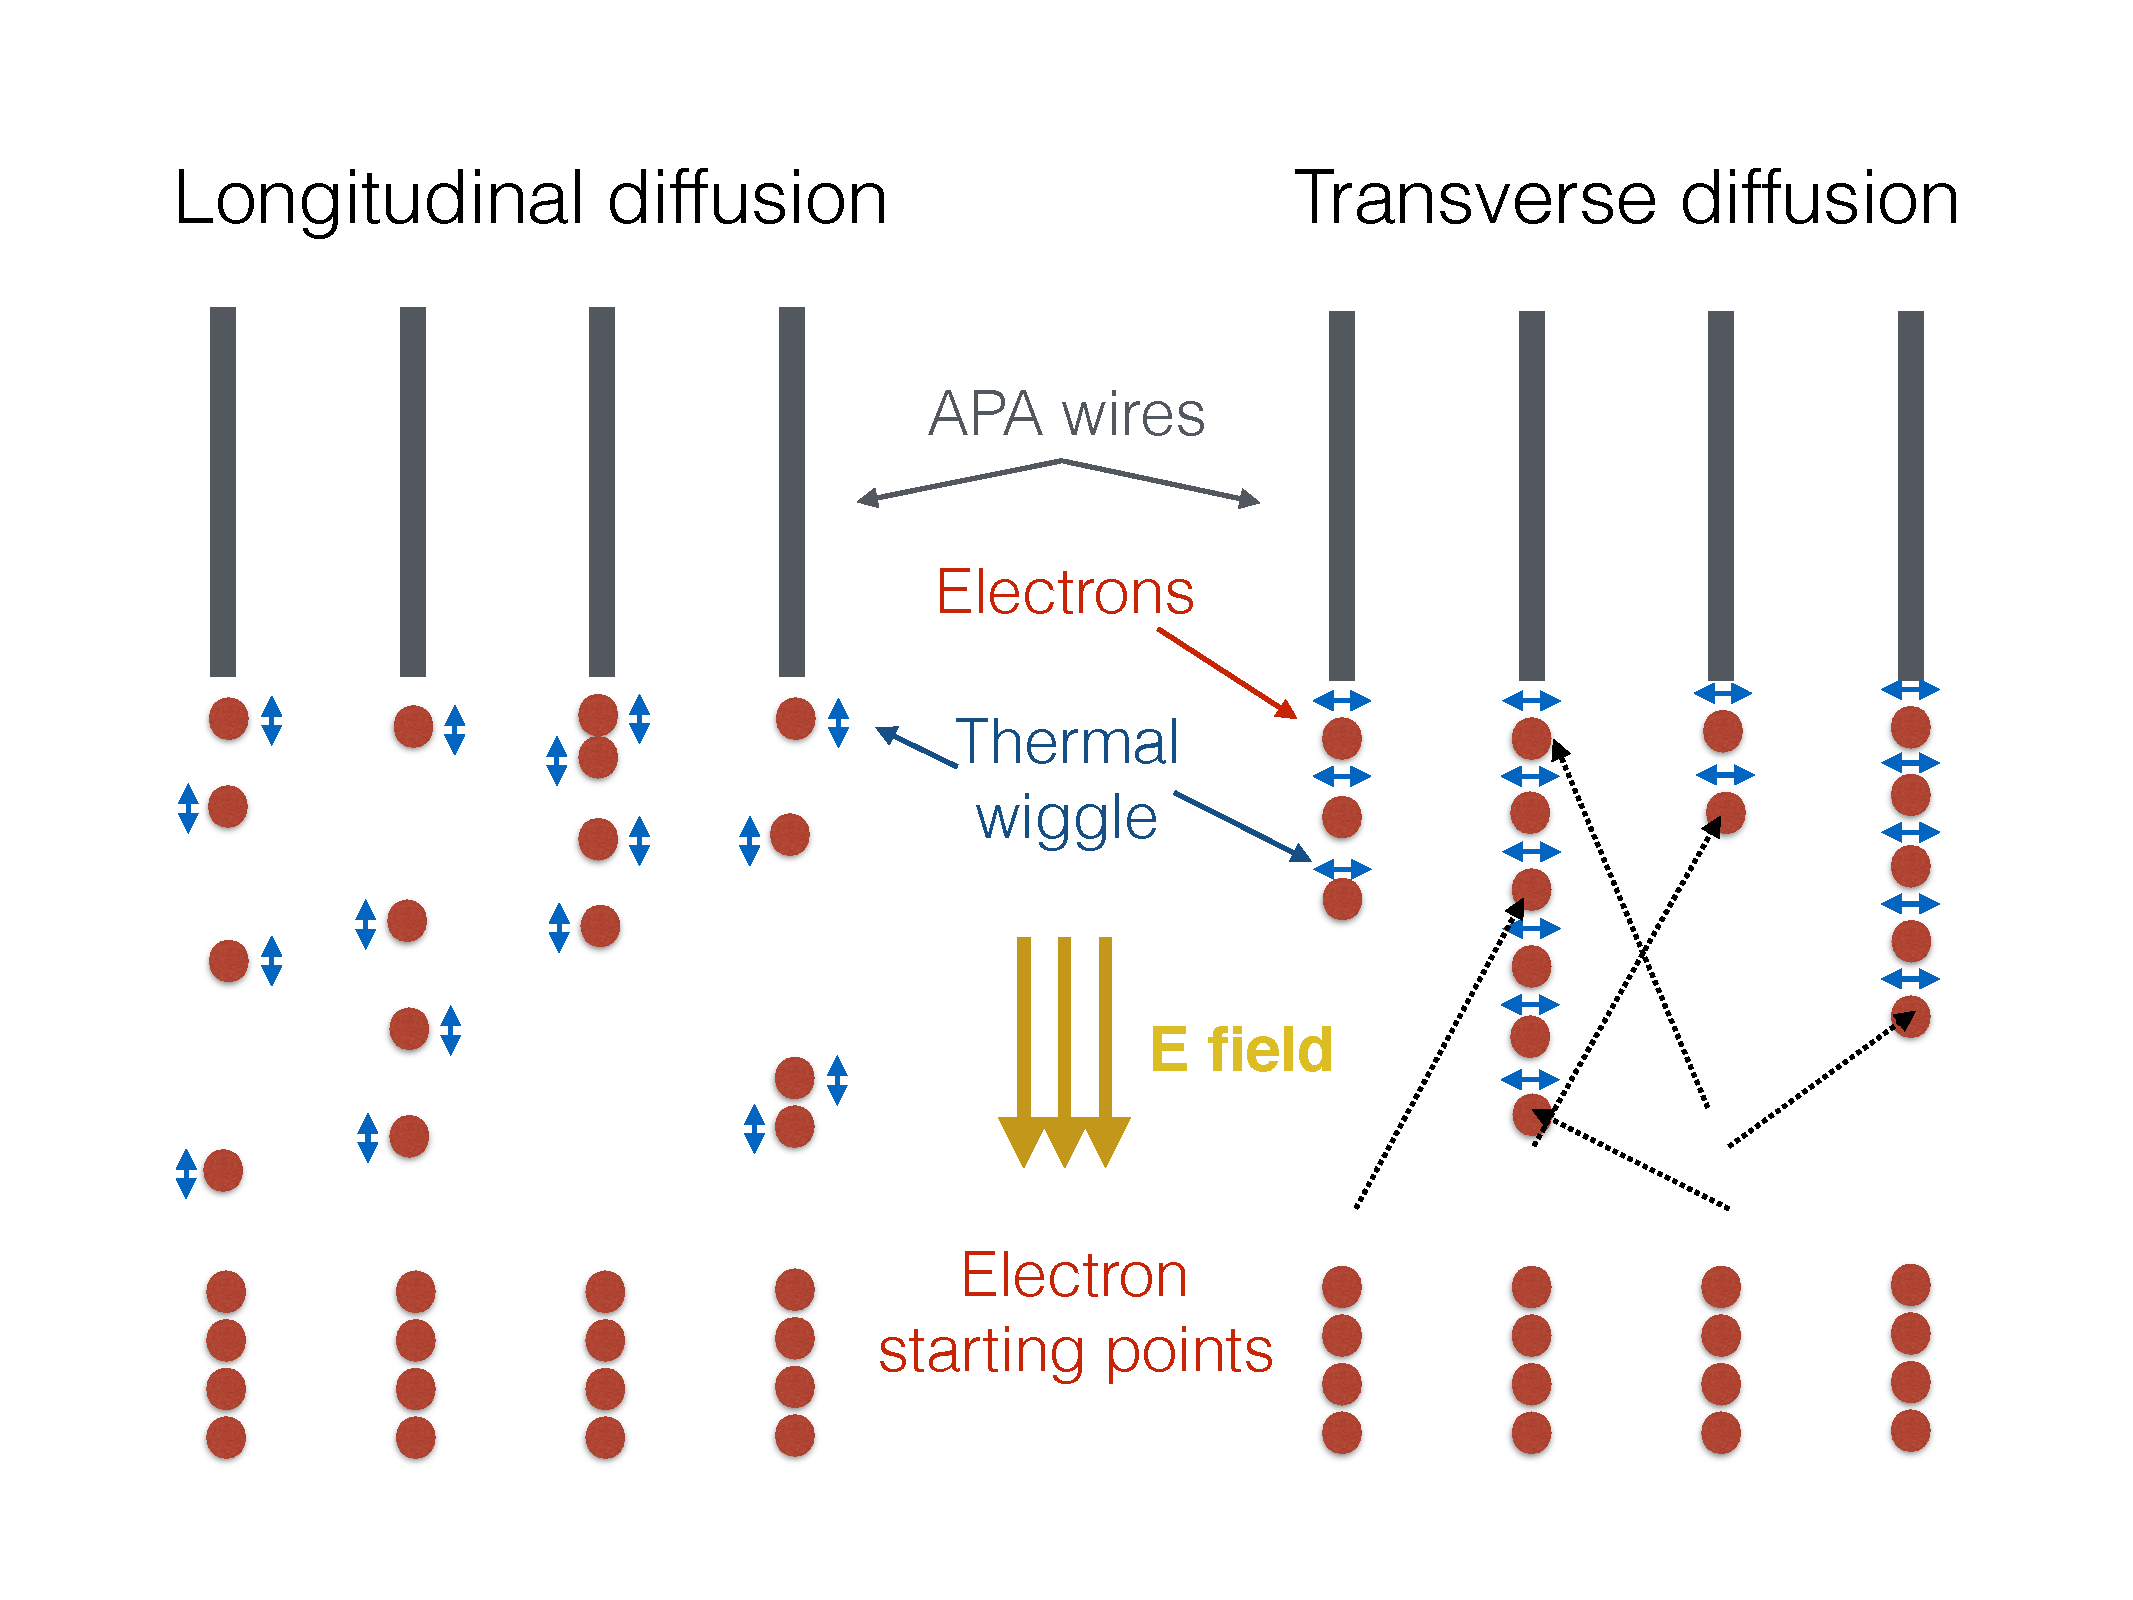
\includegraphics[width=0.85\textwidth]{DiffusionSchematic}
  \caption[Schematic showing the process of diffusion]{A schematic showing the difference between longitudinal diffusion (left) and transverse diffusion (right). In both cases four electrons are initially shown below four wires, a thermal wiggle is then applied in the drift direction and perpendicular to the drift direction in the longitudinal and transverse cases respectively. It can be seen that the effect of the thermal wiggles is to make the electrons spread out in time in the case of longitudinal diffusion and to spread out in space in the case of transverse diffusion~\citep{DomSeptMeeting}.}
  \label{fig:DomDiffSchem}
\end{figure}

Longitudinal diffusion has the effect of spreading the drifting electrons out in time causing signals to become wider in time and smaller in height as the total charge is conserved. The increasing hit width can be measured for increasing drift times (distances) provided the hits do not fall below a hit finding threshold. Transverse diffusion causes drifting electrons to spread out in space, changing the amount of charge deposited on a wire and reducing the charge resolution of the detector. Transverse diffusion is measured by discerning how the width of the hit charge distribution changes for increasing drift distances~\citep{DomSeptMeeting}. \\

Through-going particles make ideal tracks to study diffusion as they are minimally ionising and so have roughly constant energy depositions along their tracks. The tracks they produce can also cover a wide range of drift distances if they are not parallel to the APAs. The drift distances of hits within a track can be determined by matching the track with a counter coincidence as discussed at the end of Section~\ref{sec:DataAlgs} and then correcting the $x$ co-ordinates of the hits using the result of Equation~\ref{eq:HitTime_Int} in Equation~\ref{eq:HitTime}. \\

Traditionally the only way to determine an interaction time for a track is to match it to either an external calibration source such as whether it aligns with an external counter coincidence, or to match it to a flash of scintillation light as in Section~\ref{sec:SimInteractionTimes}. These techniques are particularly crucial for neutrino detectors on the Earths surface such as MicroBooNE where each neutrino interaction has a background of many cosmic muons which need to be disentangled in order correctly assign a scintillation flash to a reconstructed track. An example of an event which has many scintillation flashes and cosmic muons which need to be correctly associated is shown in Figure~\ref{fig:DiffLotsOfFlashes}. !!!I MAY HAVE A FIGURE FROM A PREVIOUS SECTION!!! However it may be possible that the change in hit width due to diffusion as a particle travels through the detector could be used to determine the interaction time, though this has not been attempted before. To study whether this is possible the effects of diffusion would have to be measured for a sample of tracks with known interaction times and orientations. \\

\begin{figure}[h!]
  \centering
  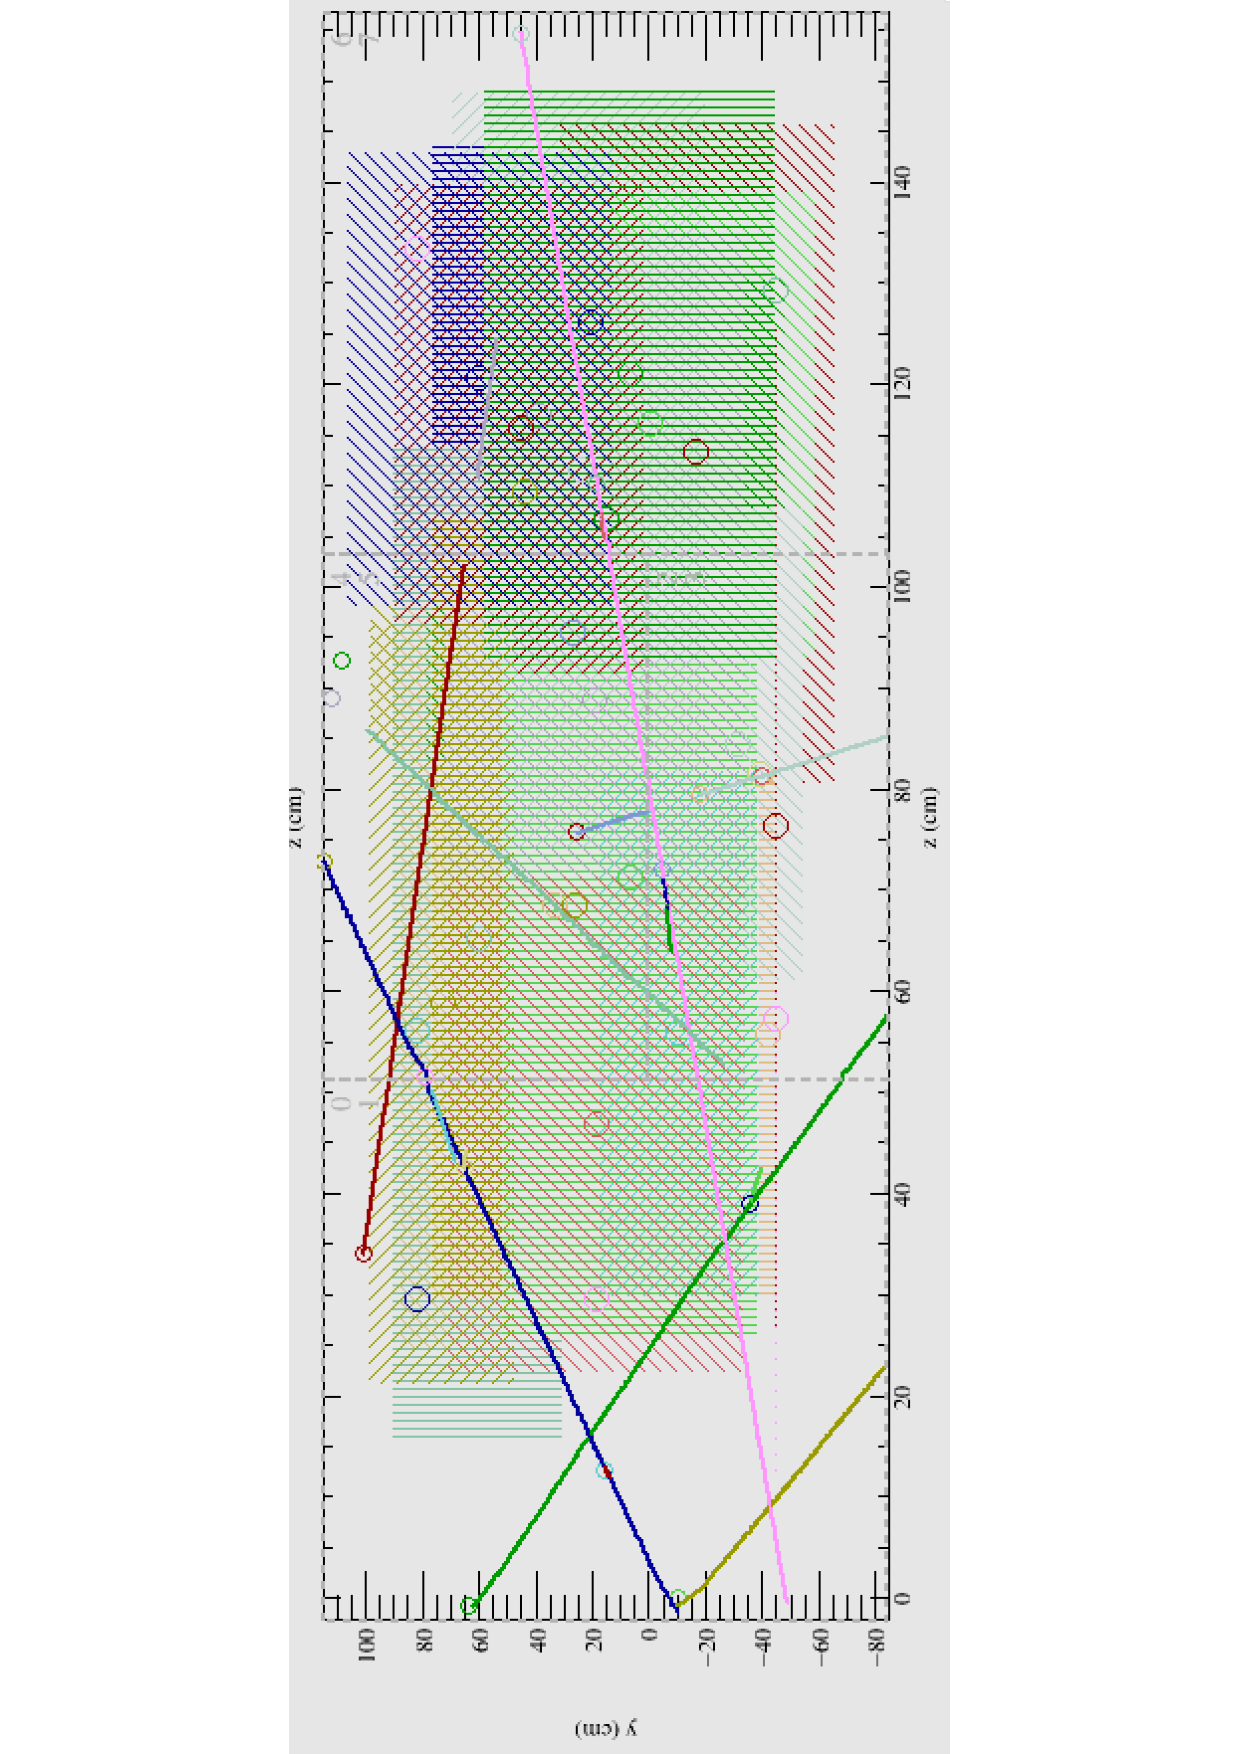
\includegraphics[width=0.85\textwidth]{LotsOfTrackFlash}
  \caption[A simulated event display showing multiple tracks and flashes in the 35 ton]
          {A simulated event display showing multiple tracks and flashes to be assigned to each other in the 35 ton. The coloured lines represent reconstructed tracks, whilst the coloured dashed boxes represent flashes.}
          \label{fig:DiffLotsOfFlashes}
\end{figure}

The 35 ton dataset is ideal for testing this hypothesis as the counters are able to provide a sample of tracks with known angles and interaction times which can be used to tune interaction time determination metrics. These metrics can then be applied to another sample of tracks where the interaction time is known but not used so that the accuracy of the calculated interaction times can be found. As longitudinal diffusion is the dominant effect that increases the hit width transverse diffusion will not be directly considered further. However, as noted in Section~\ref{sec:DataAlgs} the noise level in the 35 ton data causes reconstruction issues and so a baseline measurement on an ideal detector is also useful, Monte Carlo can provide this sample. \\

%********************************** % Fifth.First Section  *************************************
\subsection{Determining interaction times in 35 ton data}
When calculating the determination metrics only hits on wires which are not noisy want to be considered. This is because wires with a high level of correlated noise observe hits with a wider RMS as shown by Figure~\ref{fig:DomsHitModel} where when a baseline noise of 10 ADC counts was added to a simulated hit with a peak value of 50 ADC counts and RMS 10 ticks the width was seen to increase by over 10\%. Hits with delta rays also need to be removed as the deposited energy will be larger and over a longer period of time than hits from the main track, this will make the RMS of the individual hit wider and also increase the width of the charge distribution for the track. In order to remove these hits only hits which satisfy the following cuts are used:
\begin{itemize}
\item No hit on the same wire within 50 ticks of the hit in question - removes delta rays.
\item No more than 10 hits on the same wire in the whole 15,000 tick data sample - removes clearly noisy wires.
\end{itemize}
These cuts will clearly become much more restrictive as the noise level in the detector increases, but they are essential in order to collect a dataset which is not overpowered by noise. A further restriction applied is that only collection plane hits are used as the charge resolution is better and the signals are unipolar as opposed to bipolar meaning that a Gaussian can be easily fitted to the signals. Additionally the $signal/noise$ ratio on the collection planes was much higher than on the induction planes for the 35 ton dataset and so the hits could be much more reliably reconstructed. \\

\begin{figure}[h!]
  \centering
  \begin{subfigure}{0.45\textwidth}
    \centering
    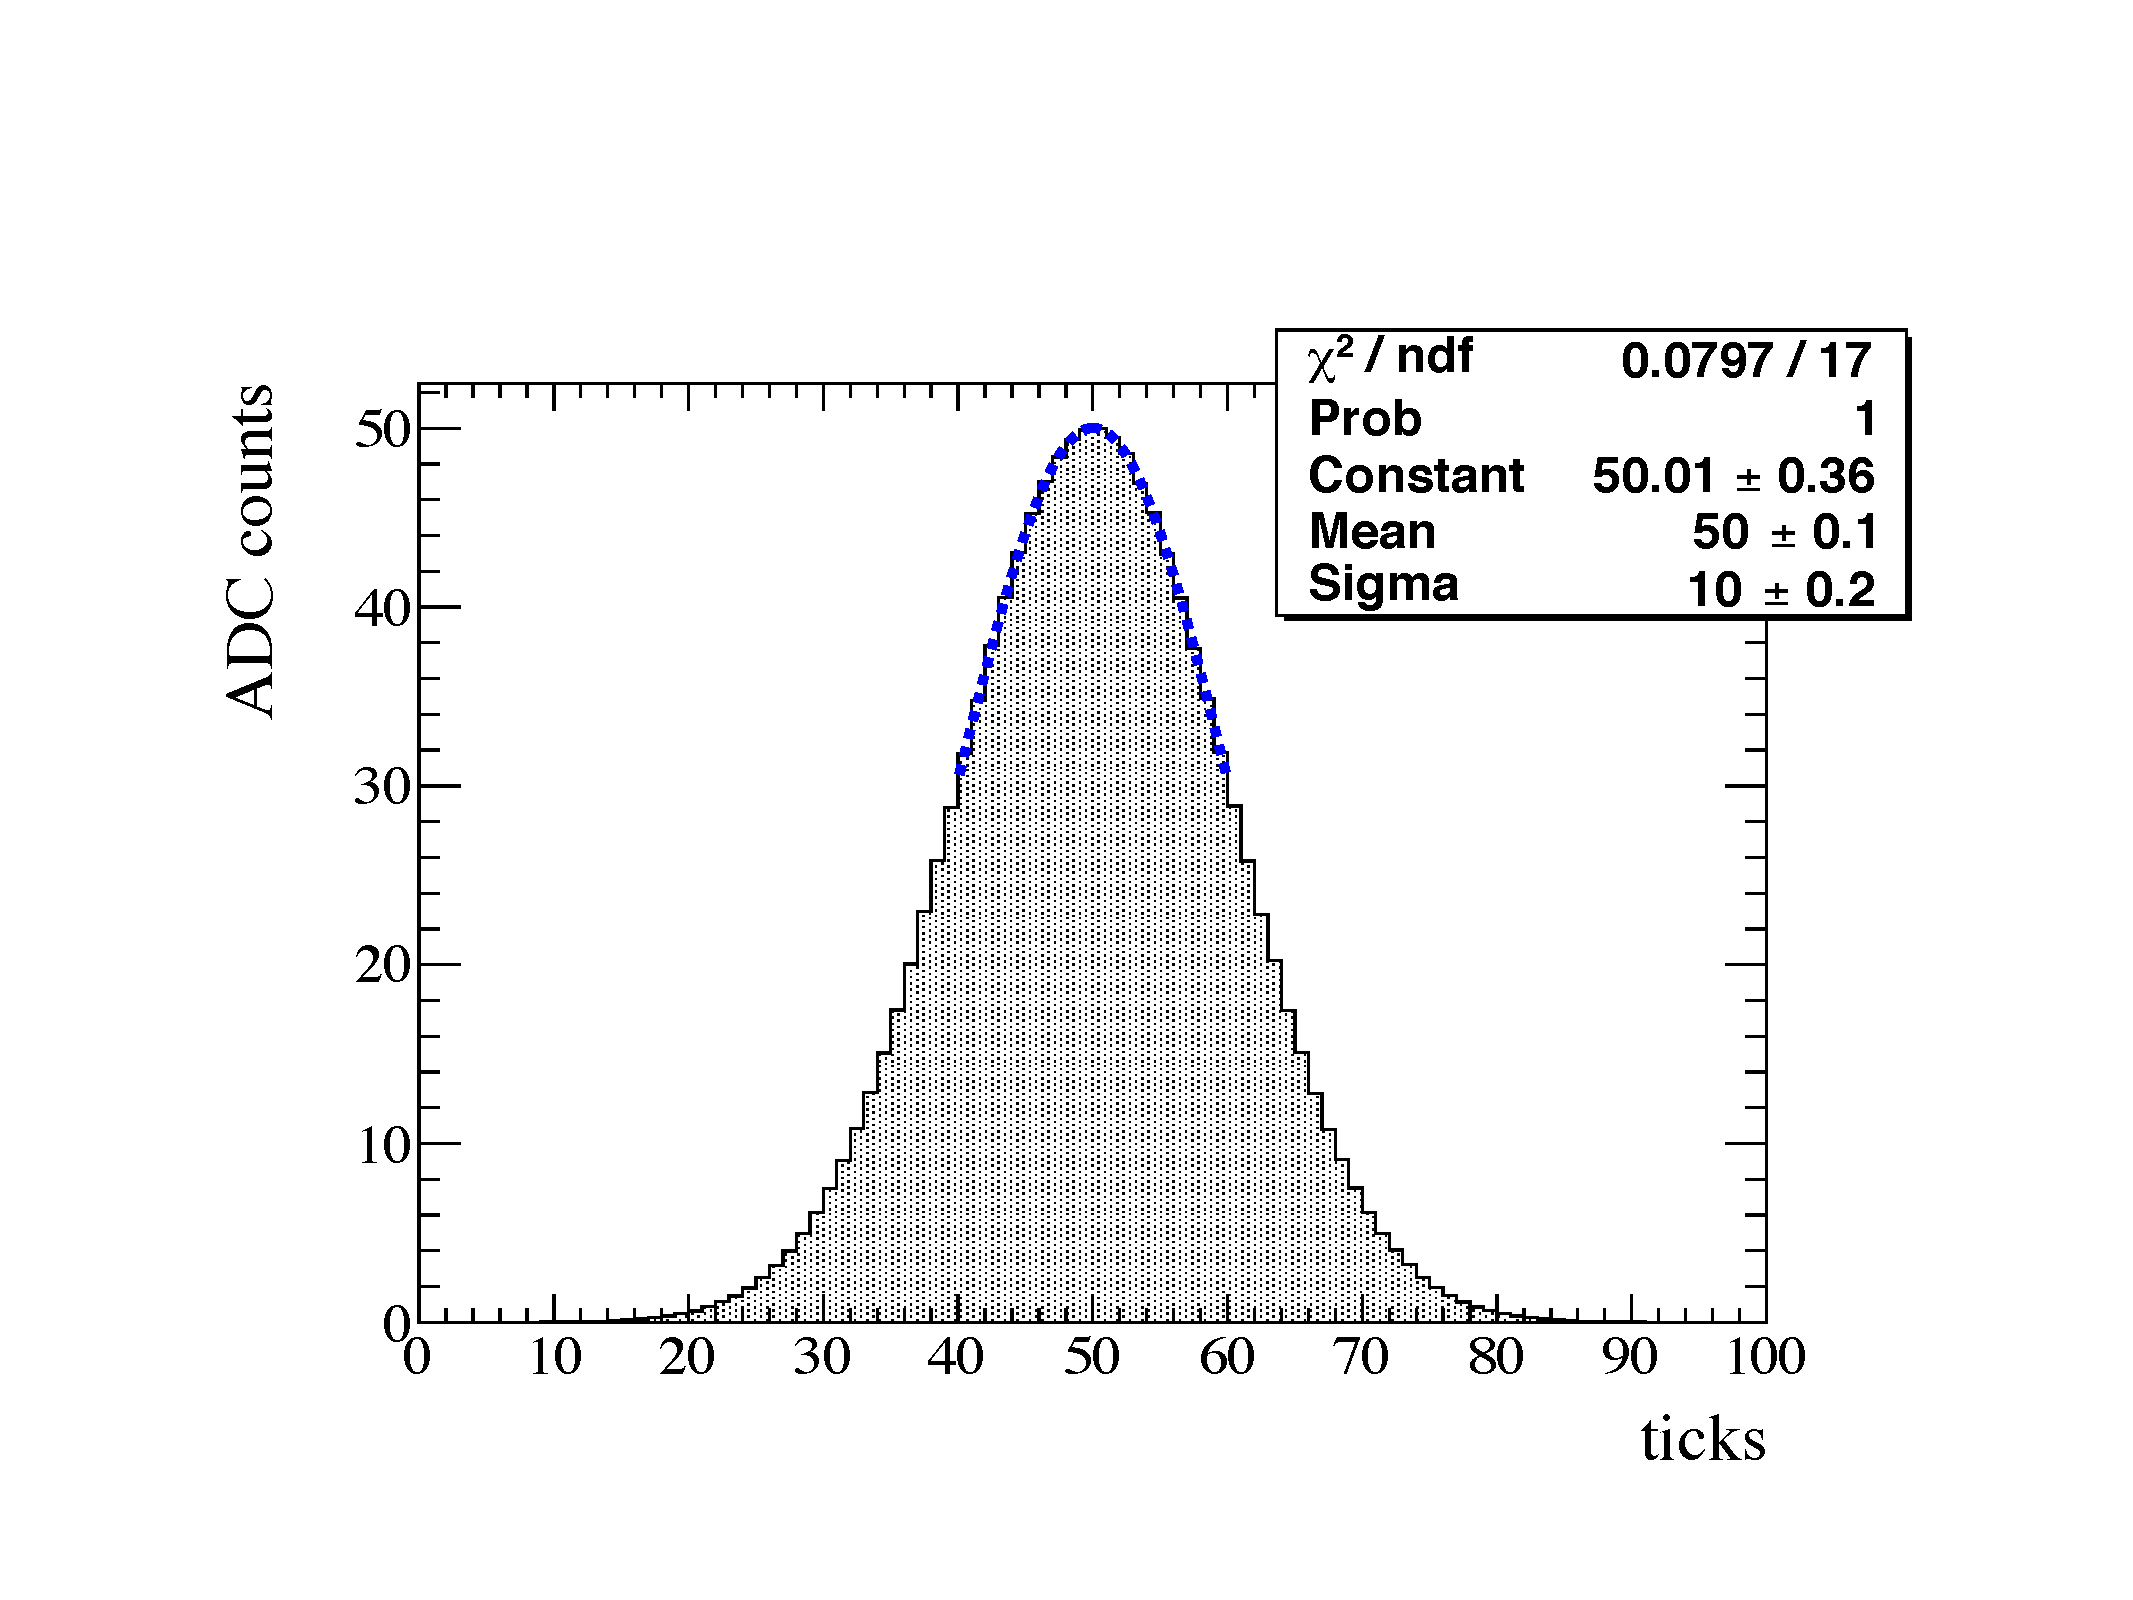
\includegraphics[width=\textwidth]{ToyGauss_Raw}
    \caption{A toy Gaussian hit with width 10 ticks, and amplitude 50 ADC counts.}
  \end{subfigure}
  \hspace{0.08\textwidth}
  \begin{subfigure}{0.45\textwidth}
    \centering
    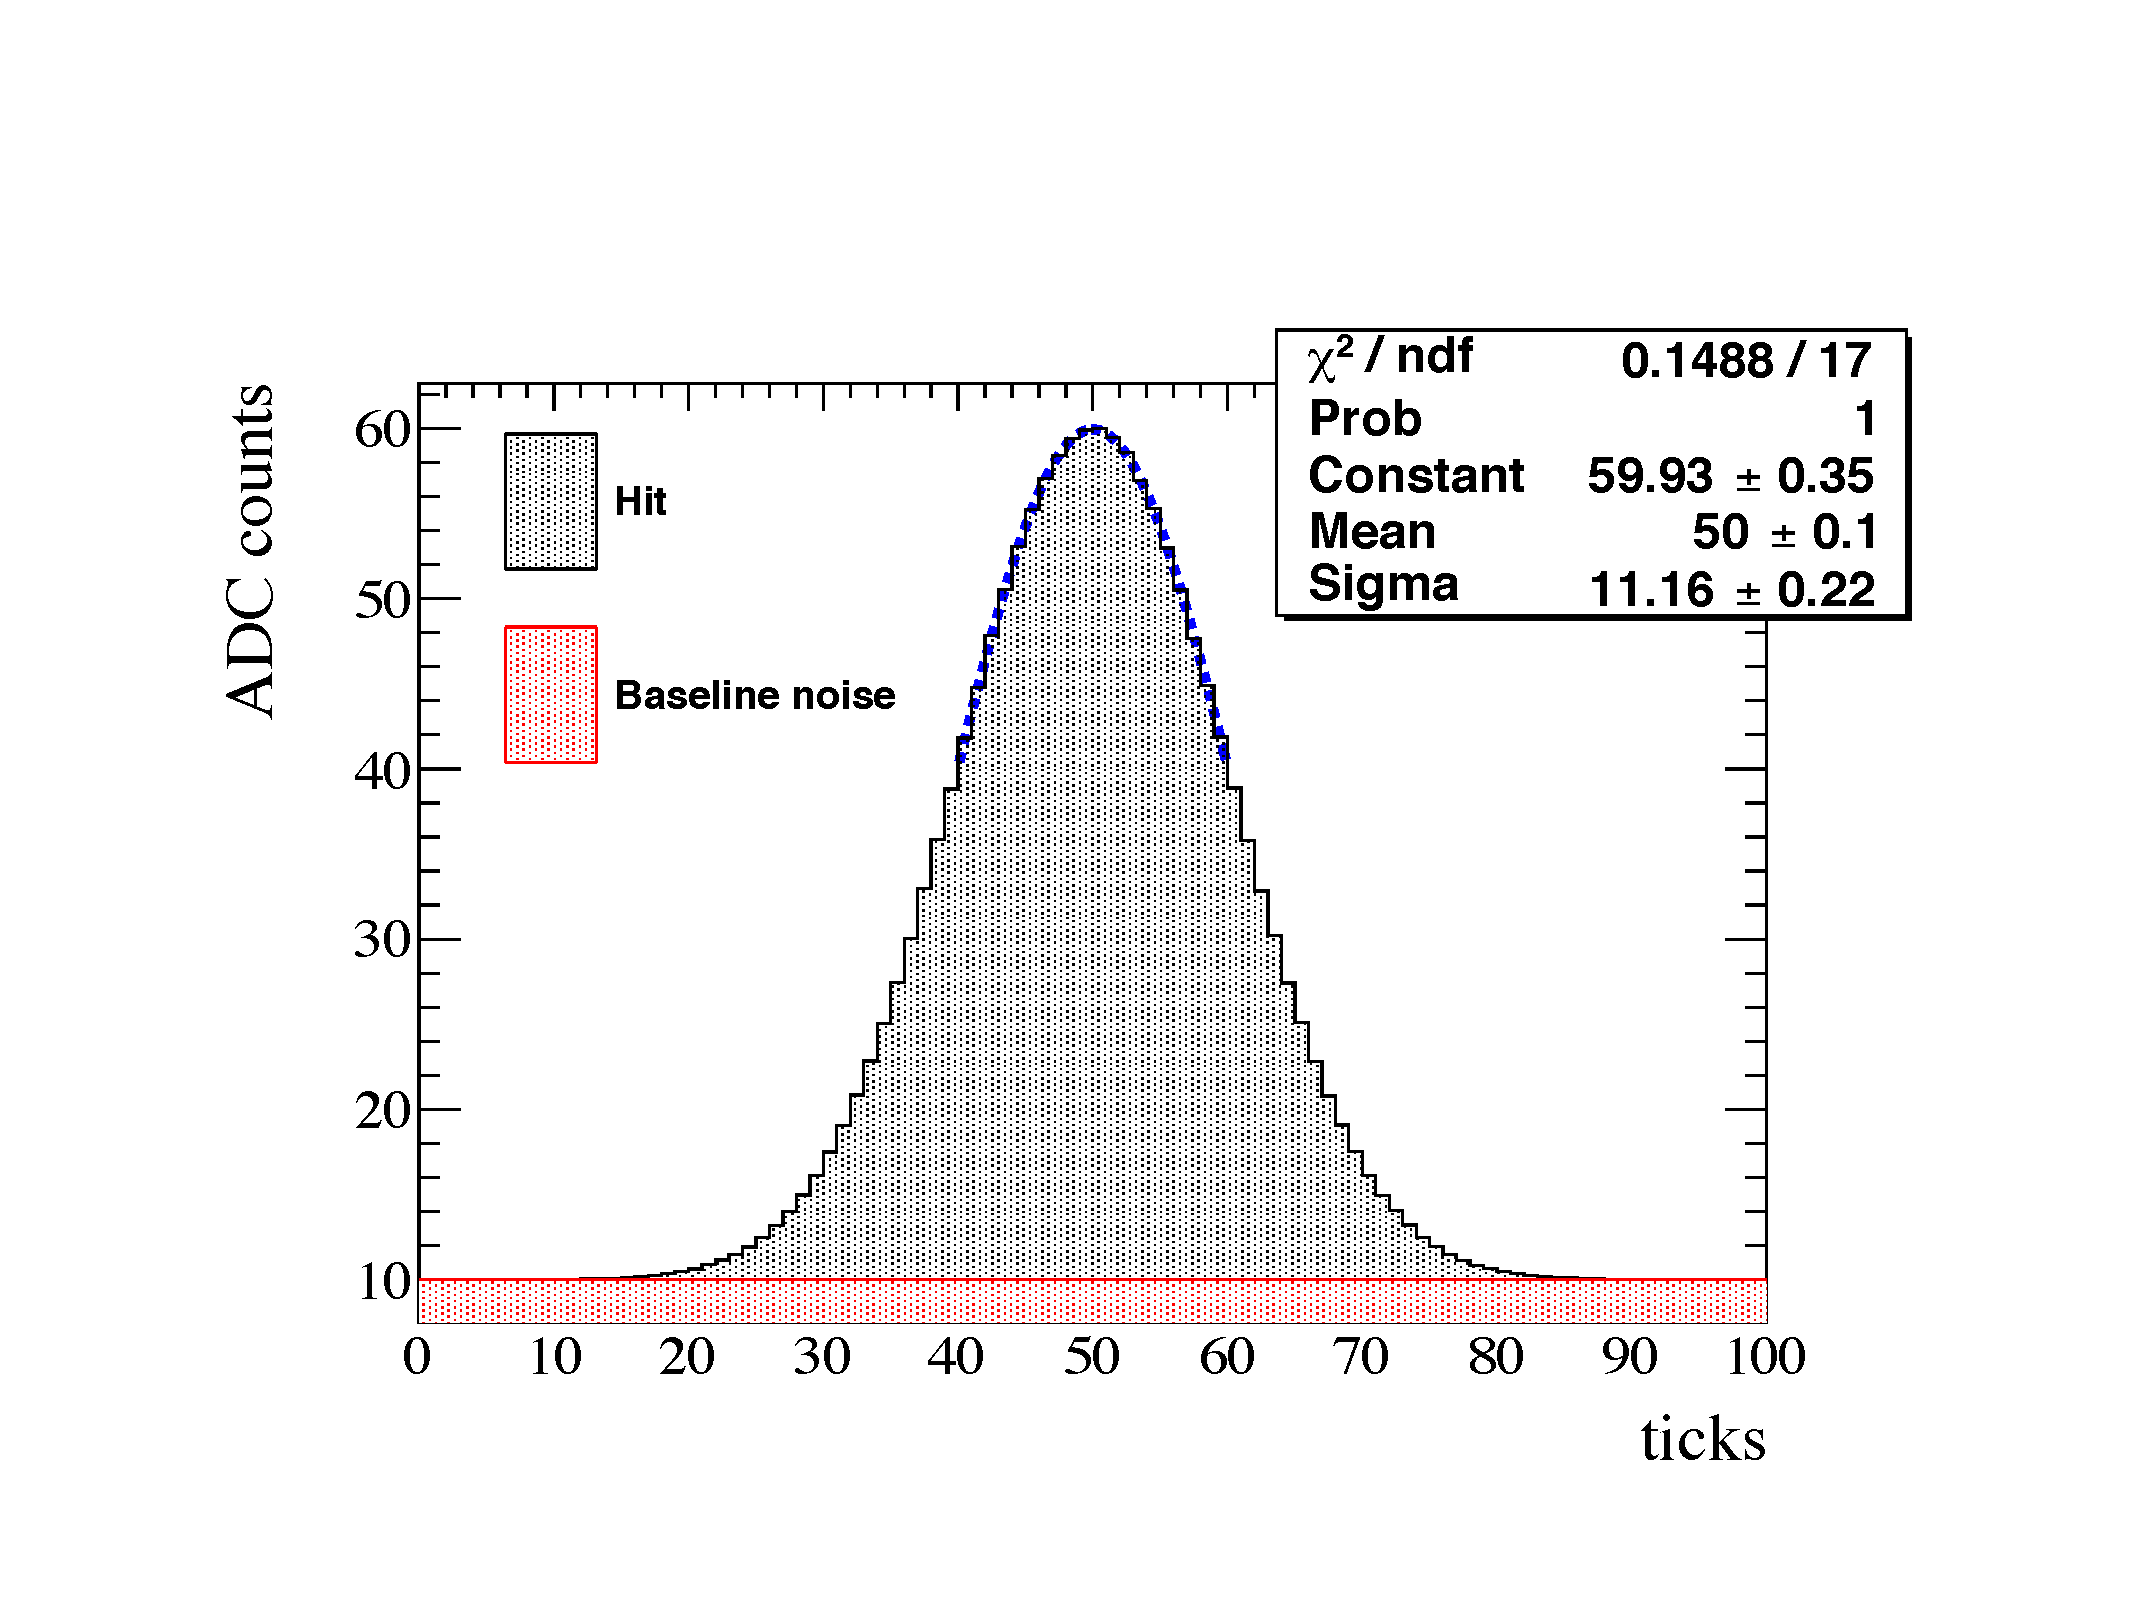
\includegraphics[width=\textwidth]{ToyGauss_Noise}
    \caption{The reconstructed width when a noise baseline of 10 ADC counts is added.}
  \end{subfigure}
  \caption[The effect of adding a noise baseline to a hit]
          {The width of a Gaussian fit is seen to increase by more than 10\% when a noise baseline is added to the signal showing that noise can cause the measured width of a hit to increase~\citep{DomSeptMeeting}.}
          \label{fig:DomsHitModel}
\end{figure}  

Diffusion is a track angle dependent property and so track angle ranges have to be considered independently. From Figure~\ref{fig:DataRecoEffics} it can be seen that tracks with a counter difference of 4 are the best reconstructed in data and so reference will be given to these tracks, though the same procedure is applied to all track angles. The tracks are considered en masse and so the hits for every track are separated into 10 cm regions of increasing drift distance from the APAs. The following quantities are calculated for each 10 cm drift region:
\begin{itemize}
\item The hit $RMS$ - the most direct way to measure transverse diffusion.
\item The hit $RMS/Charge$ - an attempt to incorporate the effect of impurities in the LAr for relatively low purity data which will have a drift distance dependence.
\end{itemize}
Fitting Gaussian's around the peaks of the distributions will yield the most probable values for the drift regions, as is shown in Figure~\ref{fig:DiffDataHitFit}. \\

\begin{figure}[h!]
  \centering
  \begin{subfigure}{0.45\textwidth}
    \centering
    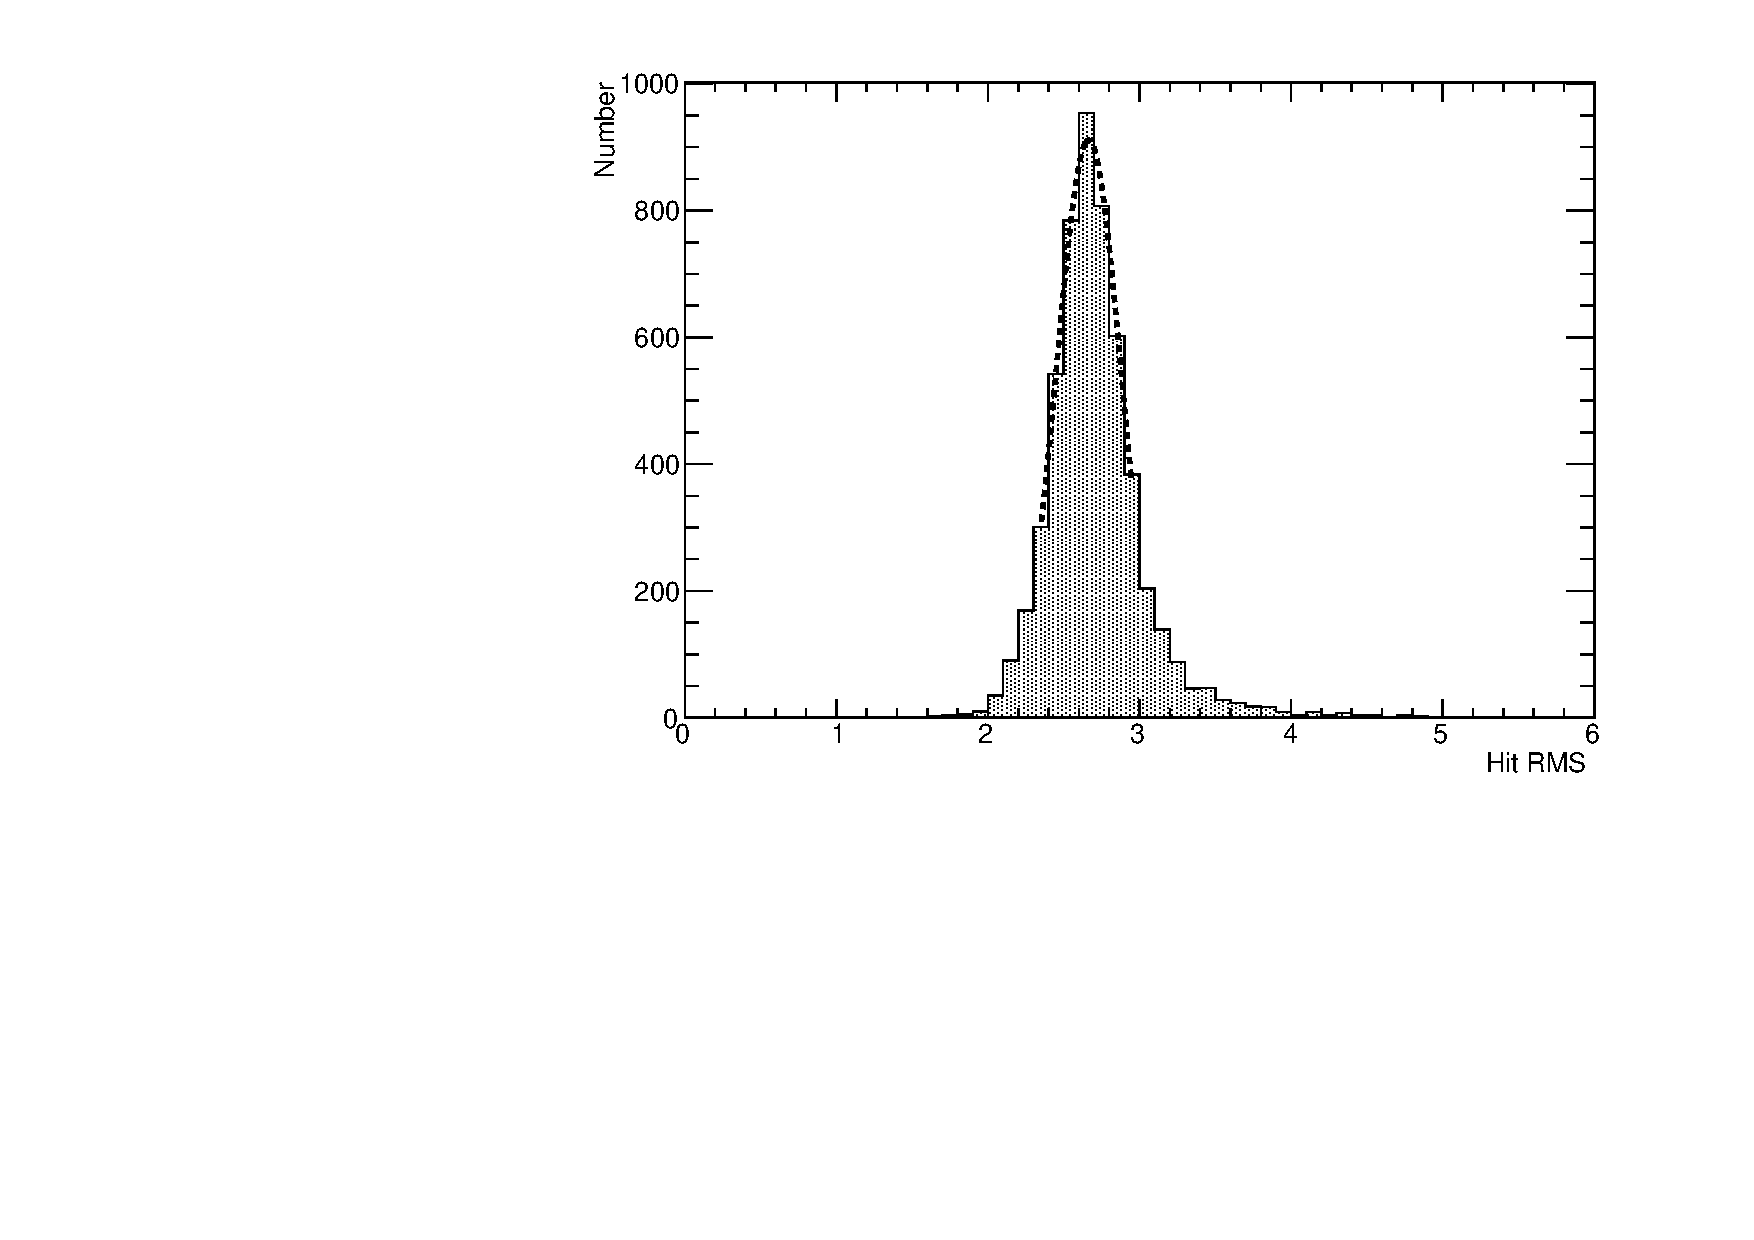
\includegraphics[width=\textwidth]{DataCan_0}
    \caption{The most probable hit $RMS$ value at $x =$ 20 cm for tracks with a counter difference of 4.}
  \end{subfigure}
  \hspace{0.08\textwidth}
  \begin{subfigure}{0.45\textwidth}
    \centering
    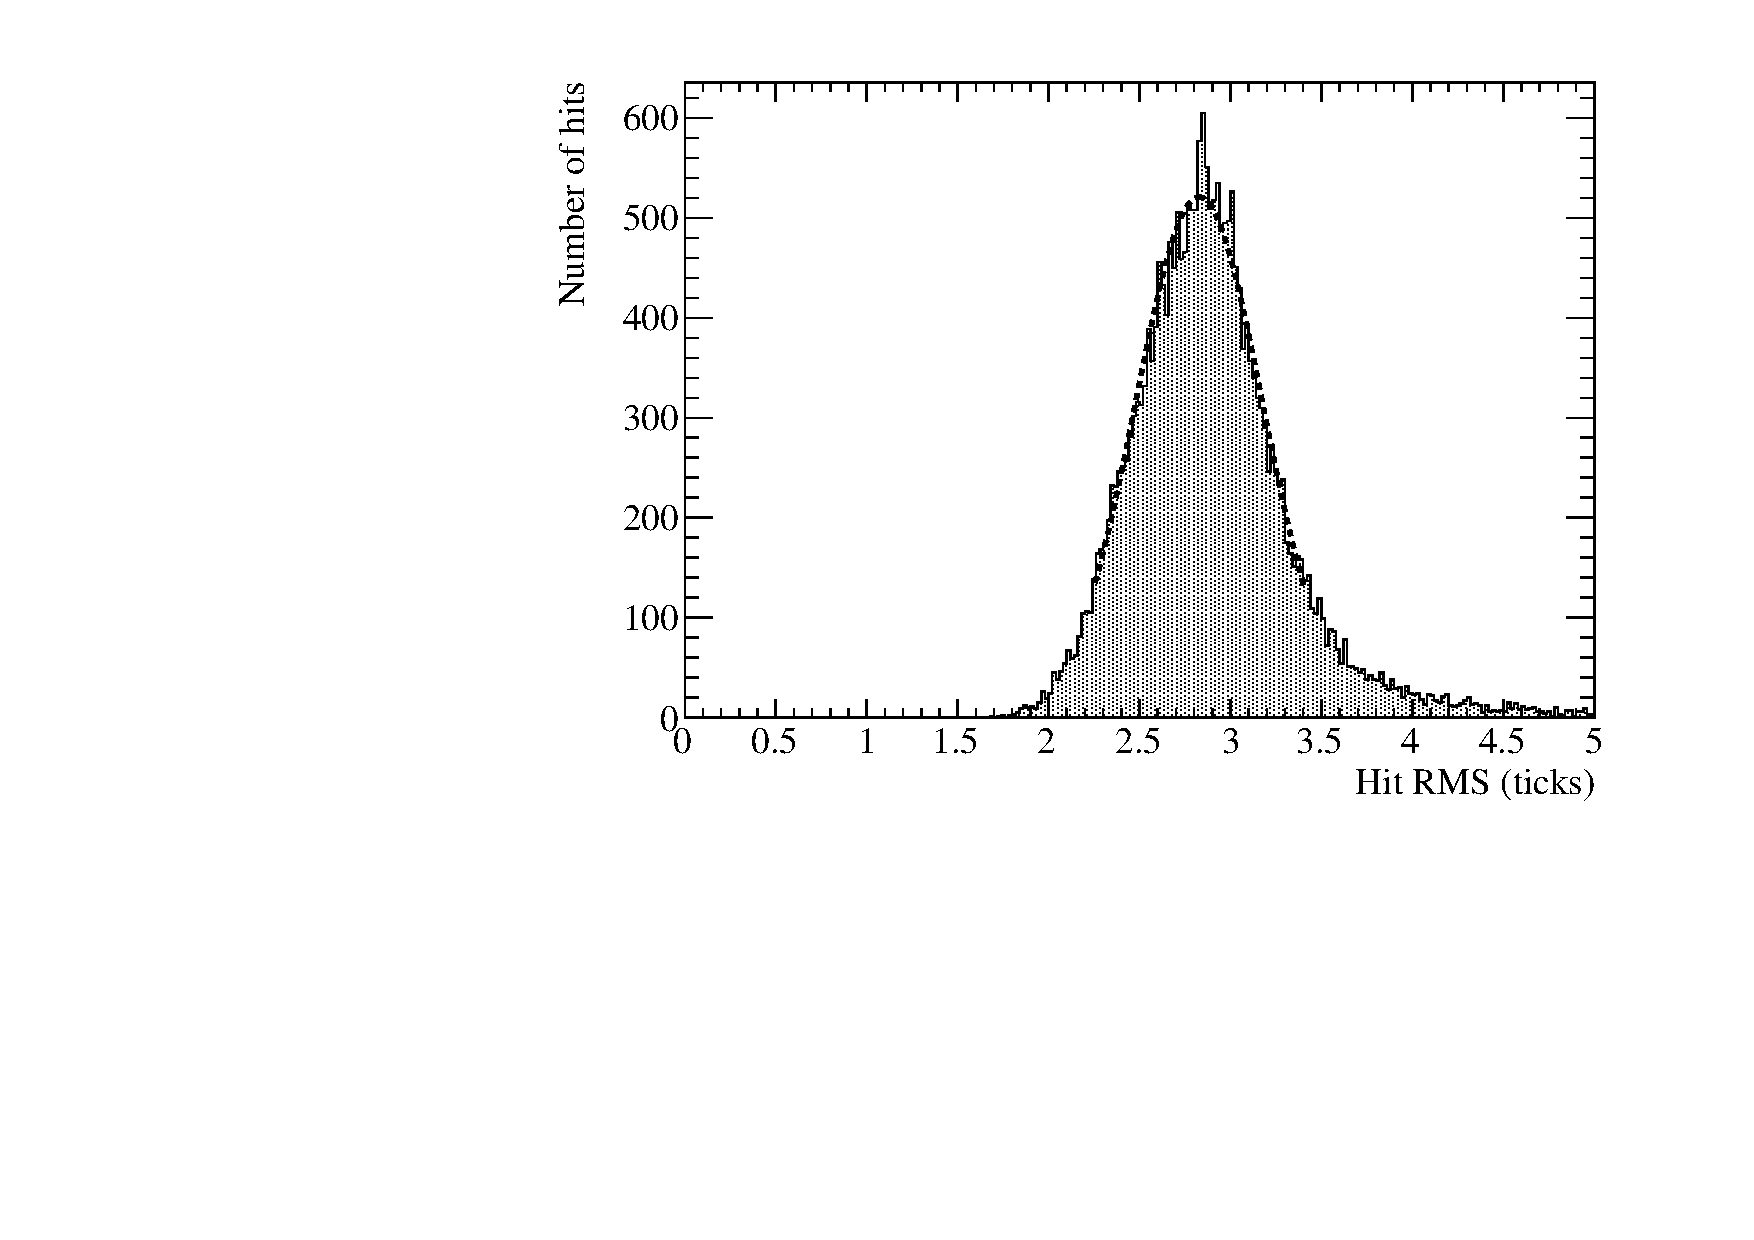
\includegraphics[width=\textwidth]{DataCan_1}
    \caption{The most probable hit $RMS$ value at $x =$ 140 cm for tracks with a counter difference of 4.}
  \end{subfigure}
  \begin{subfigure}{0.45\textwidth}
    \centering
    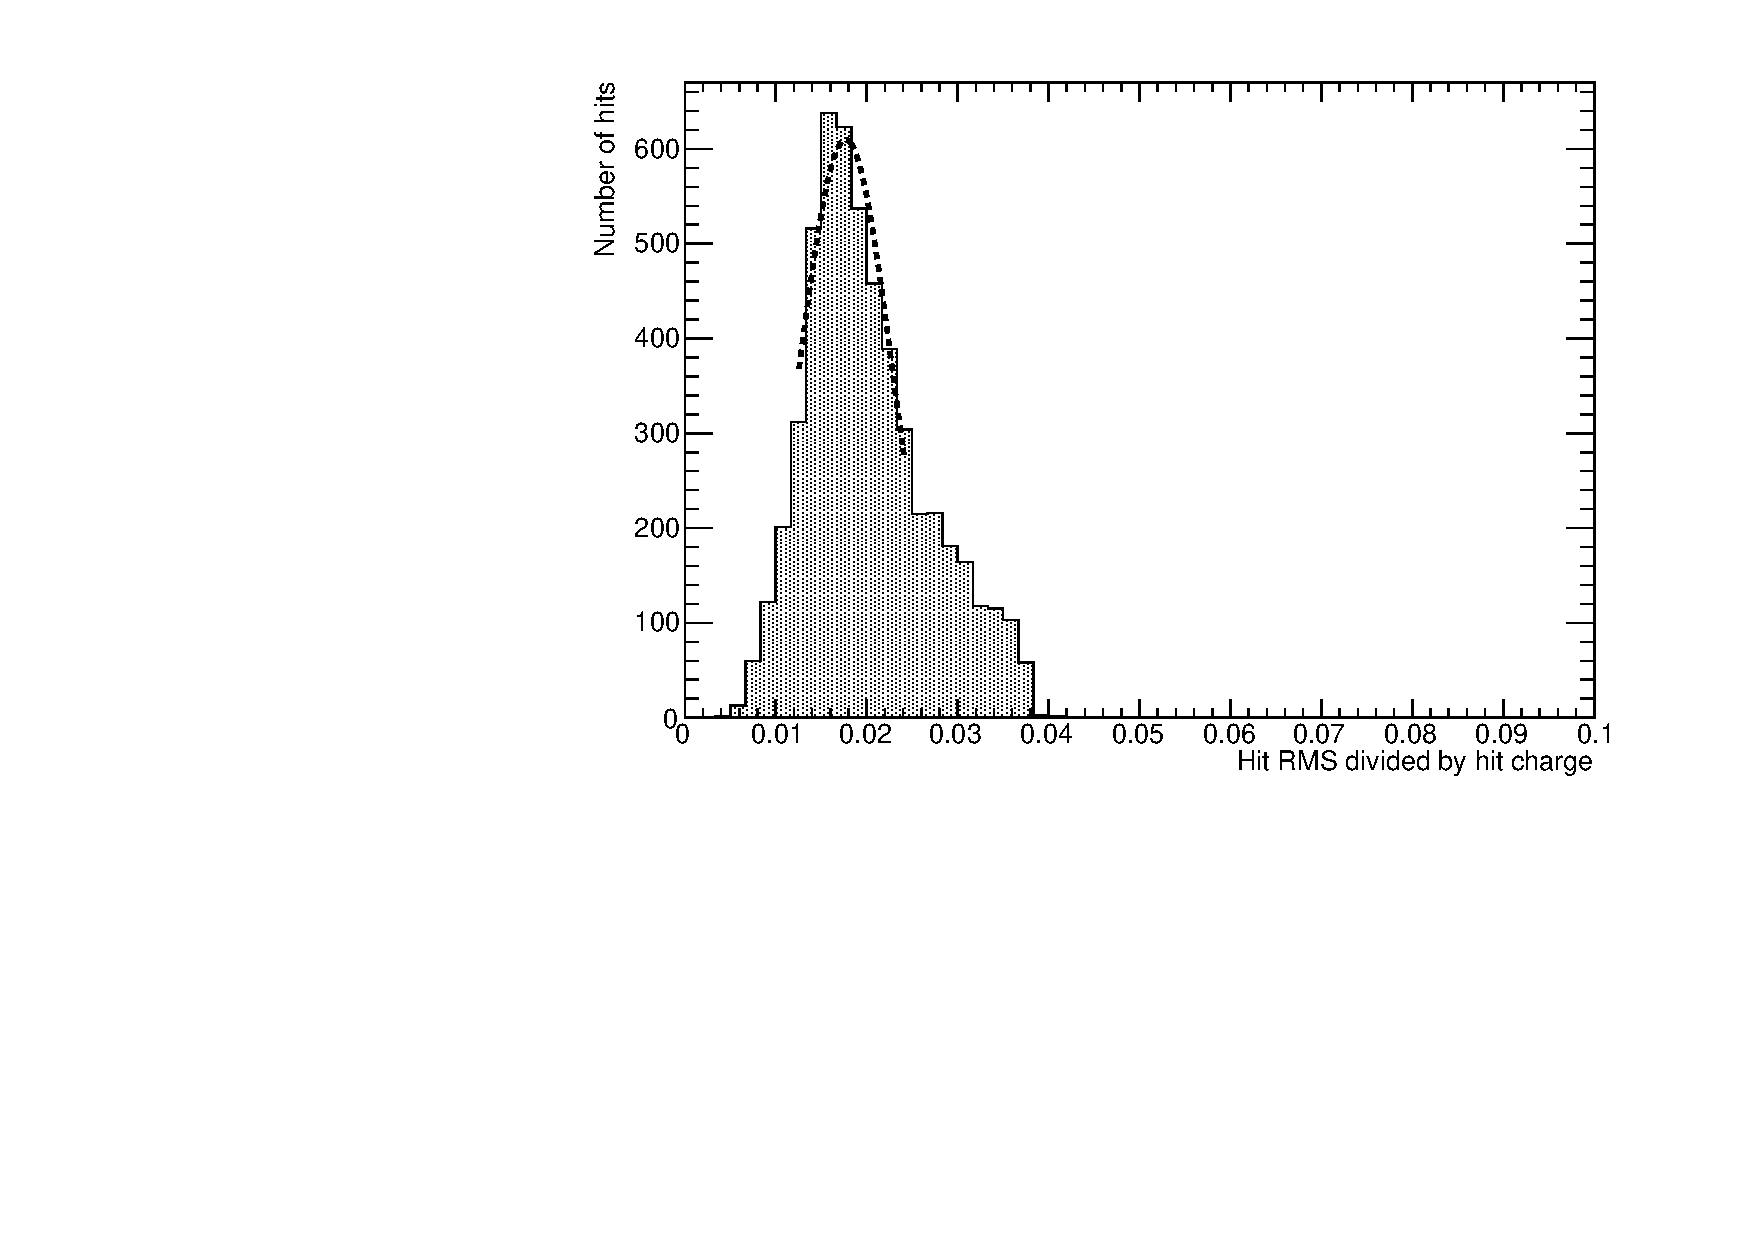
\includegraphics[width=\textwidth]{DataCan_2}
    \caption{The most probable hit $RMS/Charge$ value at $x =$ 20 cm for tracks with a counter difference of 4.}
  \end{subfigure}
  \hspace{0.08\textwidth}
  \begin{subfigure}{0.45\textwidth}
    \centering
    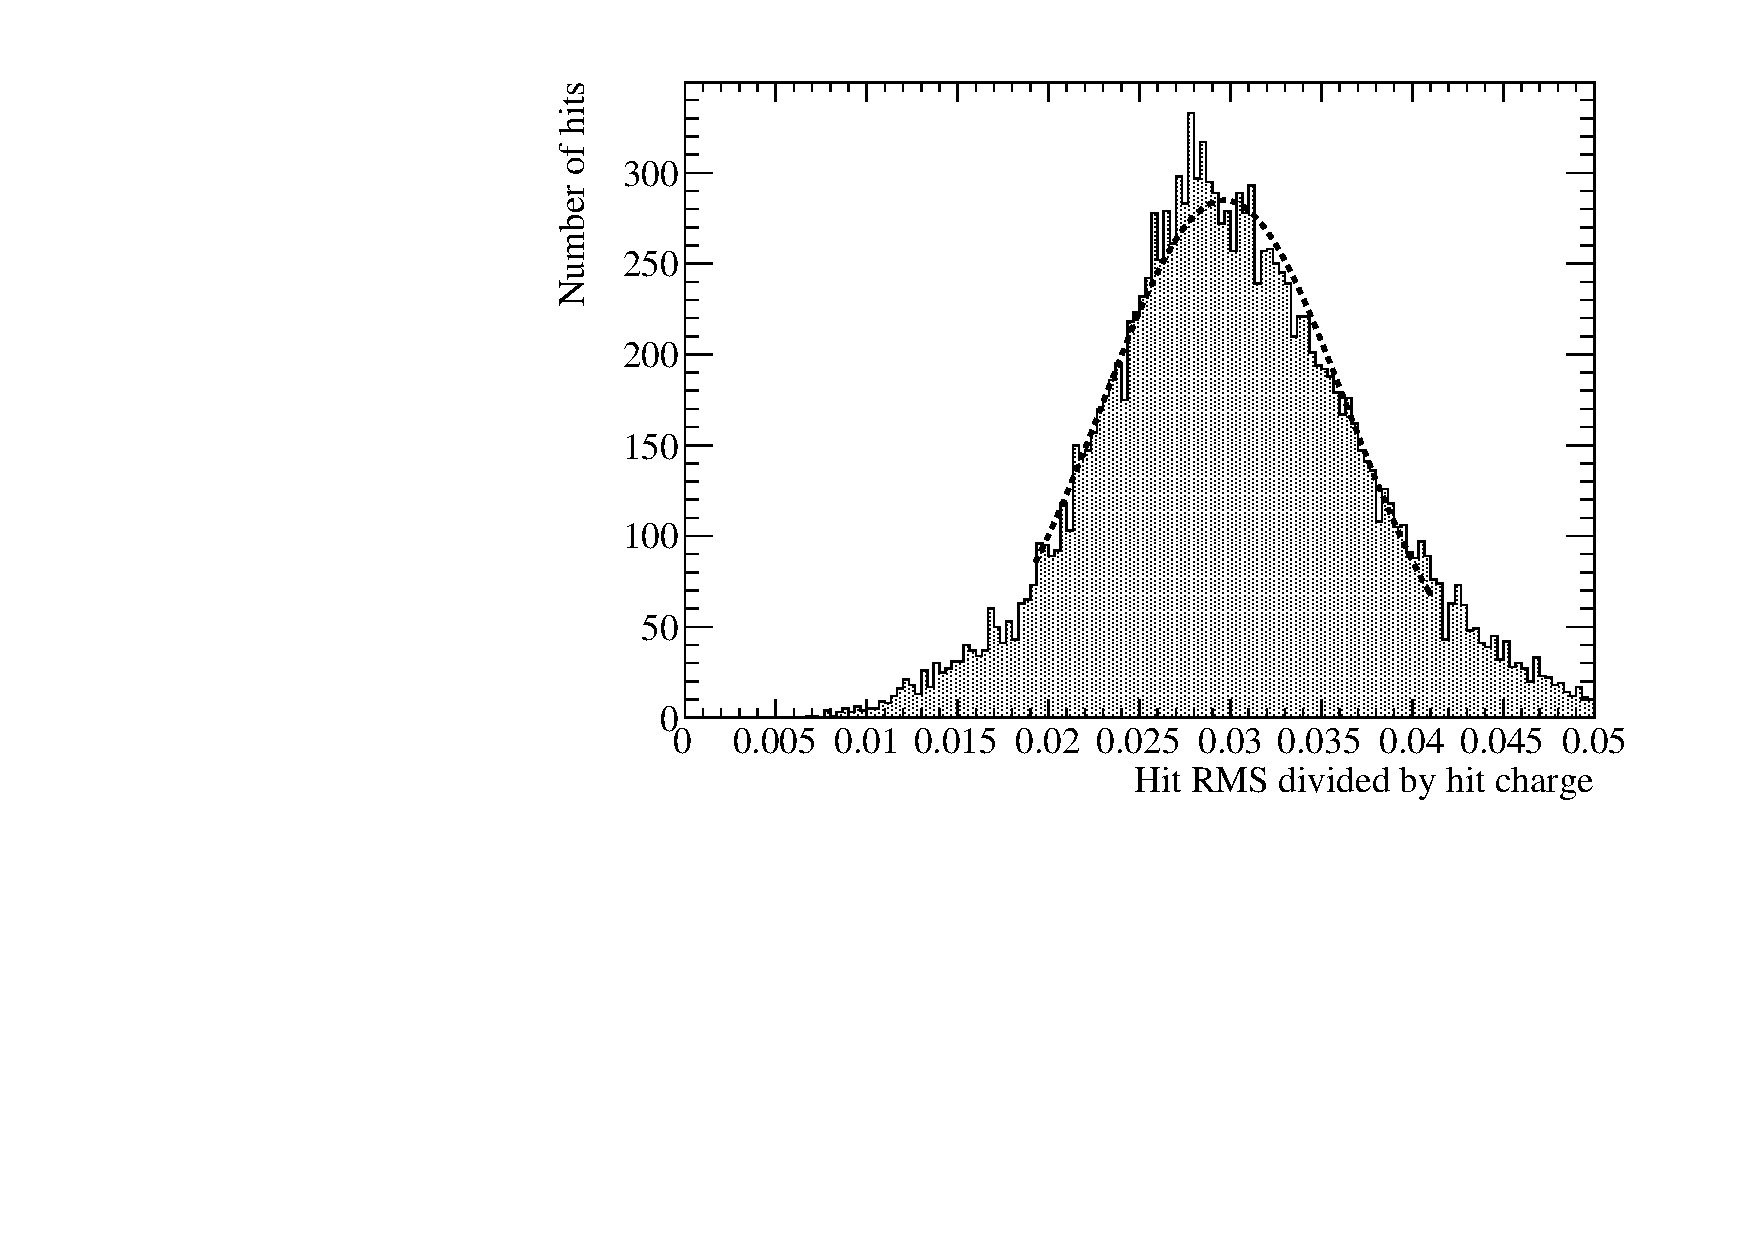
\includegraphics[width=\textwidth]{DataCan_3}
    \caption{The most probable hit $RMS/Charge$ value at $x =$ 140 cm for tracks with a counter difference of 4.}
  \end{subfigure}
  \caption[The most probable values of the $RMS$ and $RMS/Charge$ distributions for tracks with a counter difference of 4 in the 35 ton data]
          {The most probable values for hits from at 20 cm and 140 cm from tracks which triggered a counter difference of 4, when the $RMS$ of the hit and the $RMS/charge$ of the hit are considered.}
          \label{fig:DiffDataHitFit}
\end{figure}

The drift distance effect of diffusion can then be observed for a given range of track angles by fitting these most probable values as drift distance increases. The angular dependence can then be shown by observing how the most probable fit value at a drift distance of 0 cm changes for increasing angles, this is shown in Figure~\ref{fig:DiffDataFit}. A drift distance dependence can clearly be seen in the data as the most probable hit $RMS$ is seen to increase for hits which originate further from the APAs. It also clear that there is an angular dependence on the hit width as the most probable hit widths next to the APAs is seen to rise for tracks which are more inclined relative to the APAs. These dependencies show that when considering a large sample diffusion can be separated into distance and angular dependant dependencies, however whether this can be observed for individual tracks has not yet been considered. \\

\begin{figure}[h!]
  \centering
  \begin{subfigure}{0.45\textwidth}
    \centering
    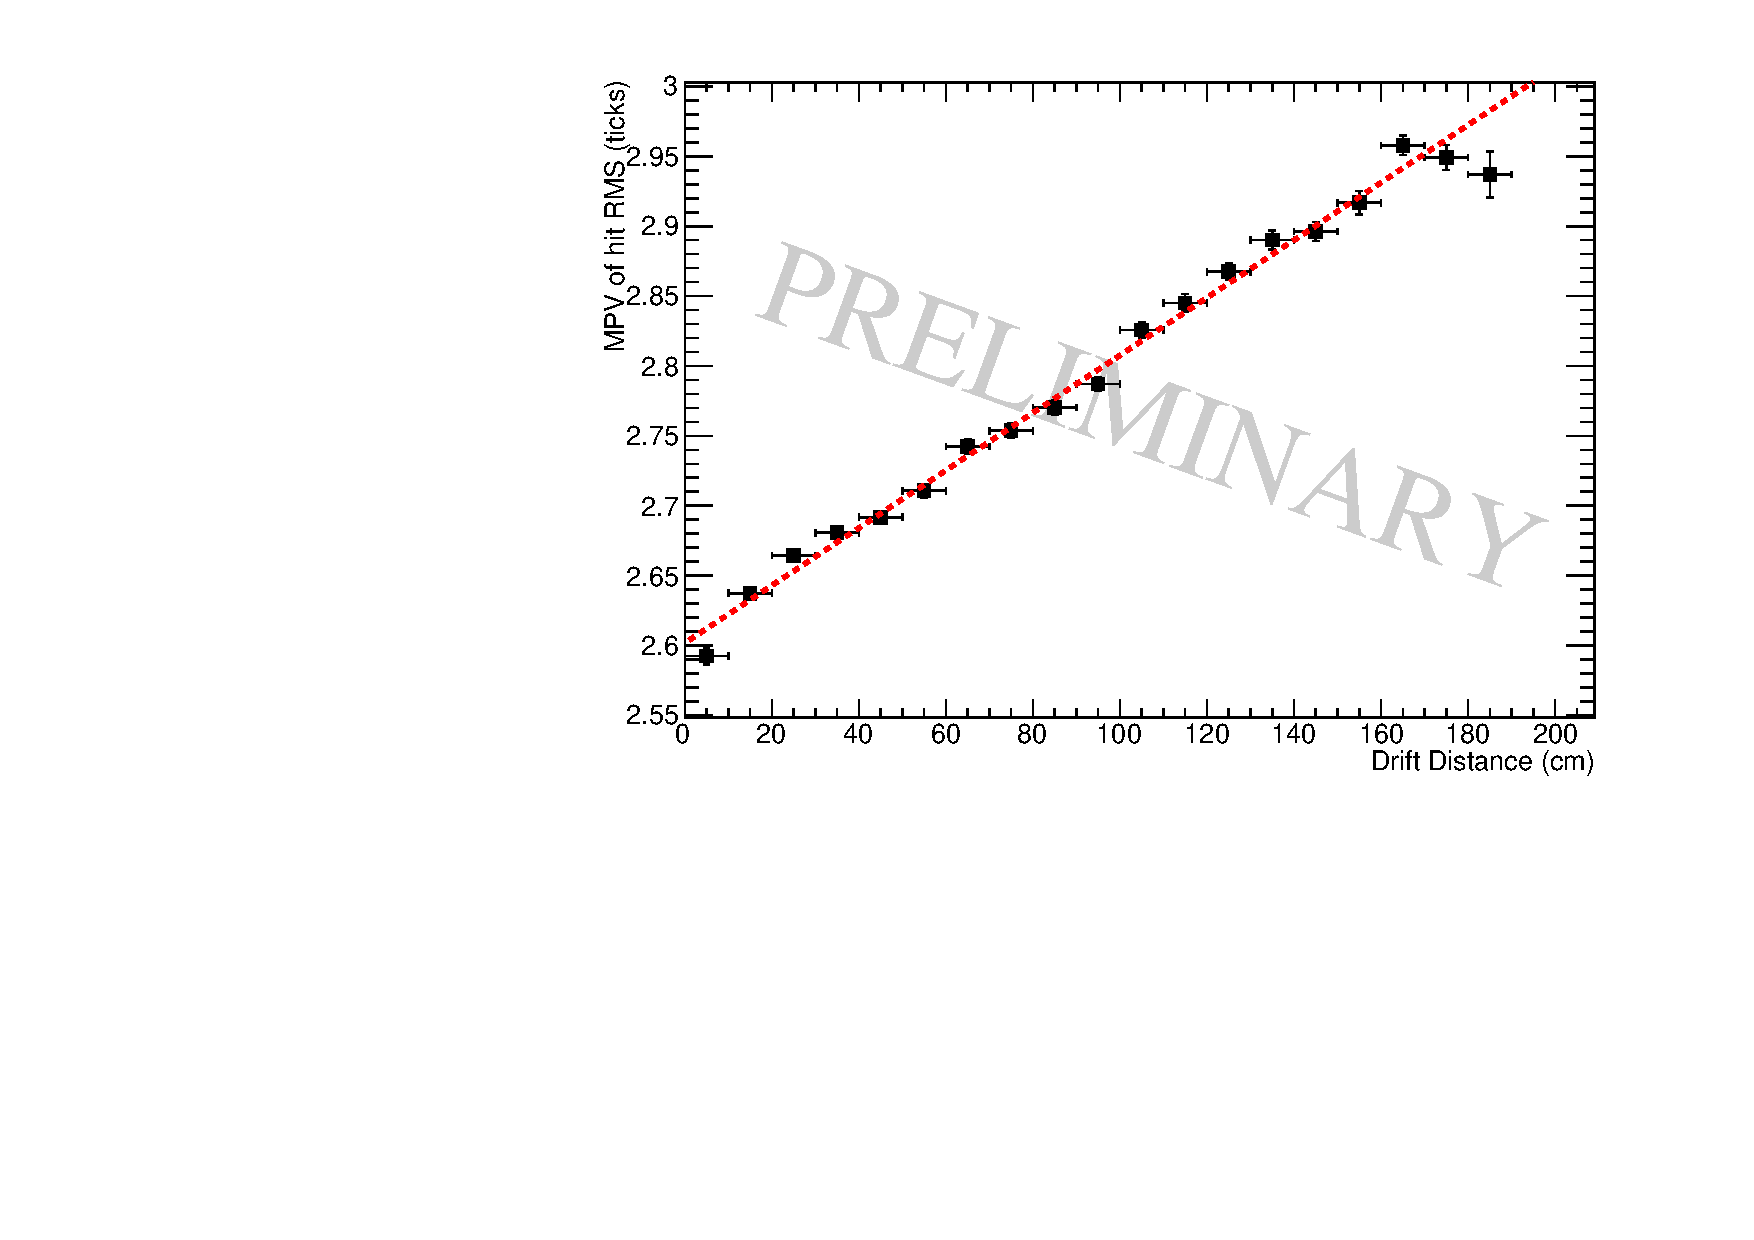
\includegraphics[width=\textwidth]{CounterDiff4_Data}
    \caption{The most probable hit $RMS$ value for tracks with a counter difference of 4 for a range of drift distances.}
    \label{fig:CDiff4DataFit}
  \end{subfigure}
  \hspace{0.08\textwidth}
  \begin{subfigure}{0.45\textwidth}
    \centering
    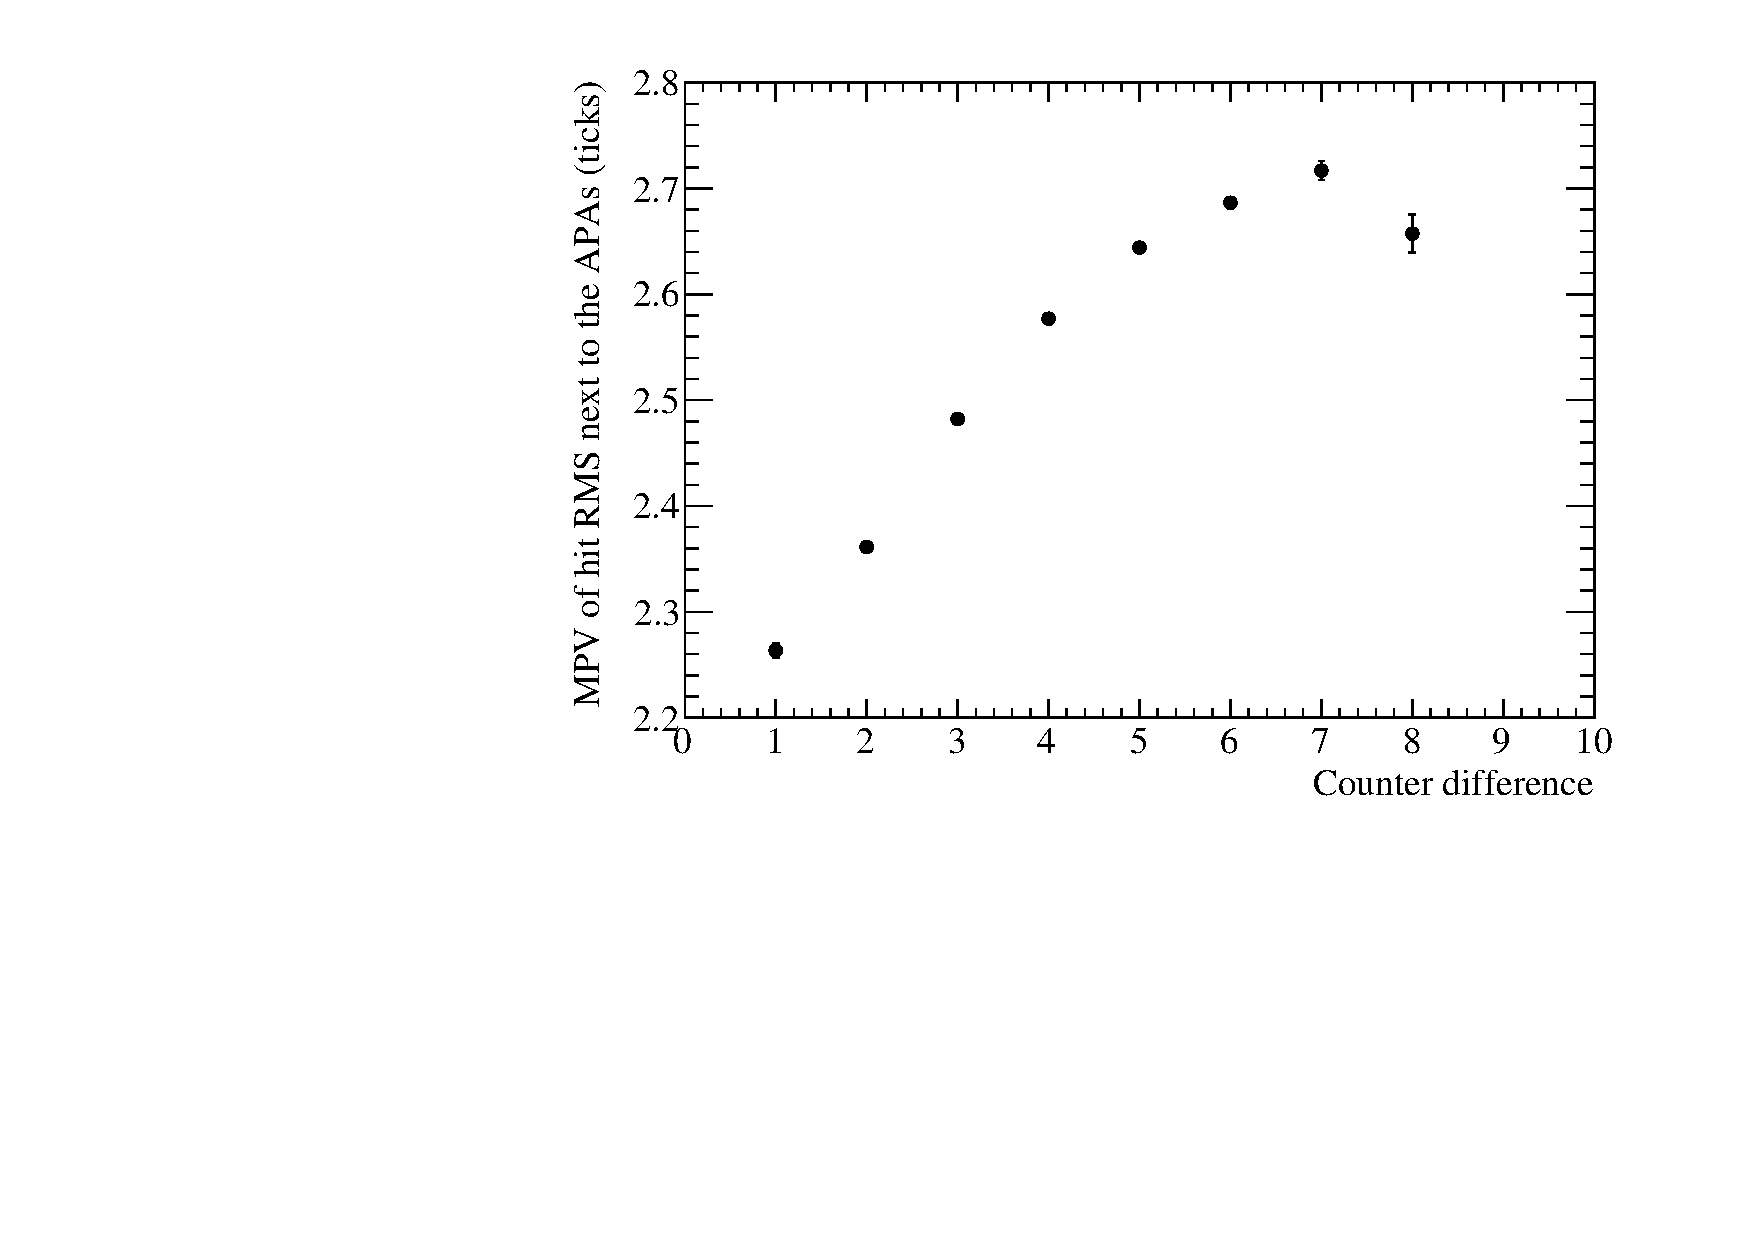
\includegraphics[width=\textwidth]{InterceptCanvasData}
    \caption{The most probable value of hit $RMS$ at a drift distance of 0 cm at increasing track angles.}
  \end{subfigure}
  \caption[The drift distance and angular dependence of diffusion in the 35 ton data]
          {Fits showing the drift distance and angular dependence of diffusion in the 35 ton dataset.}
          \label{fig:DiffDataFit}
\end{figure}

In order to consider single tracks the best line fits for the counter differences for a large sample of tracks, such as in Figure~\ref{fig:CDiff4DataFit}, need to be used to predict the drift position you would expect a hit to originate from given a value for its hit $RMS$ and the angle of track to which it belongs. The predicted positions can then be compared to the known position from the counter co-incidence to determine the accuracy of the prediction. As the distributions shown in Figure~\ref{fig:DiffDataHitFit} are roughly symmetric around the most probable value one would naively expect that if a track has a sufficient number of hits then the distribution of RMS values for those hits would match that found over a large sample. If this were to be the case then the difference in reconstructed and predicted hit times should be peaked around the track interaction time. \\

An intrinsic assumption in this method is that the track has a large number of collection plane hits that do not contain delta rays and are on wires which would not be identified as noisy. The tracks being considered will have crossed all $z$ values in the detector meaning that a total of 336 collection hits could potentially be reconstructed. Given the reconstruction problems in the 35 ton very few tracks will have hits on all of these collection wires, however requiring at least 100 collection plane hits is not unreasonable and would correspond to a reconstructed track length of at least 50 cm. The predicted hit times and the difference in predicted and reconstructed hit times are shown in Figure~\ref{fig:DiffDataPredHit} for both prediction metrics. It can be seen that in the 35 ton dataset the $RMS/Charge$ metric appears to provide a more robust measurement of the interaction time as the peak value for the predicted minus reconstructed hit time is more closely centred around 0 and is much larger than for the RMS metric. The peak is centred around a difference of 0 as the hits had previously been corrected so as to be centred around the measured interaction time from the counter coincidence. \\

\begin{figure}[h!]
  \centering
  \begin{subfigure}{0.45\textwidth}
    \centering
    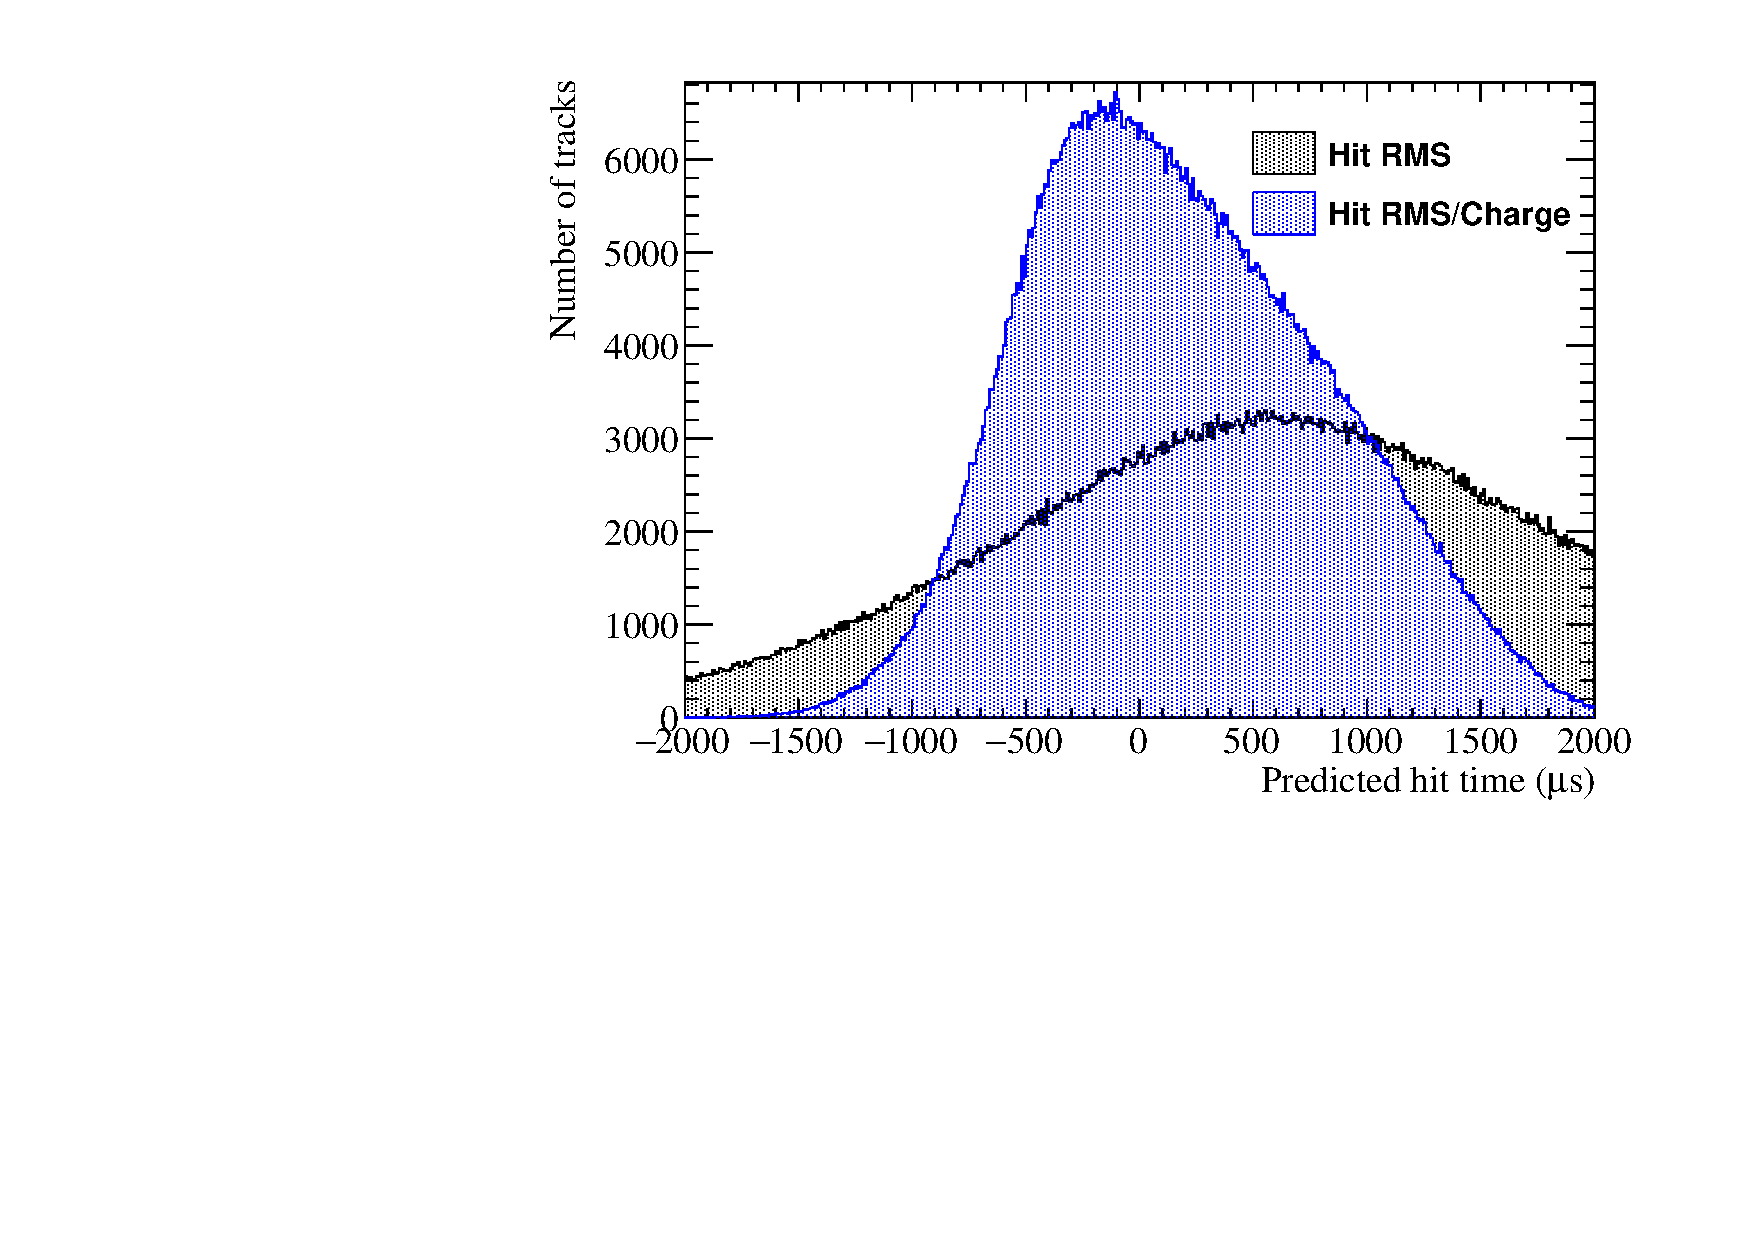
\includegraphics[width=\textwidth]{PredictedInteractionTime_Data}
    \caption{The predicted hit time for each hit in all tracks with more than 100 'good' collection plane hits.}
  \end{subfigure}
  \hspace{0.08\textwidth}
  \begin{subfigure}{0.45\textwidth}
    \centering
    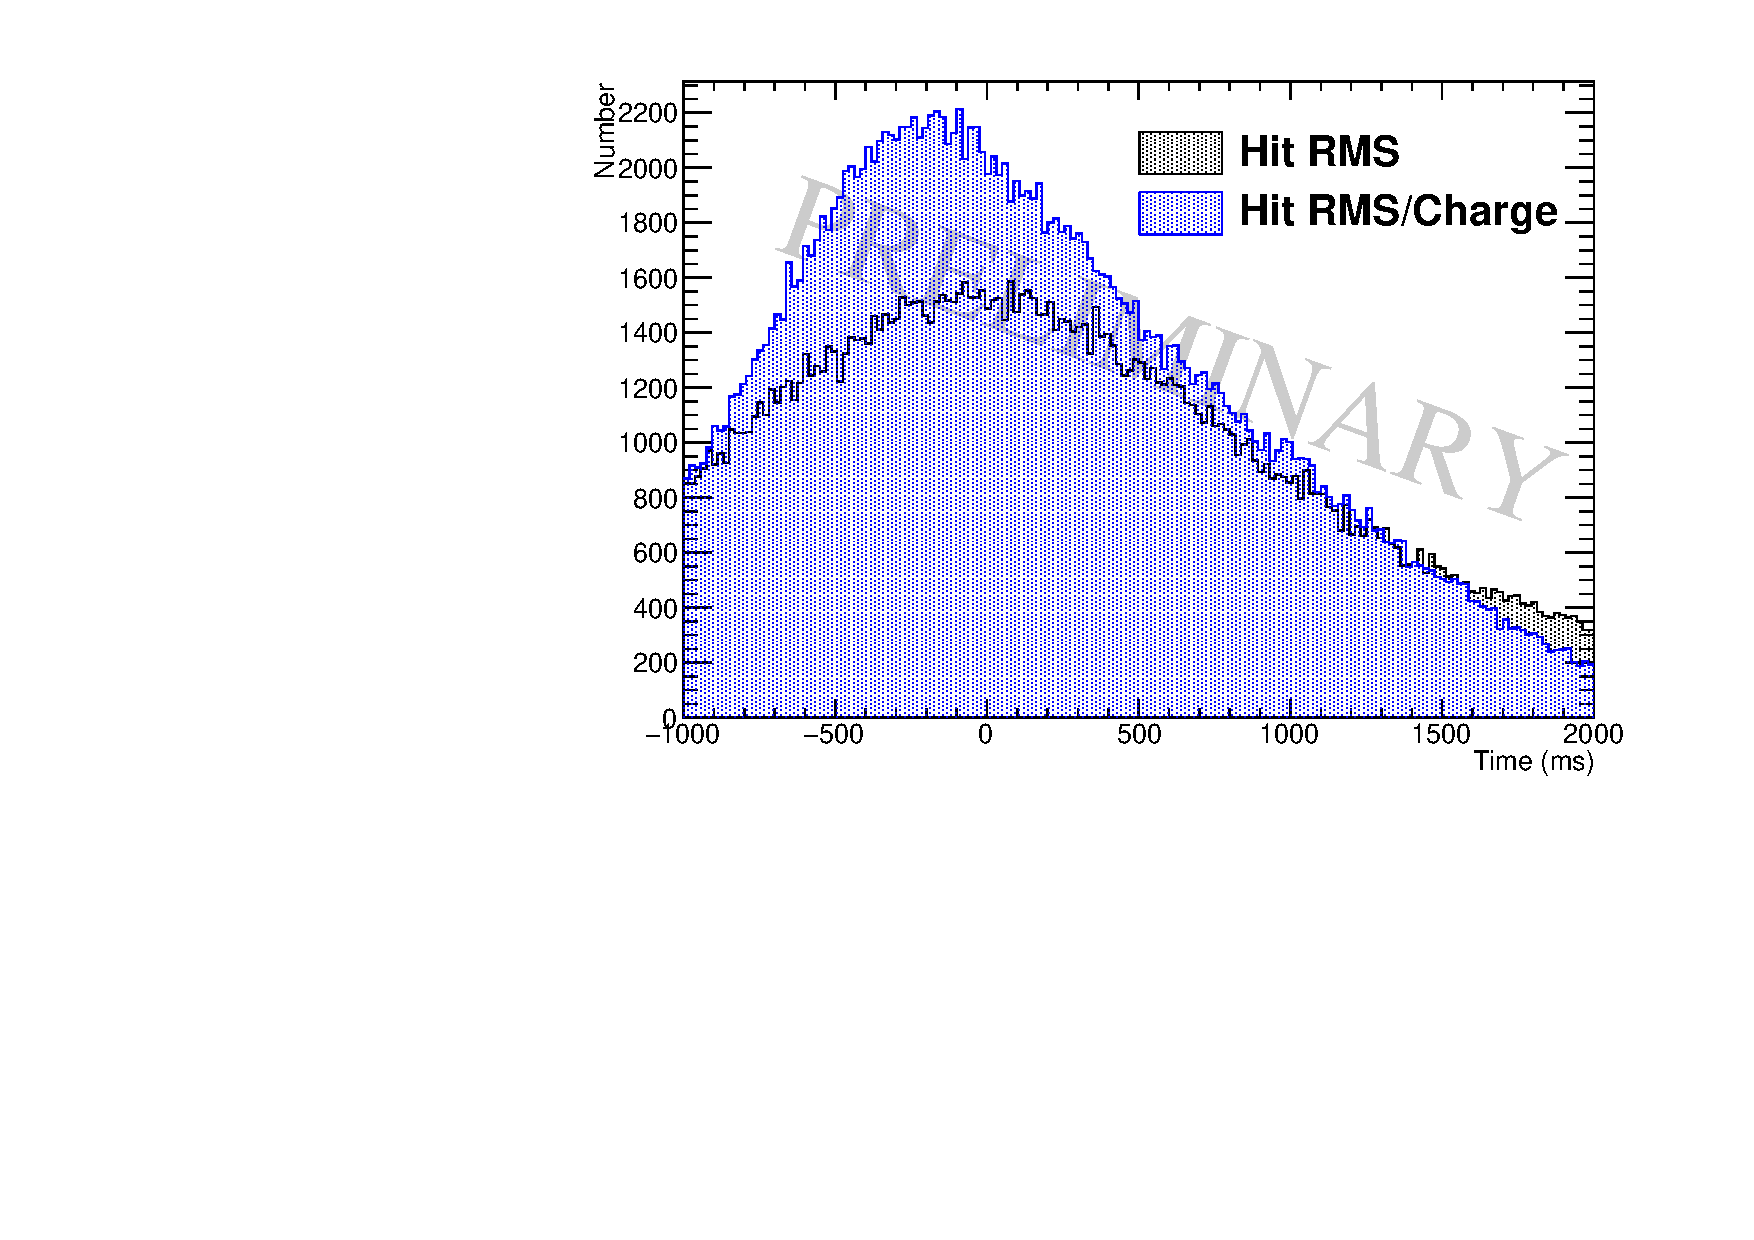
\includegraphics[width=\textwidth]{DifferenceInteractionTime_Data}
    \caption{The difference in reconstructed and predicted hit time for each hit in all tracks with more than 100 'good' collection plane hits.}
  \end{subfigure}
  \caption[The predicted hit times for tracks with more than 100 'good' hit collection plane hits in the 35 ton data]
          {The predicted hit times for tracks with more than 100 'good' hit collection plane hits in the 35 ton data. The times predicted by the hit $RMS$ metric are shown in black, whilst the times predicted by the hit $RMS/Charge$ metric are shown in blue.}
          \label{fig:DiffDataPredHit}
\end{figure}

When evaluating interaction times the average difference in reconstructed and predicted hit times across every hit on the track must be considered. This is shown in Figure~\ref{fig:DiffDataAvDiff}, where as expected from Figure~\ref{fig:DiffDataPredHit} the $RMS/Charge$ metric provides a better estimation of the interaction time. The reason for this is that by utilising the charge information due to losses from impurities this metric gains an extra handle on the drift distance and hence the reconstructed time of the hits. The losses due to impurities are difficult to measure in very high purity LAr environments though as the decrease in collected charge at increasing drift distances becomes small~\citep{LongBo}. The effect of increasing LAr purity is shown in Section~\ref{sec:DiffMCStudies}. Using the change in hit charge in the 35 ton is not without its own dangers though, because as shown in Figure~\ref{fig:TingjunLifetime} there is a thresholding effect for hits with large drift times. However, as the same thresholding effect is present in all 35 ton data samples the limitation it introduces is mainly in the efficiency with which 'good' collection plane hits will be reconstructed and so this information can be confidently used. \\

\begin{figure}[h!]
  \centering
  \begin{subfigure}{0.45\textwidth}
    \centering
    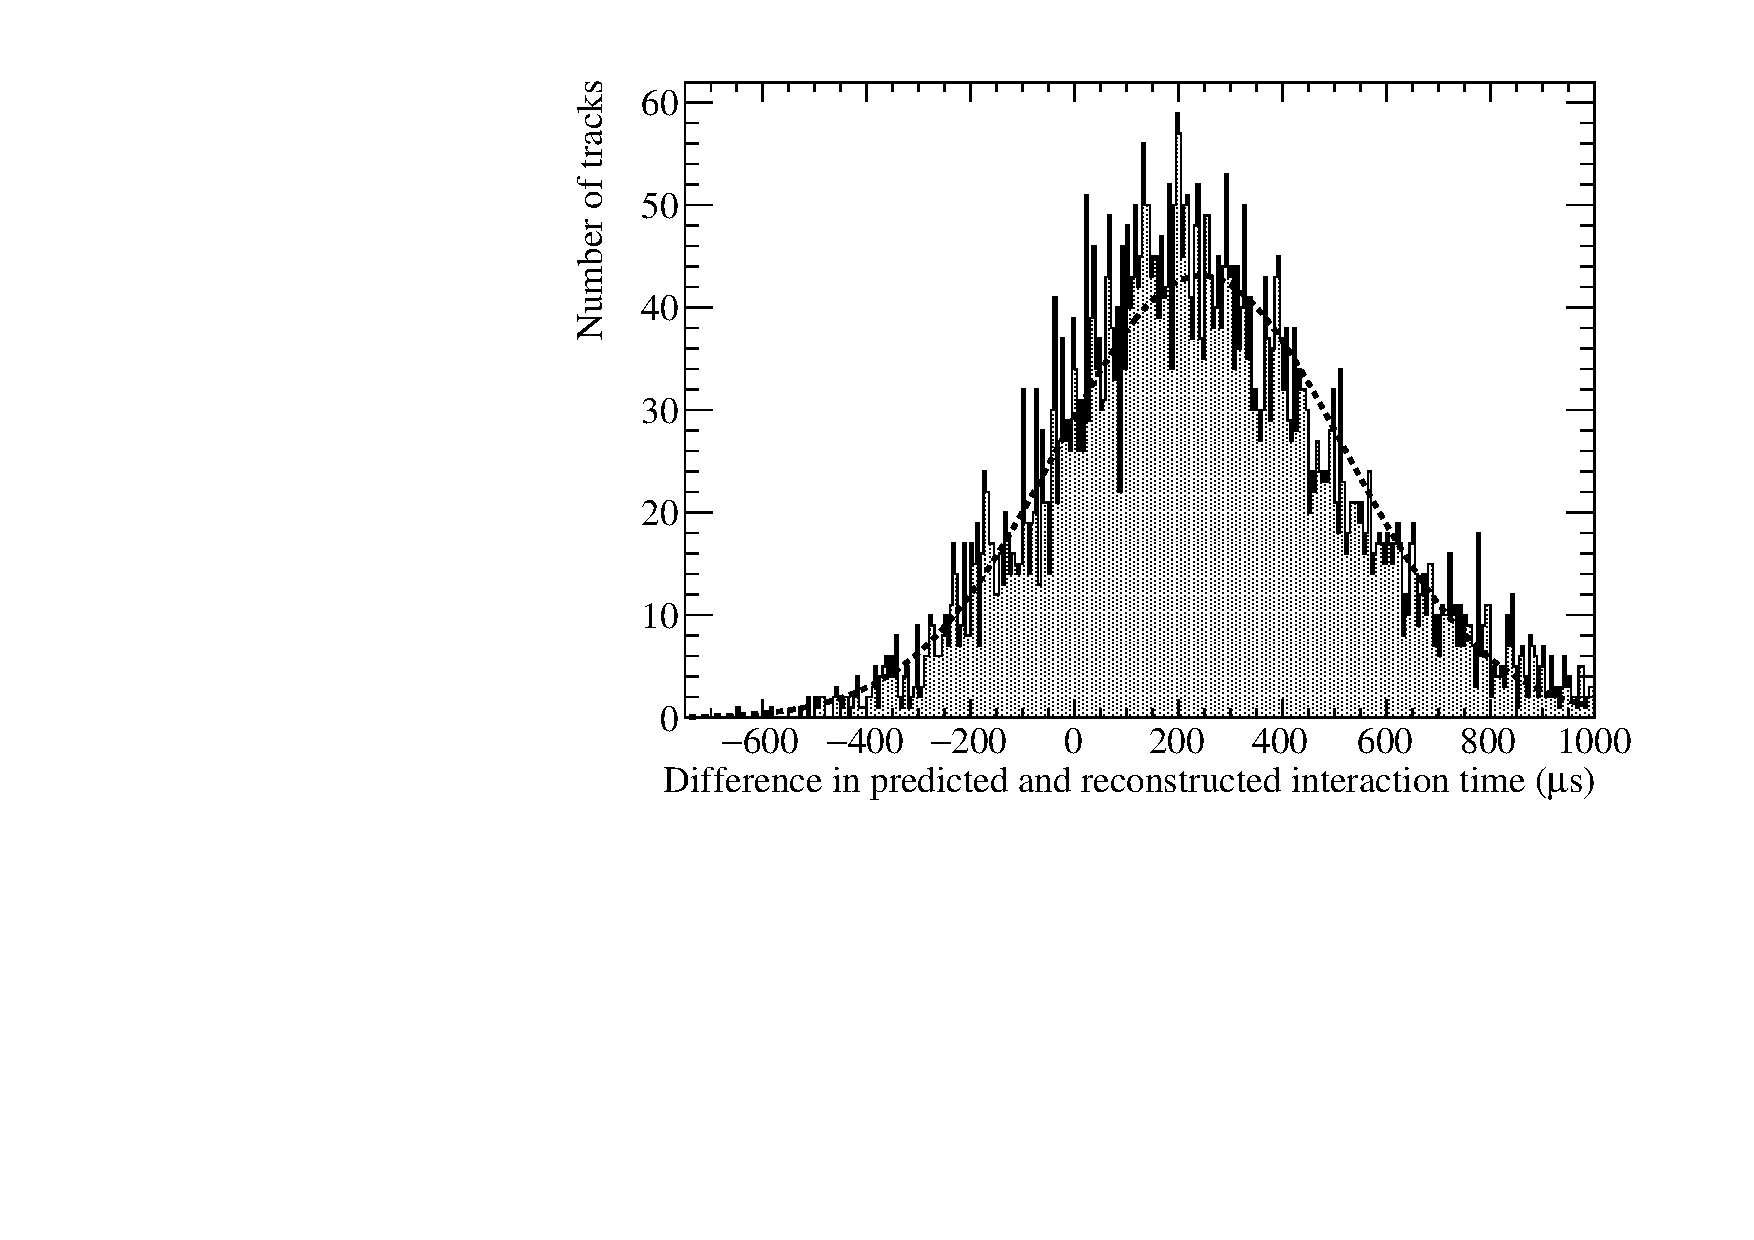
\includegraphics[width=\textwidth]{Data_AvTimeDiff_RMS}
    \caption{The average difference in interaction times using the hit $RMS$ metric.}
  \end{subfigure}
  \hspace{0.08\textwidth}
  \begin{subfigure}{0.45\textwidth}
    \centering
    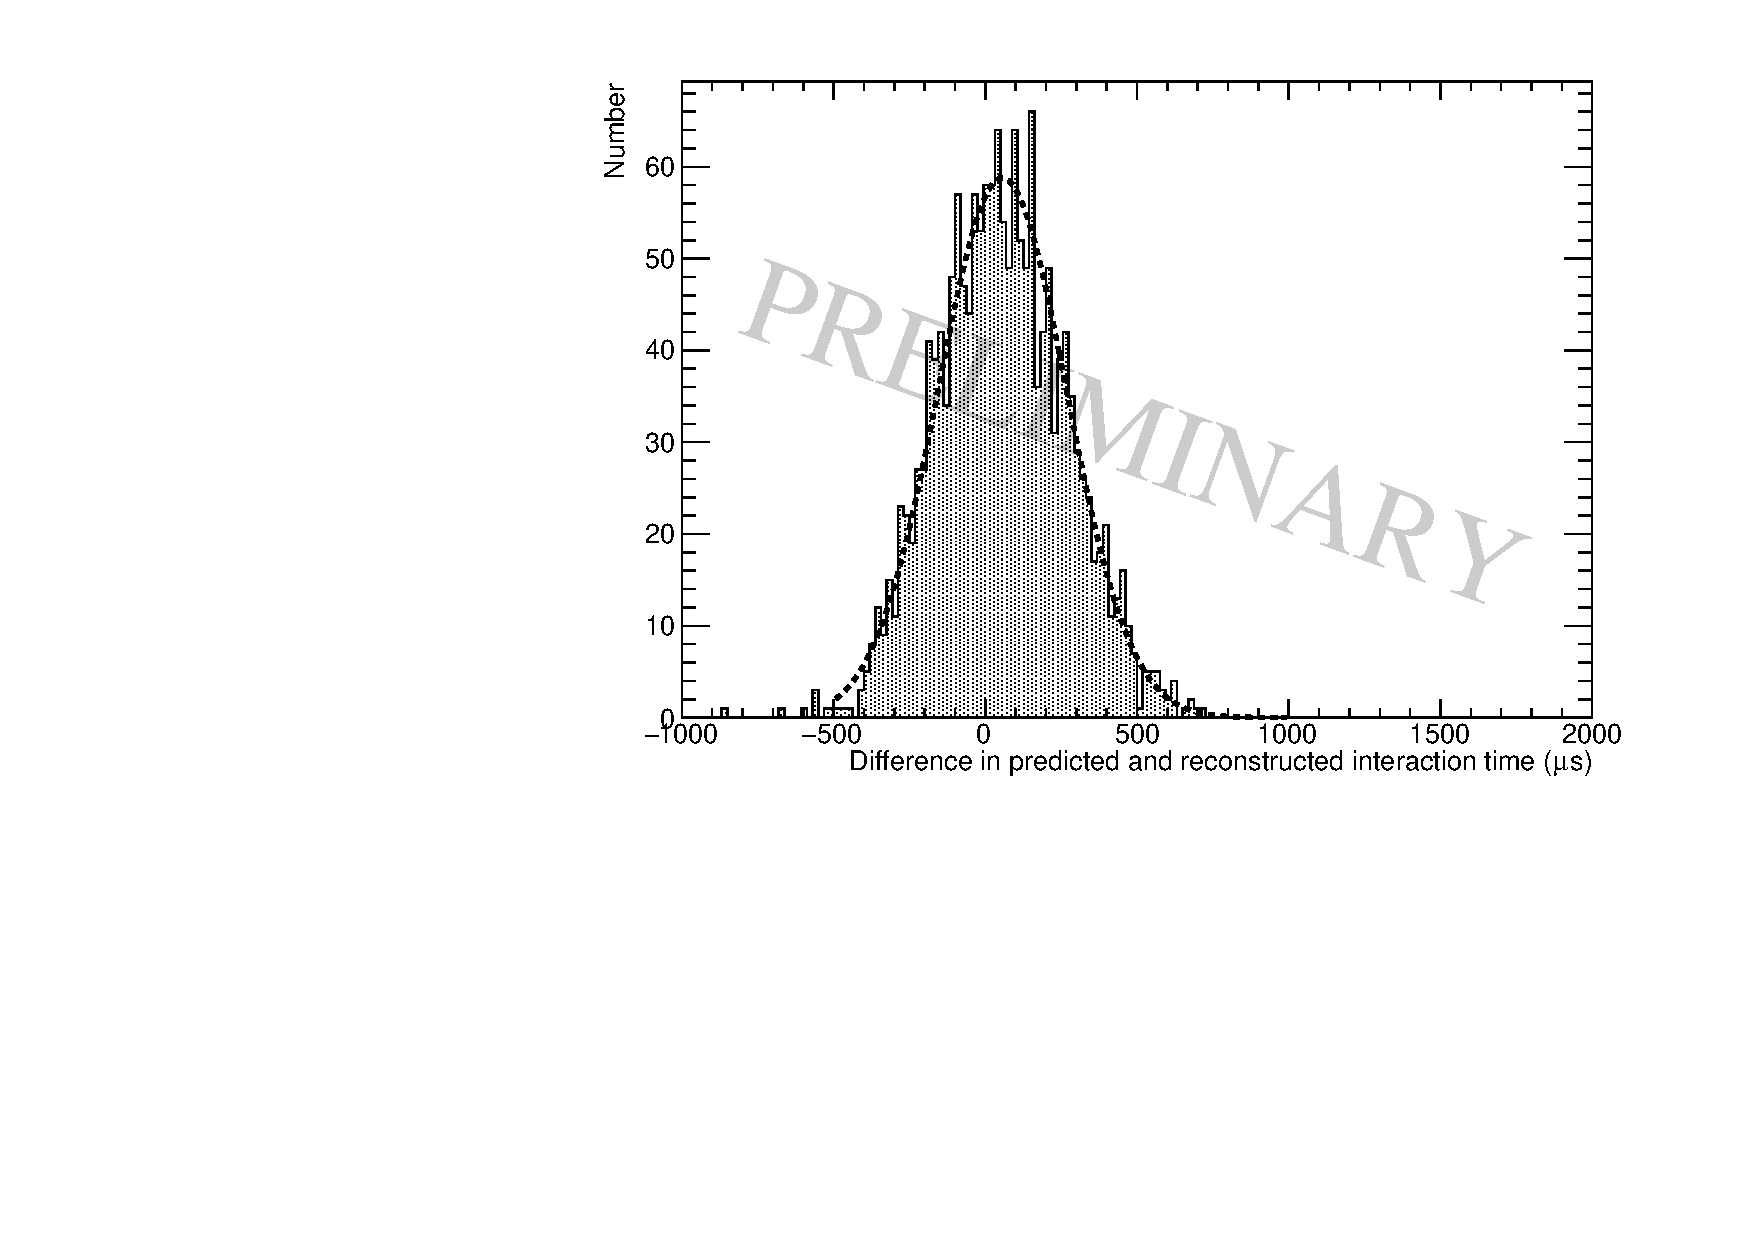
\includegraphics[width=\textwidth]{Data_AvTimeDiff_RMS_Int}
    \caption{The average difference in interaction times using the hit $RMS/Charge$ metric.}
  \end{subfigure}
  \caption[The difference in predicted and reconstructed interaction times in the 35 ton data]
          {The difference in predicted and reconstructed interaction times in the 35 ton data.}
          \label{fig:DiffDataAvDiff}
\end{figure}

Figure~\ref{fig:DiffDataAvDiff} shows that the interaction time of a reconstructed track in the 35 ton dataset can be determined using the effects of diffusion to an accuracy of 298.0$\pm$267.0 $\mu$s when using the hit $RMS$ metric and to an accuracy of 55.6$\pm$210.4 $\mu$s when using the hit $RMS/Charge$ metric. This resolution is impressive as even with the issues with regards to data quality in the 35 ton tracks can be cleanly separated throughout a drift window of 5200 $\mu$s. The application of the method to a low noise environment would provide the true accuracy of the method, because one would expect that the problems with data quality would adversely affect the accuracy to which diffusion can be measured. For this reason the next section presents a complementary analysis performed on a low background sample of 35 ton Monte Carlo with the same electronics settings as the data presented here. 

%********************************** % Fifth.Second Section  *************************************
\subsection{Determining interaction times in a low noise detector and differences with data}
When determining interaction times in an ideal detector exactly the same criteria are applied to the hits, as delta rays would still change the measured hit width and will be present in any sample. In a low noise detector it is expected that few wires would be removed due to being noisy but for consistency there is no danger in applying this cut. Imposing a minimum number of collection plane hits is again important to ensure that the distribution of predicted hit times is centred on the interaction time. In addition to the same criteria being imposed on which wires are used, the same metrics are calculated. In all plots shown below the Monte Carlo dataset has been normalised to the size of the 35 ton dataset. \\

Figure~\ref{fig:DiffMCHitFit} shows both the $RMS$ and $RMS/Charge$ distributions for hits that are 100 cm away from the APAs and are from tracks with a counter difference of 4. It can be seen that the distributions from the low noise Monte Carlo are tighter than those from the 35 ton data and are also peaked at a lower hit RMS. This is likely due to the fact that the coherent noise baseline seen in data can increase the width of hits as shown in Figure~\ref{fig:DomsHitModel} and a higher noise state will affect how well individual hits can be reconstructed. In addition, the most probable values of hit $RMS$ at increasing drift distance is shown in Figure~\ref{fig:DiffMCDataCompFit} where the low noise Monte Carlo is again shown against the values from the data. The most probable value of hit $RMS$ at a drift distance of 0 cm for a range of angles is also shown in Figure~\ref{fig:DiffMCDataCompInt}. As was seen when considering the distributions at specific distances and angles the most probable hit $RMS$ in the low noise Monte Carlo is systematically lower than in the data due to the elevated noise level in the data. Another difference between the Monte Carlo and the data is that the gradient of the most probable hit $RMS$ values in data is roughly half of that in the Monte Carlo, this could be due to an overestimation of longitudinal diffusion in the Monte Carlo. \\

\begin{figure}[h!]
  \centering
  \begin{subfigure}{0.45\textwidth}
    \centering
    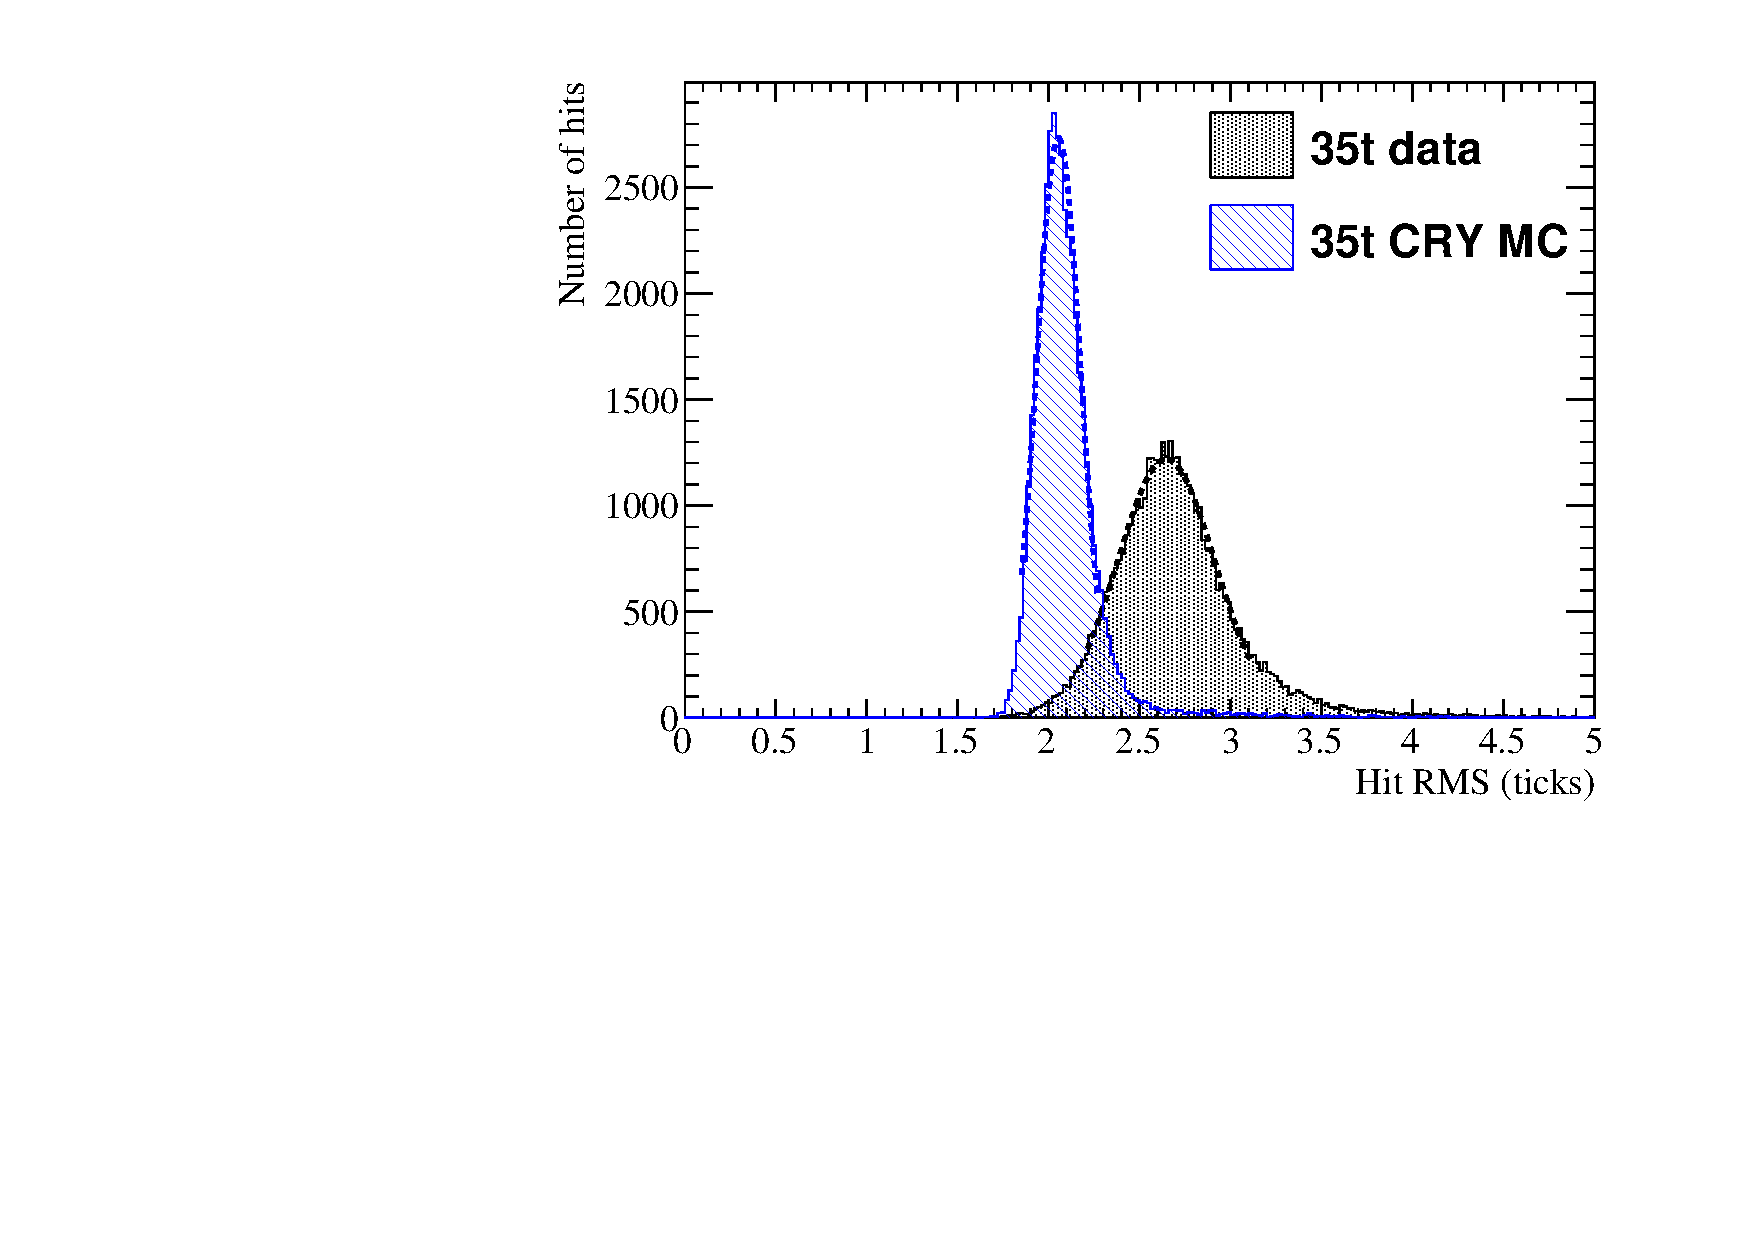
\includegraphics[width=\textwidth]{CombCan_0}
    \caption{The distribution of hit $RMS$ values at $x =$ 20 cm.}
  \end{subfigure}
  \hspace{0.08\textwidth}
  \begin{subfigure}{0.45\textwidth}
    \centering
    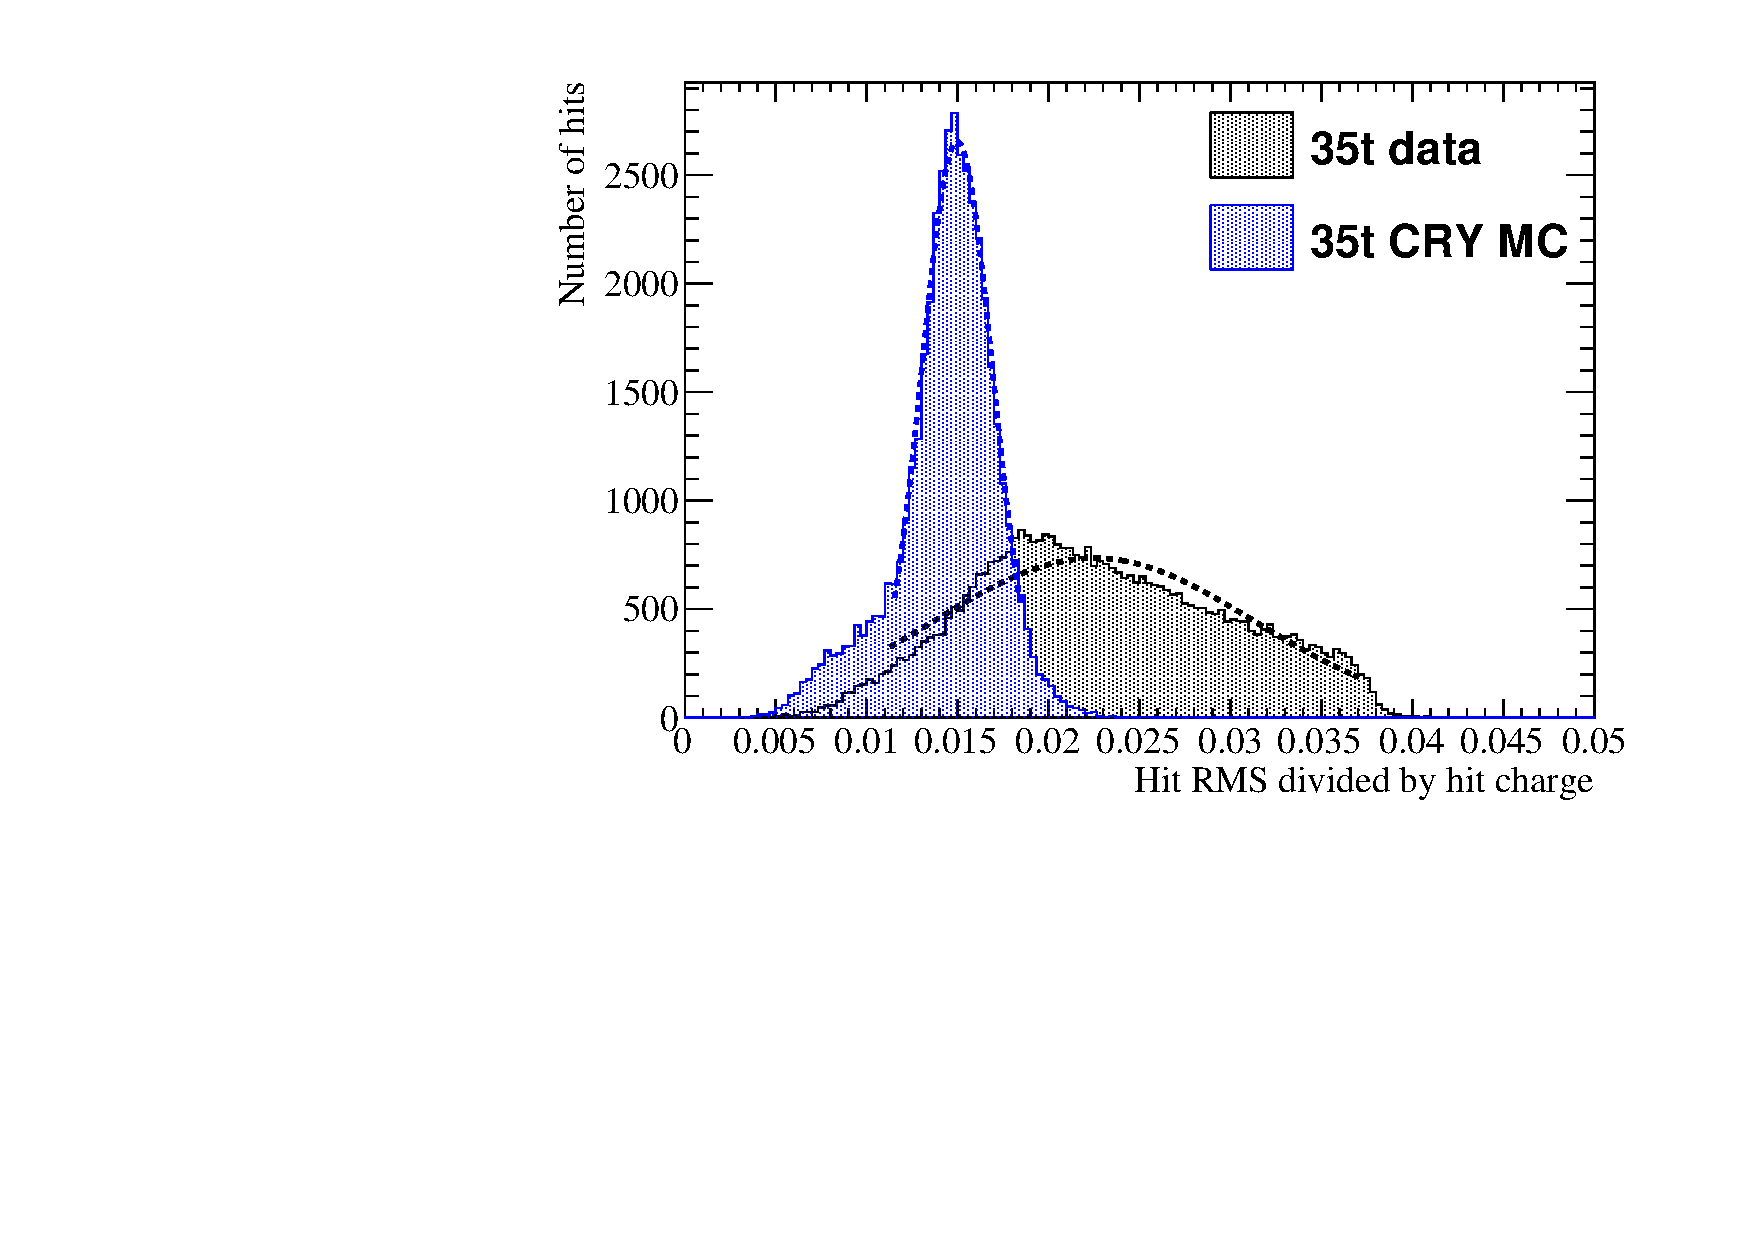
\includegraphics[width=\textwidth]{CombCan_2}
    \caption{The distribution of hit $RMS/Charge$ values at $x =$ 20 cm.}
  \end{subfigure}
  \caption[The most probable values of the $RMS$ and $RMS/Charge$ distributions for tracks with a counter difference of 4 in a low noise 35 ton detector]
          {The most probable values of the $RMS$ and $RMS/Charge$ distributions at $x =$ 20 cm for tracks with a counter difference of 4. The distributions from the 35 ton data are shown in black, whilst the distributions from the low noise simulation are shown in blue.}
          \label{fig:DiffMCHitFit}
\end{figure}

\begin{figure}[h!]
  \centering
  \begin{subfigure}{0.45\textwidth}
    \centering
    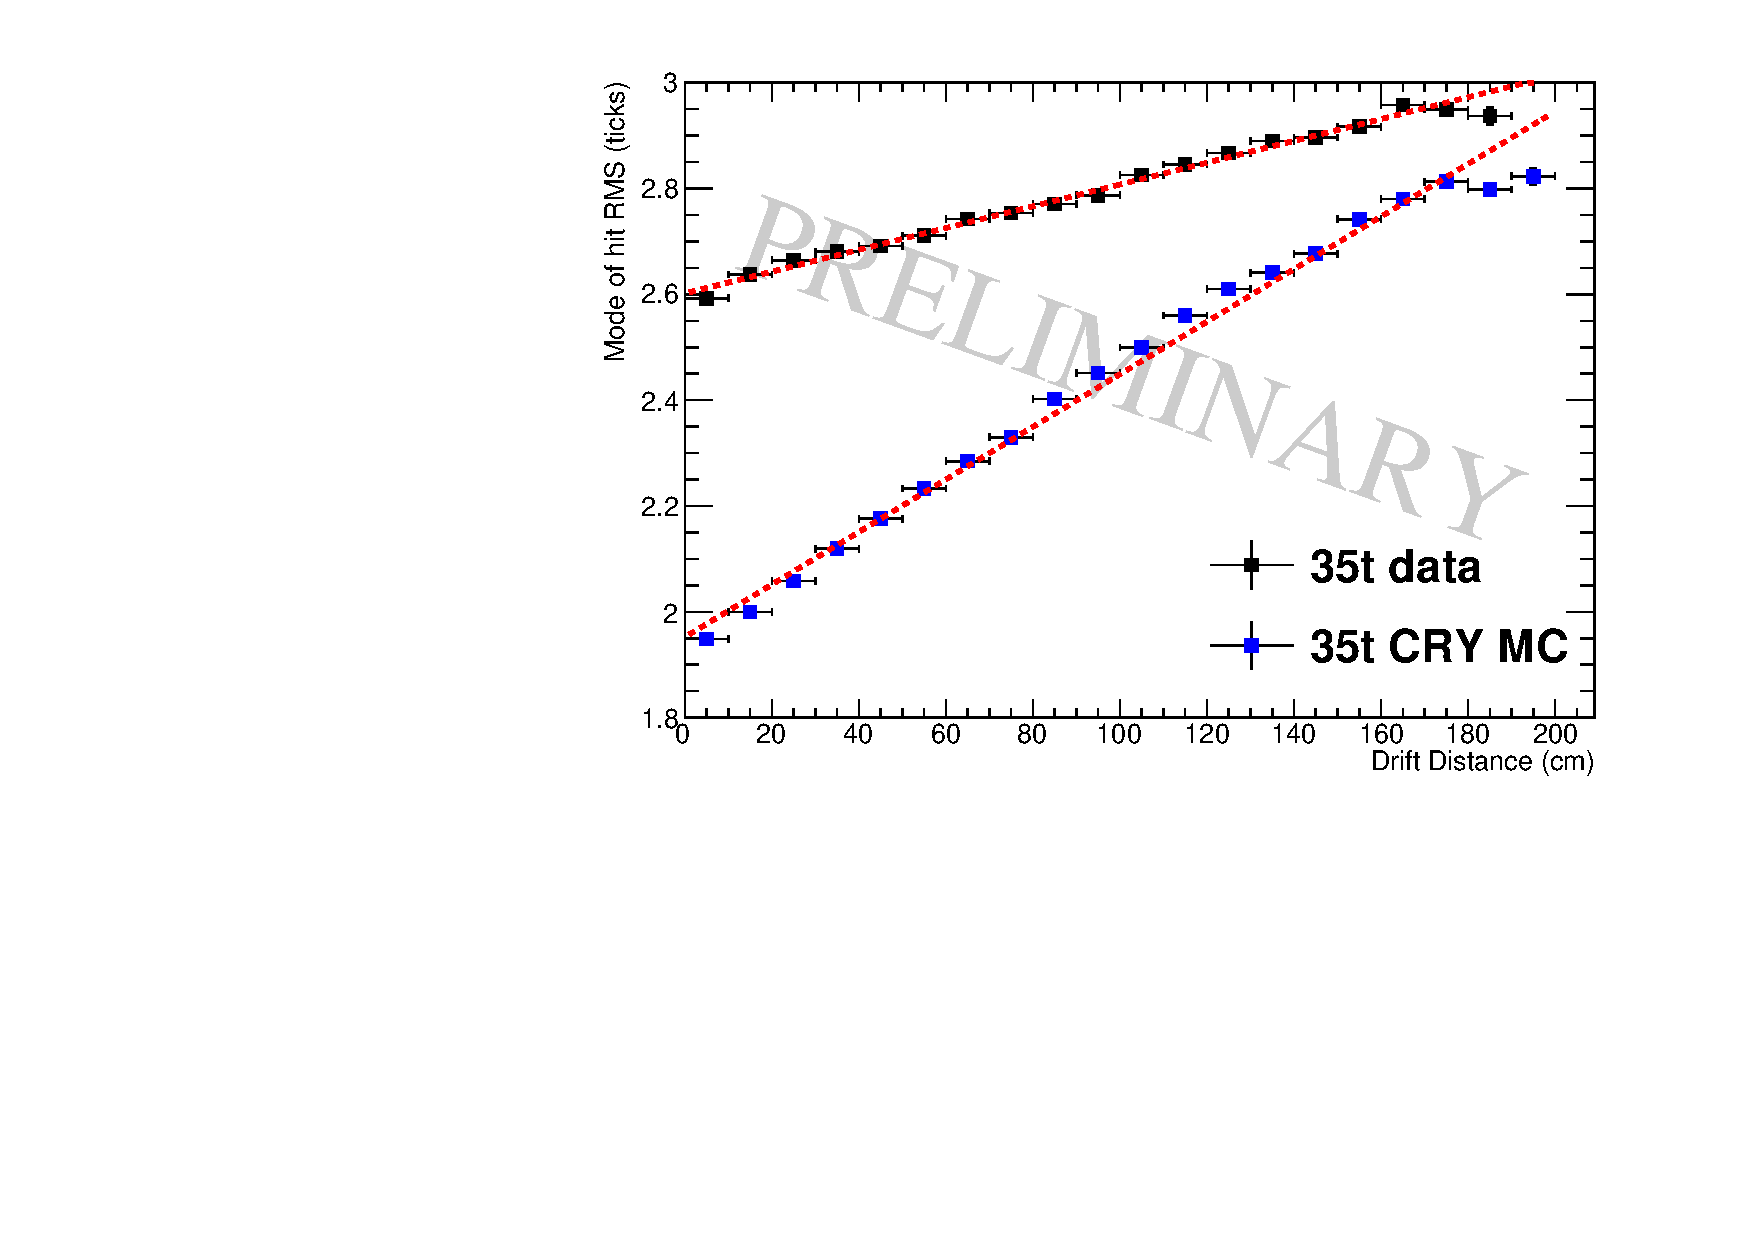
\includegraphics[width=\textwidth]{CounterDiff4_Overlay}
    \caption{The most probable hit $RMS$ values for tracks with a counter difference of 4.}
    \label{fig:DiffMCDataCompFit}
  \end{subfigure}
  \hspace{0.08\textwidth}
  \begin{subfigure}{0.45\textwidth}
    \centering
    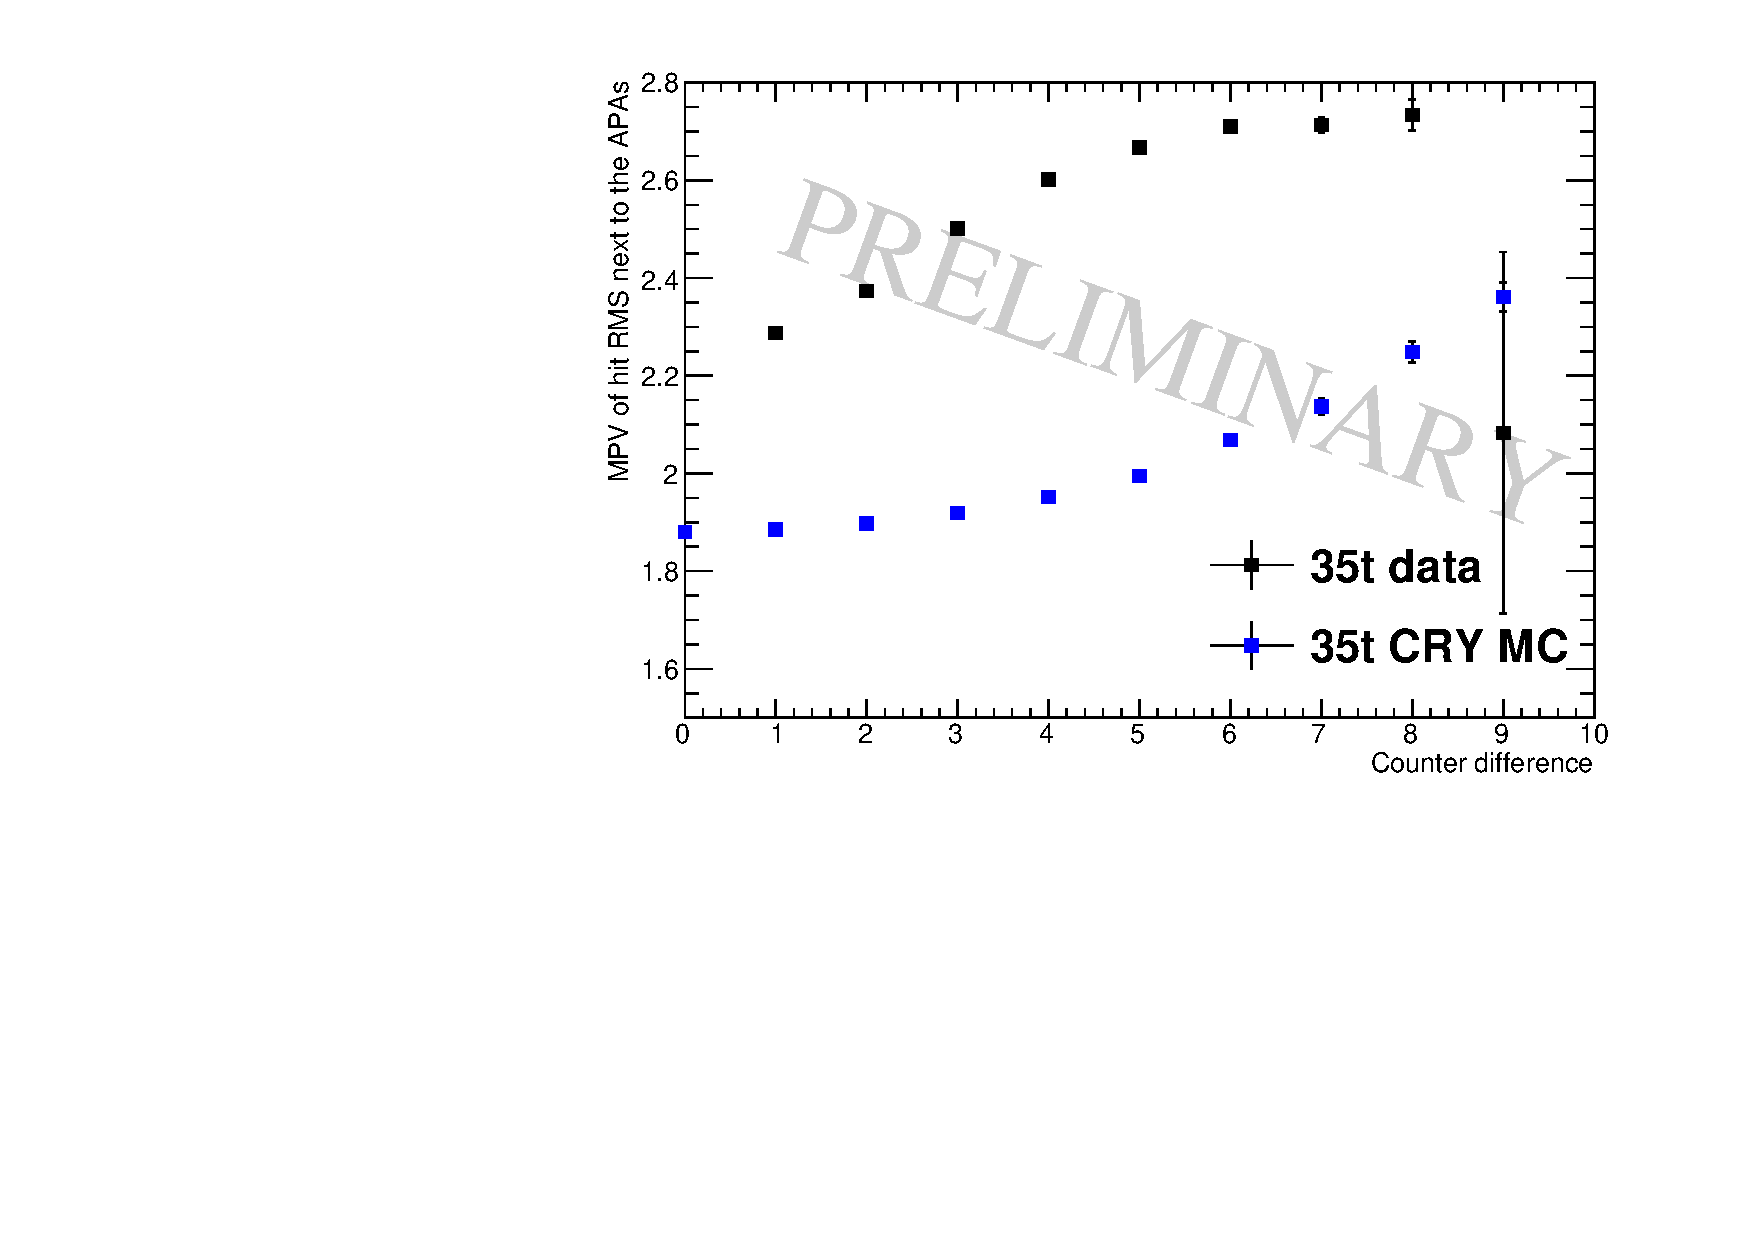
\includegraphics[width=\textwidth]{InterceptCanvasOverlay}
    \caption{The most probable hit $RMS$ values at $x = $ 0 for a range of track angles.}
    \label{fig:DiffMCDataCompInt}
  \end{subfigure}
  \caption[Comparison of the drift distance and angular dependence of diffusion in a low noise 35 ton detector and the 35 ton dataset]
          {A comparison of the drift distance and angular dependence of diffusion in a low noise 35 ton detector and the 35 ton dataset. The distributions from the 35 ton data are shown in black, whilst the distributions from the low noise simulation are shown in blue.}
          \label{fig:DiffMCDataComp}
\end{figure}

Upon calculating the fit metrics in the low noise Monte Carlo sample it is then possible to use these to predict track interaction times, this is shown in Figure~\ref{fig:DiffMCDataRes}. As observed when considering the data sample, the $RMS/Charge$ metric appears to be better able to accurately predict interaction times, this is again due to the ability to incorporate information about loses due to impurities which increase with drift distance. Also, as expected from the previous figures and the lower noise state in the Monte Carlo it is seen that the interaction times predicted in the Monte Carlo more closely match the true interaction times than in the data. The accuracy of interaction time determination in Monte Carlo (data) is shown to be 168.1$\pm$126.5 (298.0$\pm$267.0) $\mu$s and -41.2$\pm$107.8 (55.6$\pm$210.4) $\mu$s for the hit $RMS$ and $RMS/Charge$ metrics respectively. An important feature to observe is that the widths of the distributions in Monte Carlo is less than half of that in the data, again this is attributed to the lower noise level in the Monte Carlo.

\begin{figure}[h!]
  \centering
    \begin{subfigure}{0.45\textwidth}
    \centering
    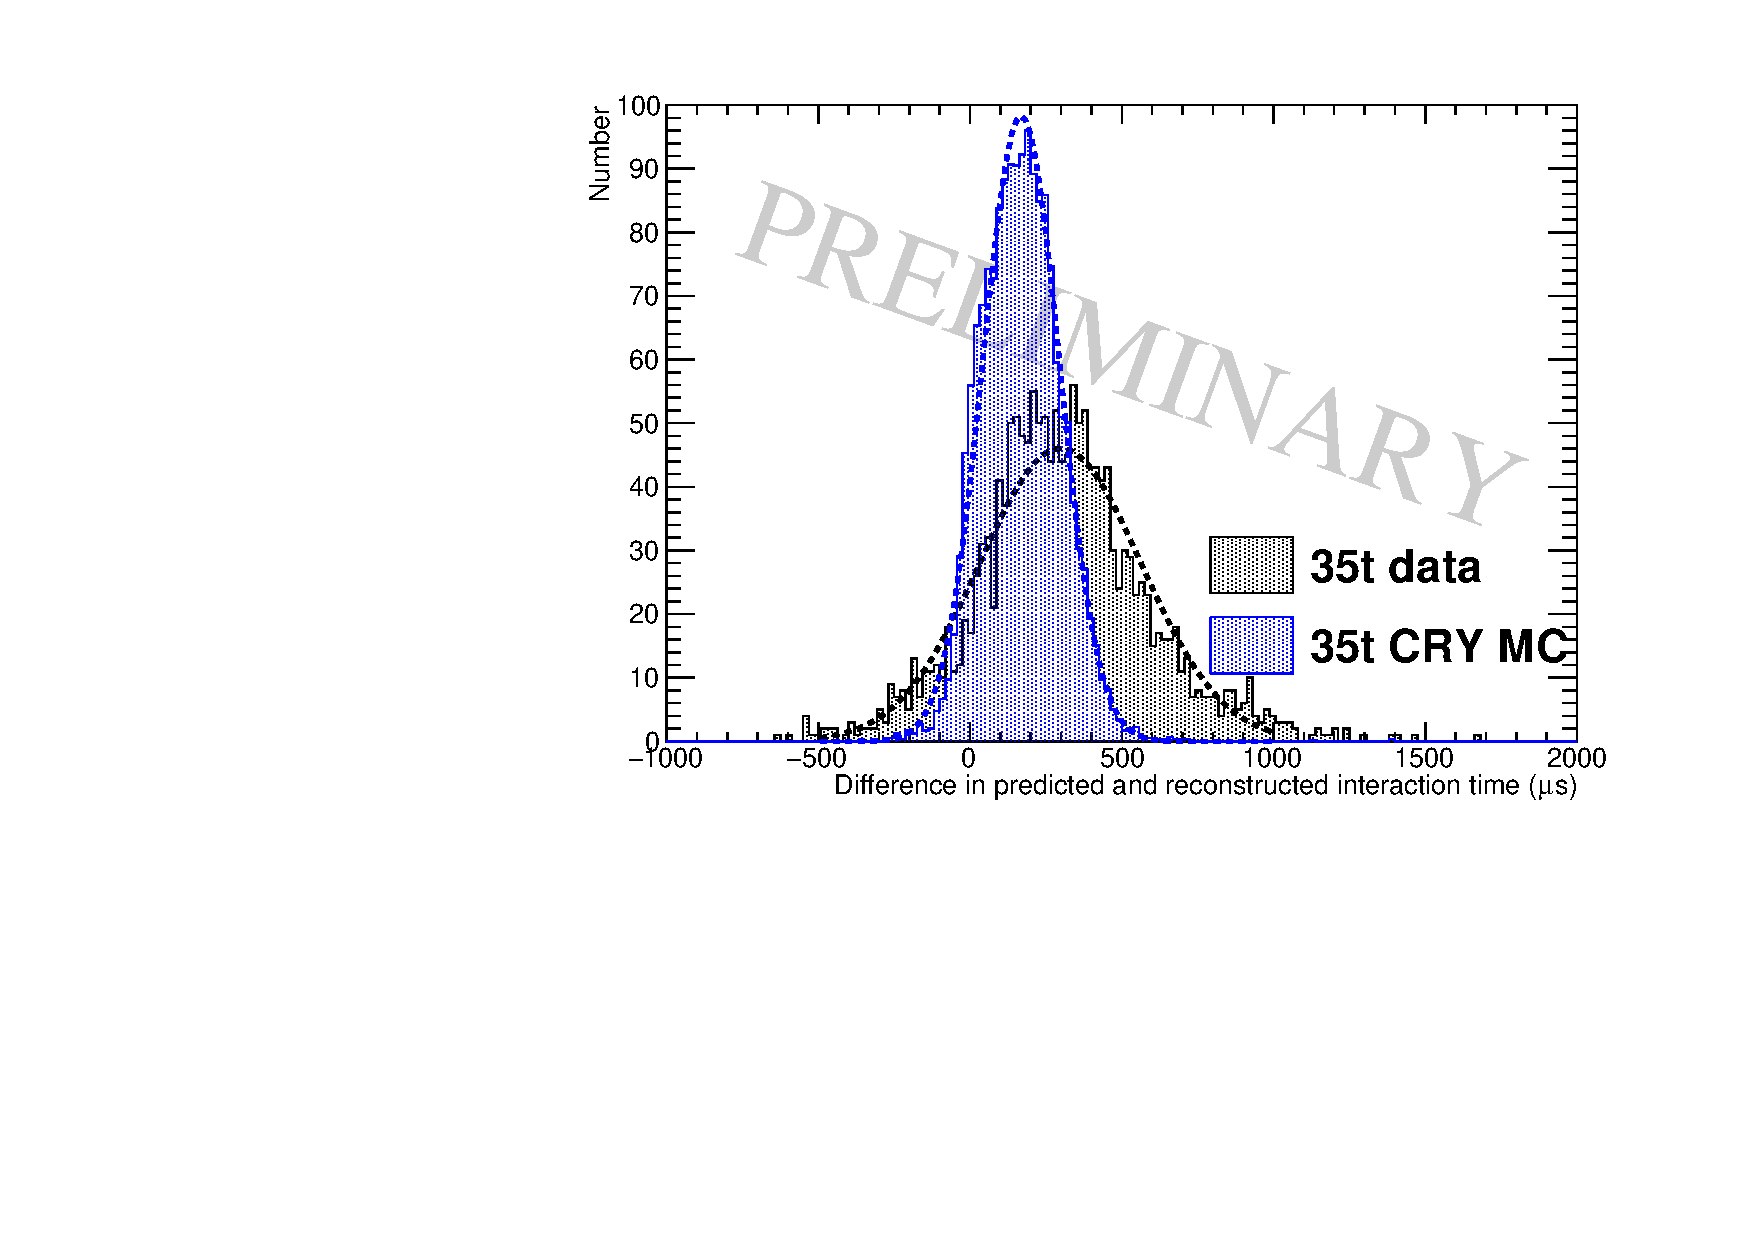
\includegraphics[width=\textwidth]{PredictedTimeFromRMSFits}
    \caption{The accuracy to which interaction times are determined using the hit $RMS$ metric.}
    \label{fig:DiffMCDataResRMS}
  \end{subfigure}
  \hspace{0.08\textwidth}
  \begin{subfigure}{0.45\textwidth}
    \centering
    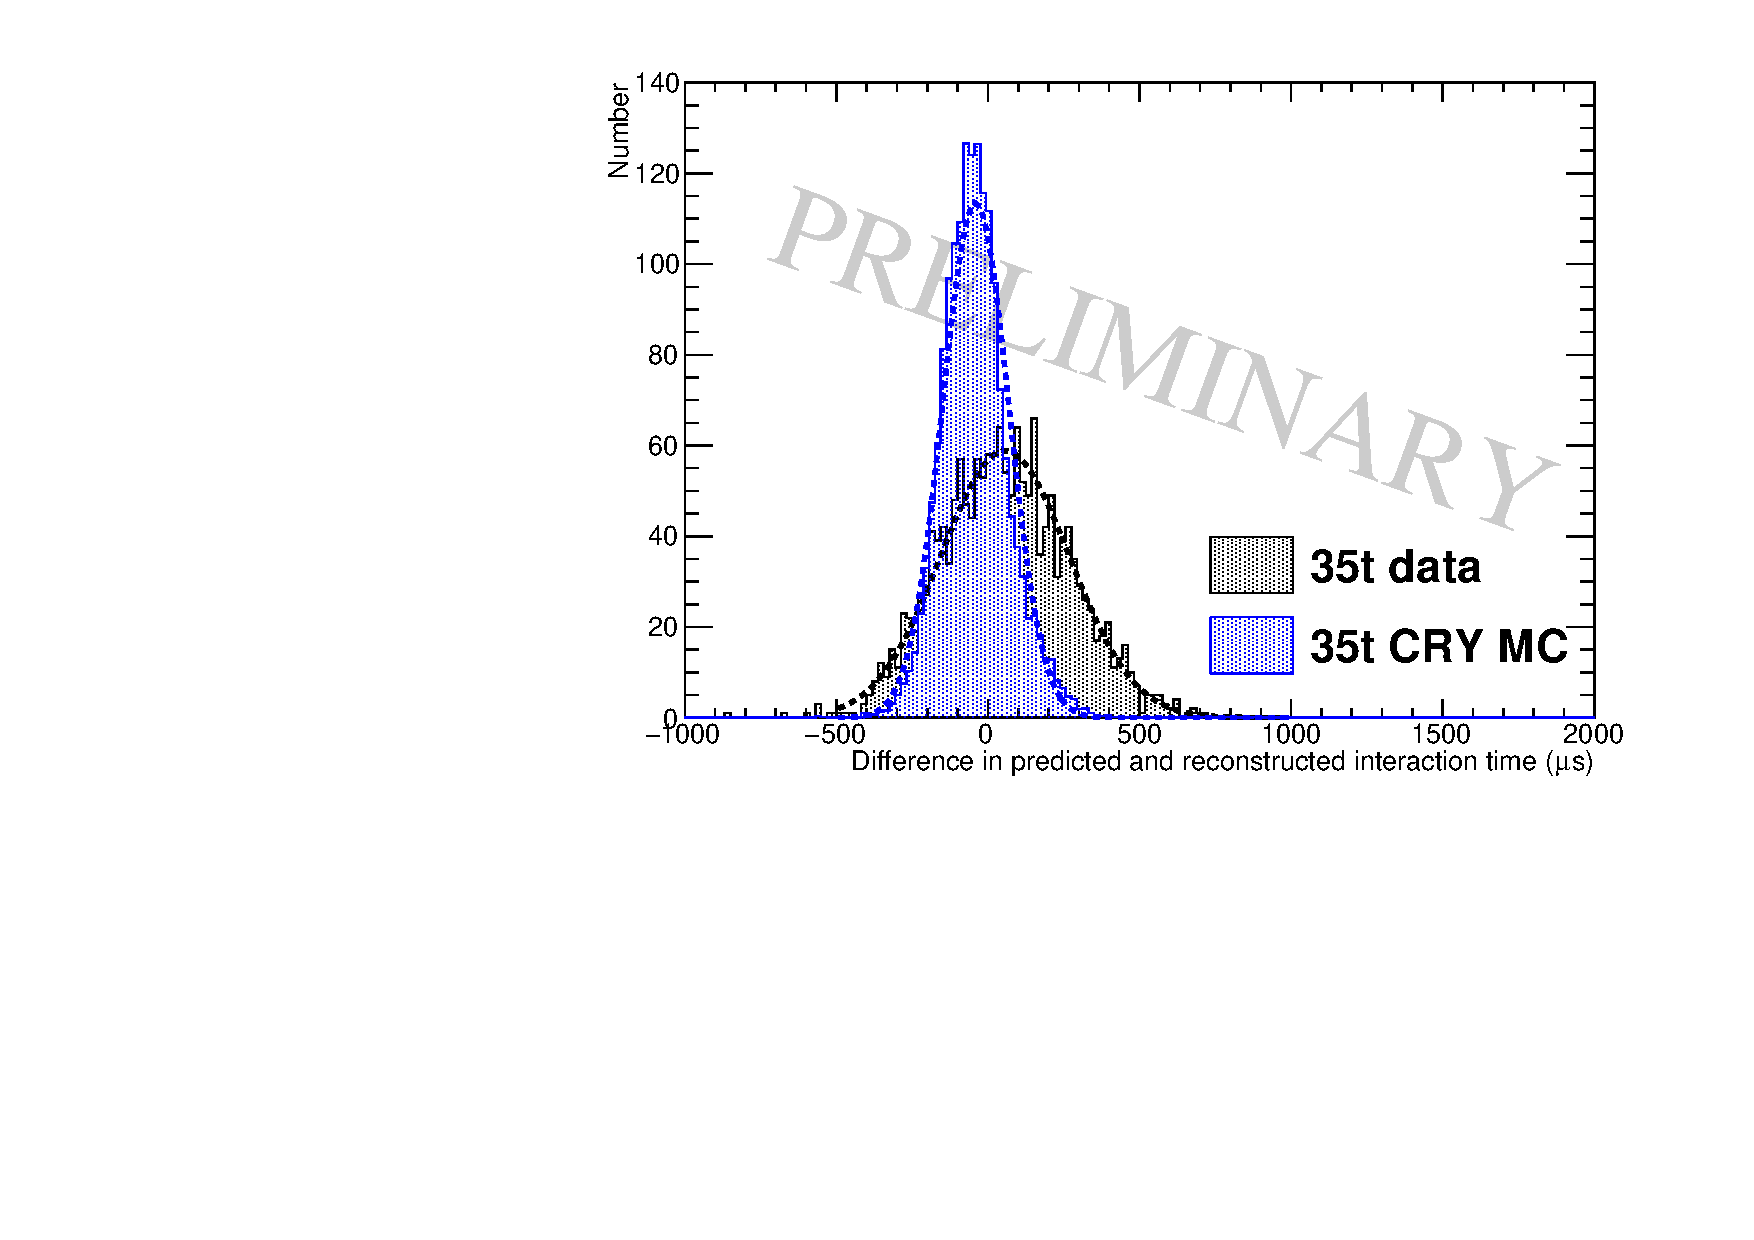
\includegraphics[width=\textwidth]{PredictedTimeFromRMS_IntFits}
    \caption{The accuracy to which interaction times are determined using the hit $RMS/Charge$ metric.}
    \label{fig:DiffMCDataResRMSQ}
  \end{subfigure}
  \caption[A comparison of the accuracy of the interaction time prediction metrics for the low noise Monte Carlo and data 35 ton samples]
          {A comparison of the accuracy of the interaction time prediction metrics for the low noise Monte Carlo and data 35 ton samples for both the $RMS$ and $RMS/Charge$ prediction metrics. The distributions from the 35 ton data are shown in black, whilst the distributions from the low noise simulation are shown in blue.}
          \label{fig:DiffMCDataRes}
\end{figure}

The calculation of interaction times is clearly much better in the low noise Monte Carlo than in the 35 ton dataset, however the distributions are still not centred around 0 implying that there is a systematic error in the method which has not been removed when considering a low noise environment. Looking at Figure~\ref{fig:DiffMCHitFit} the impact of delta rays can still be seen where the $RMS$ plot still has quite a significant tail above the most probable value. This will cause the predicted interaction times to be skewed towards larger times as the hits containing delta rays will be wider and so appear to come at later times than they actually do. Hits containing unseparated delta rays are difficult to remove without looking for slight dips in the raw signals caused by the delta ray beginning to separate from the main track. This would be almost impossible in the 35 ton dataset given the oscillatory nature of the noise. Delta rays can also offer an explanation for the $RMS/Charge$ plot underestimating interaction time as hits containing delta rays would deposit more charge and this increased charge would likely be larger than the increased width, causing the $RMS/Charge$ to decrease. This is seen in Figure~\ref{fig:DiffMCHitFit} where both the data and Monte Carlo samples have consistent tails at small values of $RMS/Charge$, this decrease would then lead to an underestimate of the interaction time. The increased noise level in the 35 ton dataset still causes an overestimation of interaction time, but the most probable difference in predicted and reconstructed interaction times is lower using the $RMS/Charge$ metric than the $RMS$ metric in data suggesting this effect is still present. \\

The widths of the distributions shows that whilst tracks can be disentangled over an entire drift window it is potentially difficult to do so over periods of around 100 $\mu$s, this width is likely due to interpreting distributions which are not Gaussian as Gaussian. This may mean that more sophisticated fits to the distributions used to make the prediction metrics are required which take into account the tails of the distributions as opposed to focusing only on the peaks. The non-Gaussian nature of the distributions will also affect the assumption that over a large number of hits the Gaussian nature of the hit distribution would tend to dominate as if this is not true then one would expect to measure a wide distribution of interaction hit times. It appears that this is the case and that the tails seen in Figure~\ref{fig:DiffMCHitFit} are causing the predicted hit time distribution to be too broad. This feature could potentially be suppressed by performing a fit to the difference in predicted and reconstructed hit times for a track as opposed to taking an average. 

%********************************** % Fifth.Third Section  *************************************
\subsection{Discerning the impact of noise and electron lifetime in Monte Carlo} \label{sec:DiffMCStudies}
Many of the difficulties with the reconstruction and analysis of the 35 ton data have been explained by stating that the noise level made studies difficult, it is important to verify these claims with a study showing the effect of increased noise on the accuracy of the interaction time predicted metrics. This study has been done using the same muons used in the previous Monte Carlo sample with only the noise level of the detector being increased and the inclusion of the noise mitigation algorithms to attempt to reduce the effects of noise as is done in the data sample. The results of this study are shown in Figure~\ref{fig:DiffNoiseComp}, where the metric distributions for tracks with a counter difference of 4 are shown at 20 cm in Figures~\ref{fig:DiffNoiseComp1} and~\ref{fig:DiffNoiseComp2}, the most probable values of hit $RMS$ for tracks due to a counter difference of 4 at all drift distances and the most probable values of hit $RMS$ at $x =$ 0 cm for all counter differences are shown in Figures~\ref{fig:DiffNoiseComp3} and~\ref{fig:DiffNoiseComp4} respectively and the accuracy of the metrics are shown in Figures~\ref{fig:DiffNoiseComp5} and~\ref{fig:DiffNoiseComp6}. \\

\begin{figure}[h!]
  \centering
  \begin{subfigure}{0.45\textwidth}
    \centering
    %\includegraphics[width=\textwidth]{}
    \caption{The distribution of hit $RMS$ values at $x =$ 20 cm.}
    \label{fig:DiffNoiseComp1}
  \end{subfigure}
  \hspace{0.08\textwidth}
  \begin{subfigure}{0.45\textwidth}
    \centering
    %\includegraphics[width=\textwidth]{}
    \caption{The distribution of hit $RMS/Charge$ values at $x =$ 20 cm.}
    \label{fig:DiffNoiseComp2}
  \end{subfigure}
  \begin{subfigure}{0.45\textwidth}
    \centering
    %\includegraphics[width=\textwidth]{}
    \caption{The most probable hit $RMS$ values for tracks with a counter difference of 4.}
    \label{fig:DiffNoiseComp3}
  \end{subfigure}
  \hspace{0.08\textwidth}
  \begin{subfigure}{0.45\textwidth}
    \centering
    %\includegraphics[width=\textwidth]{}
    \caption{The most probable hit $RMS$ values at $x = $ 0 for a range of track angles.}
    \label{fig:DiffNoiseComp4}
  \end{subfigure}
  \begin{subfigure}{0.45\textwidth}
    \centering
    %\includegraphics[width=\textwidth]{}
    \caption{The accuracy to which interaction times are determined using the hit $RMS$ metric.}
    \label{fig:DiffNoiseComp5}
  \end{subfigure}
  \hspace{0.08\textwidth}
  \begin{subfigure}{0.45\textwidth}
    \centering
    %\includegraphics[width=\textwidth]{}
    \caption{The accuracy to which interaction times are determined using the hit $RMS/Charge$ metric.}
    \label{fig:DiffNoiseComp6}
  \end{subfigure}
  \caption[The effect that an increased noise level has on the accuracy of interaction time determination]
          {A study into how increased noise affects the accuracy to which interactions can be determined in the 35 ton.}
          \label{fig:DiffNoiseComp}
\end{figure}

!!!!!! EXPLANATIONS OF WHAT IT LOOKS LIKE !!!!!!! \\

Another important constraint on the effectiveness of interaction time determination is the electron lifetime of the liquid Argon. As the electron lifetime increase fewer electrons will recombine as they drift towards to the APAs meaning that the amount of charge collected will be less affected by the drift distance, potentially greatly affecting the accuracy of the hit $RMS/Charge$ metric. The results of a study to observe the effect of increased electron lifetime are shown in Figure~\ref{fig:DiffLifetimeComp}. \\

\begin{figure}[h!]
  \centering  \begin{subfigure}{0.45\textwidth}
    \centering
    %\includegraphics[width=\textwidth]{}
    \caption{The distribution of hit $RMS$ values at $x =$ 20 cm.}
    \label{fig:DiffLifetimeComp1}
  \end{subfigure}
  \hspace{0.08\textwidth}
  \begin{subfigure}{0.45\textwidth}
    \centering
    %\includegraphics[width=\textwidth]{}
    \caption{The distribution of hit $RMS/Charge$ values at $x =$ 20 cm.}
    \label{fig:DiffLifetimeComp2}
  \end{subfigure}
  \begin{subfigure}{0.45\textwidth}
    \centering
    %\includegraphics[width=\textwidth]{}
    \caption{The most probable hit $RMS$ values for tracks with a counter difference of 4.}
    \label{fig:DiffLifetimeComp3}
  \end{subfigure}
  \hspace{0.08\textwidth}
  \begin{subfigure}{0.45\textwidth}
    \centering
    %\includegraphics[width=\textwidth]{}
    \caption{The most probable hit $RMS$ values at $x = $ 0 for a range of track angles.}
    \label{fig:DiffLifetimeComp4}
  \end{subfigure}
  \begin{subfigure}{0.45\textwidth}
    \centering
    %\includegraphics[width=\textwidth]{}
    \caption{The accuracy to which interaction times are determined using the hit $RMS$ metric.}
    \label{fig:DiffLifetimeComp5}
  \end{subfigure}
  \hspace{0.08\textwidth}
  \begin{subfigure}{0.45\textwidth}
    \centering
    %\includegraphics[width=\textwidth]{}
    \caption{The accuracy to which interaction times are determined using the hit $RMS/Charge$ metric.}
    \label{fig:DiffLifetimeComp6}
  \end{subfigure}
  \caption[The effect that an increased electron lifetime has on the accuracy of interaction time determination]
          {A study into how increased noise affects the accuracy to which interactions can be determined in the 35 ton.}
          \label{fig:DiffLifetimeComp}
\end{figure}

!!!!!! EXPLANATIONS OF WHAT IT LOOKS LIKE !!!!!!! \\

The electric field in all of these studies has been 250 V cm$^{-1}$, however diffusion is known to be affected by the applied electric field. Many LArTPC detectors, including DUNE, are being designed to have an electric field of 500 V cm$^{-1}$ and so it is important to observe the effect which a higher electric field has on the accuracy of the method. An intermediate field of 375 V cm$^{-1}$ is considered as this was the next planned electric field for the 35 ton data taking before the filtration pump breakage stopped data taking. The results of a study to observe the effect of increased electric field are shown in Figure~\ref{fig:DiffEFieldComp}. \\

\begin{figure}[h!]
  \centering  \begin{subfigure}{0.45\textwidth}
    \centering
    %\includegraphics[width=\textwidth]{}
    \caption{The distribution of hit $RMS$ values at $x =$ 20 cm.}
    \label{fig:DiffEFieldComp1}
  \end{subfigure}
  \hspace{0.08\textwidth}
  \begin{subfigure}{0.45\textwidth}
    \centering
    %\includegraphics[width=\textwidth]{}
    \caption{The distribution of hit $RMS/Charge$ values at $x =$ 20 cm.}
    \label{fig:DiffEFieldComp2}
  \end{subfigure}
  \begin{subfigure}{0.45\textwidth}
    \centering
    %\includegraphics[width=\textwidth]{}
    \caption{The most probable hit $RMS$ values for tracks with a counter difference of 4.}
    \label{fig:DiffEFieldComp3}
  \end{subfigure}
  \hspace{0.08\textwidth}
  \begin{subfigure}{0.45\textwidth}
    \centering
    %\includegraphics[width=\textwidth]{}
    \caption{The most probable hit $RMS$ values at $x = $ 0 for a range of track angles.}
    \label{fig:DiffEFieldComp4}
  \end{subfigure}
  \begin{subfigure}{0.45\textwidth}
    \centering
    %\includegraphics[width=\textwidth]{}
    \caption{The accuracy to which interaction times are determined using the hit $RMS$ metric.}
    \label{fig:DiffEFieldComp5}
  \end{subfigure}
  \hspace{0.08\textwidth}
  \begin{subfigure}{0.45\textwidth}
    \centering
    %\includegraphics[width=\textwidth]{}
    \caption{The accuracy to which interaction times are determined using the hit $RMS/Charge$ metric.}
    \label{fig:DiffEFieldComp6}
  \end{subfigure}
  \caption[The effect that an increased electric field has on the accuracy of interaction time determination]
          {A study into how increased noise affects the accuracy to which interactions can be determined in the 35 ton.}
          \label{fig:DiffEFieldComp}
\end{figure}

!!!!!! EXPLANATIONS OF WHAT IT LOOKS LIKE !!!!!!!

%********************************** % Fifth.Fourth Section  *************************************
\subsection{The limitations of and future improvements to the method of interaction time determination using diffusion} \label{sec:DiffLimitations}
sdfsdsdas
